% This template was initially provided by Dulip Withanage.
% Modifications for the database systems research group
% were made by Conny Junghans,  Jannik Strötgen and Michael Gertz

\documentclass[
     12pt,         % font size
     a4paper,      % paper format
     BCOR10mm,     % binding correction
     DIV14,        % stripe size for margin calculation
%     liststotoc,   % table listing in toc
%     bibtotoc,     % bibliography in toc
%     idxtotoc,     % index in toc
%     parskip       % paragraph skip instad of paragraph indent
     ]{scrreprt}

%%%%%%%%%%%%%%%%%%%%%%%%%%%%%%%%%%%%%%%%%%%%%%%%%%%%%%%%%%%%

% PACKAGES:

% Use German :
\usepackage[english]{babel}
% Input and font encoding
\usepackage[latin1]{inputenc}
\usepackage[T1]{fontenc}
% Index-generation
\usepackage{makeidx}
% Einbinden von URLs:
\usepackage{url}
% Special \LaTex symbols (e.g. \BibTeX):
%\usepackage{doc}
% Include Graphic-files:
\usepackage{graphicx}
% Include doc++ generated tex-files:
%\usepackage{docxx}
% Include PDF links
%\usepackage[pdftex, bookmarks=true]{hyperref}
\usepackage[acronym, nonumberlist]{glossaries}

\usepackage{csquotes}




% Fuer anderthalbzeiligen Textsatz
\usepackage{setspace}

% hyperrefs in the documents
\usepackage[bookmarks=true,colorlinks,pdfpagelabels,pdfstartview = FitH,bookmarksopen = true,bookmarksnumbered = true,linkcolor = black,plainpages = false,hypertexnames = false,citecolor = black,urlcolor=black]{hyperref} 
%\usepackage{hyperref}

%%%%%%%%%%%%%%%%%%%%%%%%%%%%%%%%%%%%%%%%%%%%%%%%%%%%%%%%%%%%

% OTHER SETTINGS:

% Pagestyle:
\pagestyle{headings}

% Choose language
\newcommand{\setlang}[1]{\selectlanguage{#1}\nonfrenchspacing}

% Acronym definition
\makeglossaries
\newacronym{qa}{QA}{Question Answering}
\newacronym{ai}{AI}{Artificial Intelligence}
\newacronym{ml}{ML}{Machine Learning}
\newacronym{dl}{DL}{Deep Learning}
\newacronym{convqa}{Conv QA}{Conversational Question Answering}
\newacronym{mit}{MIT}{Massachusetts Institute of Technology}
\newacronym{trec}{TREC}{Text REtrieval Conference}
\newacronym{ir}{IR}{Information Retrieval}
\newacronym{nn}{NN}{Neural Network}
\newacronym{s2s}{seq-2-seq}{Sequence-to-Sequence}
\newacronym{kb}{KB}{Knowledge Base}
\newacronym{mrc}{MRC}{Machine Reading Comprehension}
\newacronym{rag}{RAG}{Retrieval-Augmented Generation}
\newacronym{realm}{REALM}{Retrieval-Augmented Language Model pre-training}
\newacronym{docvqa}{DocVQA}{Document Visual Question Answering}
\newacronym{ocr}{OCR}{Optical Character Recognition}
\newacronym{llm}{LLM}{Large Language Model}
\newacronym{dpr}{DPR}{Dense Passage Retrieval}
\newacronym{bert}{BERT}{Bidirectional Encoder Representations from Transformers}
\newacronym{prlm}{PrLM}{Transformer-based Pre-trained Language Model}

\glsaddall

\begin{document}

% TITLE:
\pagenumbering{roman} 
\begin{titlepage}


\vspace*{1cm}
\begin{center}
\vspace*{3cm}
\textbf{ 
\Large Universität Heidelberg\\
\smallskip
\Large Institut für Informatik\\
\smallskip
\Large Arbeitsgruppe Datenbanksysteme\\
\smallskip
}

\vspace{3cm}

\textbf{\large Master-Arbeit} % Bachelor-Arbeit 

\vspace{0.5\baselineskip}
{\huge
\textbf{Building an adaptable and resource constrained Conversational Information Search System}
}
\end{center}

\vfill 

{\large
\begin{tabular}[l]{ll}
Name: & Stephan Lenert\\
Matrikelnummer: & Matrikelnummer  der Autorin/des Autors\\
Betreuer: & Name der Betreuerin / des Betreuers\\
Datum der Abgabe: & \today
\end{tabular}
}

\end{titlepage}

\onehalfspacing

\thispagestyle{empty}

\vspace*{100pt}
\noindent
Ich versichere, dass ich diese Master-Arbeit selbstständig verfasst und nur die angegebenen
Quellen und Hilfsmittel verwendet habe und die Grundsätze und
Empfehlungen ``Verantwortung in der Wissenschaft'' der Universität Heidelberg beachtet wurden. 

\vspace*{50pt}
\noindent

\underline{\phantom{mmmmmmmmmmmmmmmmmmmm}}

\medskip
\noindent 
Abgabedatum: \today
\newpage

% Add a brief summary of your topic and contributions (Zusammenfassung) in German *and* in English:
\chapter*{Zusammenfassung}
Das Interesse an der Entwicklung von Systemen für die konversationelle Informationssuche hat durch ChatGPT stark zugenommen. Jedoch ist eine alleinige Verwendung von ChatGPT aufgrund von Herausforderungen wie der Aktualisierung und Veränderung von Wissen, Halluzinationen oder der Interpretierbarkeit von KI nicht ausreichend. Die Bewältigung dieser Hürden erfordert die Entwicklung von Retriever-Reader-Systemen. Allerdings ist die Konstruktion solcher Systeme für reale Anwendungsfälle in der aktuellen Forschung noch nicht ausreichend abgedeckt. Diese Arbeit schlägt ein umfassendes Rahmenwerk für Retrieval-Augmented Generation (RAG)-basierte konversationelle Frage-Antwort-Systeme vor, das vier Komponenten umfasst: Extractor, Contextual Query Understanding (CQU), Retriever und Reader. Es werden das Problemfeld, die Herausforderungen und Lösungsansätze für jede Komponente beschrieben, wobei der Fokus darauf liegt, bestehende Retriever- oder Reader-Modelle zu nutzen, anstatt neue Architekturen zu entwickeln. Für die Herausforderungen im Bereich des Retrievers werden Lösungen vorgeschlagen, die auf PROMPTAGATOR für Probleme im Zusammenhang mit dem Datensatz und verschiedenen Methoden wie Mixture-of-Experts für Probleme im Zusammenhang mit dem Evidence Set basieren. Für die Extract-Komponente wird eine pipelinefähige Kombination von Operationen vorgeschlagen. Die Aufgabe des Readers wird in mehrere kleinere Herausforderungen unterteilt, für die Lösungsansätze basierend auf Fine-Tuning oder Nachbearbeitung des Evidence Sets entwickelt werden. Unter Verwendung dieses Frameworks wird ein beispielhafter Frage-Antwort-Chatbot für die Prüfungsordnung der Universität Heidelberg entwickelt. Die Evaluation dieses Chatbots zeigt Engpässe in den Komponenten Retriever und Extractor auf, hebt die Nachteile kleinerer Sprachmodelle wie Llama2-7B-chat im Vergleich zu größeren Modellen wie gpt-3.5-turbo hervor und unterstreicht die Grenzen synthetischer Daten für die automatische Evaluation, die vor allem nur für faktoide Fragen anwendbar sind.
\newpage

\chapter*{Abstract}
The resurgence of interest in conversational information seeking, reignited by the boom of systems like ChatGPT and large language models in general, faces challenges such as knowledge extension, hallucination, and AI interpretability. Overcoming these hurdles necessitates the development of retriever-reader systems, yet constructing such systems from scratch for real-world use cases remains underexplored in current research. This thesis proposes a comprehensive framework for retrieval-augmented generation (RAG)-based conversational question-answering, comprising four components: Extractor, Contextual Query Understanding (CQU), Retriever, and Reader. We delineate the problem field, challenges, and solutions for each component, focusing on leveraging existing Retriever or Reader models rather than reinventing them. We address challenges in the Retriever, proposing solutions based on synthetic data for knowledge source challenges and various methods such as Mixture-of-Experts for evidence set challenges. For the Extract component, we propose a pipeline combination of operations. The Reader's task is broken down into multiple micro challenges and proposes solutions for them based on fine-tuning or post-processing of the evidence set. Applying this framework, we develop an exemplary question-answering chatbot for Heidelberg University's examination regulations. Evaluation uncovers bottlenecks in the Retriever and Extractor components, highlights the drawbacks of smaller language models like Llama2-7B-chat compared to larger models like gpt-3.5-turbo, and emphasizes the limitations of synthetic data for automatic evaluation, primarily applicable to factoid questions. 
\newpage

% MAIN PART:
% Table of contents (Inhaltsverzeichnis)
\tableofcontents
\cleardoublepage
\pagenumbering{arabic} 

% List of acronyms (Abkürzungsverzeichnis):
\chapter*{List of Acronyms}
\printglossary[type=\acronymtype]

% List of figures (Abbildungsverzeichnis):
\listoffigures
% List of tables (Tabellenverzeichnis):
\listoftables

%%%%%%%%%%%%%%%%%%%%%%%%%%%%%%%%%%%%%%%%%%%%%%%%%%%%%%%%%%%%%%%
% Here, the actual content of your thesis begins
% You can either put all the text here or use individual files to store the chapters of your thesis.
% Below are templates for both alternatives.


\chapter{Introduction}
\label{chap:intro}
\section{Motivation}

The journey of exploring natural language querying dates back to as early as 1961, with researchers embarking on projects like Baseball \cite{green_baseball_1961}, a program designed to respond to users' natural language queries within the domain of baseball. In 1999, the \gls{trec} initiated the \gls{trec}-8 Question Answering track, marking \enquote{the first large-scale evaluation of domain-independent question-answering systems} \cite{voorhees_trec-8_1999}. A more renowned \gls{qa} system is IBM's \textit{Watson}, an open-domain \gls{qa} system that famously triumphed on the television game show Jeopardy! in 2011 \cite{ferrucci_introduction_2012}. The advent of conversational assistants such as Alexa, Siri, and Cortana further fueled interest in conversational information seeking. In 2019, the establishment of the \gls{trec} \gls{cast} aimed to nurture \gls{cis} as an active research field and provide large-scale reusable test beds. However, the true surge in user engagement came with the release of ChatGPT by OpenAI in November 2022, which achieved an astounding one million users within five days \cite{demandsage2022chatgpt}.

Since the widespread adoption of ChatGPT, interest in conversational information seeking has surged once again. However, using a generative \gls{llm} only has certain drawbacks, including the following:

\begin{enumerate}
    \item Parameterized Knowledge: Expansion or updating of knowledge is challenging.
    \item Explainability: Understanding the rationale behind predictions is difficult.
    \item Hallucination: The model may invent seemingly factual information not present in the underlying knowledge source.
\end{enumerate}

These limitations render the sole use of generative models inadequate for practical conversational information-seeking use cases. Consequently, researchers have explored various approaches to address these issues and develop conversational information-seeking systems that mimic human-like conversations \cite{ferrucci_introduction_2012,guu_realm_2020,lewis_retrieval-augmented_2021,nakano_webgpt_2022}. Among these approaches, \gls{rag} \cite{lewis_retrieval-augmented_2021} has emerged as a leading solution, evident in trending frameworks like Langchain \cite{noauthor_question_nodate} and even ChatGPT itself \cite{noauthor_chatgpt_2023}.

However, despite advancements in research, there is a notable absence of papers detailing the adoption of these techniques in real-world use cases. To our knowledge, only two such papers exist \cite{feng_dialdoc_2021,gholami_zero-shot_2021}, which do not comprehensively address the entire problem domain associated with this task, such as the extraction step, and fail to leverage modern possibilities with \gls{llm}s.

\section{Objectives and Contributions}

This thesis aims to bridge this gap by addressing the question of how to build a faithful conversational question-answering system for real-world use cases, a topic that has not been adequately explored in scientific literature to date. This thesis resolves this issue by firstly laying out the fundamental concepts and techniques necessary, secondly developing a holistic framework for constructing such a system based on \gls{rag}, and thirdly implementing a \gls{poc} based on the examination regulations of Heidelberg University. Finally, we evaluate the \gls{poc} using synthetic data and human evaluation. The core contributions of this thesis are as follows:

\begin{itemize}
    \item Providing a holistic overview of the challenges in conversational question-answering systems tailored to a specific document collection and developing a comprehensive framework for constructing such systems based on the four components: Extract, CQU, Retriever and Reader.
    \item Breaking down the extraction of passages from a document collection into pipeline operations.
    \item Identifying challenges faced by the Retriever component towards both the knowledge base and the evidence set and how to resolve them using synthetic-data-based fine-tuning and Mixture-of-Experts.
    \item Decomposing the task of the Reader component into micro-challenges and proposing solutions for them.
    \item Offering multiple approaches for evaluating conversational question-answering systems, with the major insight, that the component-wise evaluation for non-factoid questions needs new approaches and currently at least in the case of this thesis, the human end-to-end evaluation was the most robust approach.
    \item Highlighting the limitations of synthetic data for system evaluation, as those can only be used for factoid question generation due to the used pattern of question-context-answer tuples.
    \item Providing insights into the current bottlenecks of use-case-specific \gls{convqa} systems. Mainly the retriever component and the associated extraction of passages are drawbacks. In the end-to-end evaluation, 46.5\% of errors were attributed to the retriever component and 18.5\% to the extraction component directly.
\end{itemize}

Those cover the main contributions and insights of this thesis, for detailed insights, please refer to the respective chapters. 

\section{Thesis Structure}

The construction of a conversational question-answering system is approached in two stages within this thesis. Firstly, we focus on question-answering based on a single natural language query, followed by the addition of the conversational component. Thus, Chapter \ref{chap:grundlagen} provides a comprehensive overview. Section \ref{sec:qa} presents various approaches and concepts in the field of question-answering, while Section \ref{sec:cqa} extends this perspective to include conversational elements. Narrowing down the range of potential solutions, Chapter \ref{chap:main} introduces the \gls{conrag} framework, which lays out the spectrum of challenges, from handling document collections to enabling conversational question-answering. It's important to note that we streamline the choice of possible implementations to a system consisting of four distinct components: Extract, CQU, Retriever and Reader. The validation of this newly established system approach is conducted in a \gls{poc} manner in Chapter \ref{chap:eval}. Here, we implement and evaluate an exemplary system using the collection of examination regulations from Heidelberg University. This chapter also includes insightful reflections on the evaluation of conversational question-answering systems. This concludes the content outline of this thesis.


%%%%%%%%%%%%%%%%%%%%%%%%%%%%%%%%%%%%%%%%%%%%%%%%%%%%%%%%%%%%
\newpage
%%%%%%%%%%%%%%%%%%%%%%%%%%%%%%%%%%%%%%%%%%%%%%%%%%%%%%%%%%%%

\chapter{Background and Related Work}
\label{chap:grundlagen}

This chapter provides essential background information and reviews relevant prior research. It commences with an introduction to the sub-task of Question Answering (\gls{qa}), as presented in Section \ref*{sec:qa}. As previously mentioned in the Introduction (Chapter \ref{chap:intro}), this chapter maintains a clear distinction between \gls{qa} and \gls{convqa}. Consequently, Section \ref{sec:cqa} extends upon the foundational knowledge of \gls*{qa} and introduces the requisite concepts for the transformation of a QA-System into a \gls{convqa}-System. Section \ref{sec:related_work} will delve into the related work, providing a comprehensive overview of the current state-of-the-art in the field of \gls{qa} and \gls{convqa} over textual knowledge sources.

\section{Question Answering}
\label{sec:qa}

The evolution of \gls{qa} as a research field provides a solid foundation for understanding current research initiatives and methodologies. Among the early contributions is BASEBALL, an automated \gls{qa} system developed by researchers at \gls{mit} in 1961. This QA system demonstrated its capability to answer questions related to baseball using natural English language \cite{green_baseball_1961}.


In 1999, \gls{trec} (Text Retrieval Conference) initiated the \gls{trec}-8 Question Answering track, which marked "the first large-scale evaluation of domain-independent question-answering systems" \cite{voorhees_trec-8_1999}. A more well-known QA system is \textit{Watson} by IBM, an open-domain \gls{qa} system that won a the TV show Jeopardy! in 2011 \cite{ferrucci_introduction_2012}. It is evident that an evolutionary process has occurred between the early research in 1961 and today's systems like \textit{ChatGPT} by OpenAI. To understand the dimensions in which these systems differ, their components, and how to distinguish them will be introduced in Section \ref{subsec:qa_basics}, while subsequent sections will delve deeper into specific components.

In 1999, the \gls{trec} initiated the \gls{trec}-8 Question Answering track, marking \enquote{the first large-scale evaluation of domain-independent question-answering systems} \cite{voorhees_trec-8_1999}. A more renowned QA system is IBM's \textit{Watson}, an open-domain \gls{qa} system that famously triumphed on the television game show Jeopardy! in 2011 \cite{ferrucci_introduction_2012}. It is evident that an evolutionary process has transpired between the early research in 1961 and contemporary systems such as OpenAI's \textit{ChatGPT}. In section \ref{subsec:qa_basics} we will lay the groundwork by introducing the fundamental aspects of \gls{qa}-Systems and the techniques used to differentiate and categorize them. Following that, subsequent sections will delve deeper into the examination of specific system components.


\subsection{Basics}
\label{subsec:qa_basics}

Jurafsky and Martin define a \gls{qa}-System as a system \enquote{designed to satisfy human information needs} \cite{jurafsky_speech_2023}. Hence, it primarily functions as an Information Retrieval System, with its primary objective being to provide users with the desired and accurate information in response to natural language requests.

The research community has yet to establish a universally accepted classification framework for Question Answering (QA) systems. For instance, Hao et al. and Farea et al. \cite{hao_recent_2022, farea_evaluation_2022} take a comprehensive approach to classify QA systems but differ in certain aspects, such as their treatment of question types and knowledge sources. On the other hand, other researchers \cite{zhu_retrieving_2021, jurafsky_speech_2023, etezadi_state_2023, zhang_survey_2023} employ a similar classification methodology but often focus solely on retrieval-based approaches, thereby lacking a holistic perspective.

The classification proposed by Farea et al. \cite{farea_evaluation_2022} goes a step further by distinguishing between the \textbf{QA-Framework} and \textbf{QA-Paradigms}, enhancing its versatility for comparing classical and modern QA systems. An adaptation of this classification will be utilized in this thesis. The originally proposed QA algorithms have been extended to include the Retrieval-based approach, and the Question Types have been revised based on the typology introduced by Mishra et al. in their 2016 survey \cite{mishra_survey_2016}, which was further elaborated upon by Etezadi et al. \cite{etezadi_state_2023}. Also the Answer Types where adjusted to align with the classifications used in \cite{mcdonald_detect_2022,dasigi_dataset_2021}. In this context, a crucial distinction is made between a \textbf{QA} and \textbf{ConvQA} system, guided by the criteria outlined in \cite{zamani_conversational_2023}: a QA system exclusively handles standalone questions, while any inquiry exceeding a single question and involving conversational context falls within the domain of a \textbf{ConvQA} system.

The \textbf{\gls{qa}-Framework} encompasses external factors such as Question and Answer Types, while also considering system-related factors like the \gls{qa} Algorithm and Knowledge Source \cite{farea_evaluation_2022, hao_recent_2022}. Conversely, the \textbf{\gls{qa}-Paradigm} defines the fundamental underlying concept of a system and can be seen as a subset of possible combinations within the \textbf{\gls{qa} Framework}. Currently, three dominant paradigms prevail:

\begin{enumerate}
    \item \textbf{Information Retrieval (IR)-Based QA}: This paradigm involves searching through extensive multi-modal data based on a user's question and using the retrieved passages to generate an answer.
    
    \item \textbf{Knowledge Base (KB) QA}: In this approach, a semantic representation of the question is constructed, and a knowledge base is queried using this representation. The returned results are then used to generate an answer.
    
    \item \textbf{Generative Question Answering}: Here, knowledge is fully implicit, and a neural network (NN) generates answers based on its trained parameters.

\end{enumerate}

For visual clarity, a diagram illustrating the adjusted \gls{qa} Framework Classification by Farea et al. is provided in Figure \ref{fig:qa_classification}.

\begin{figure}
    \centering
    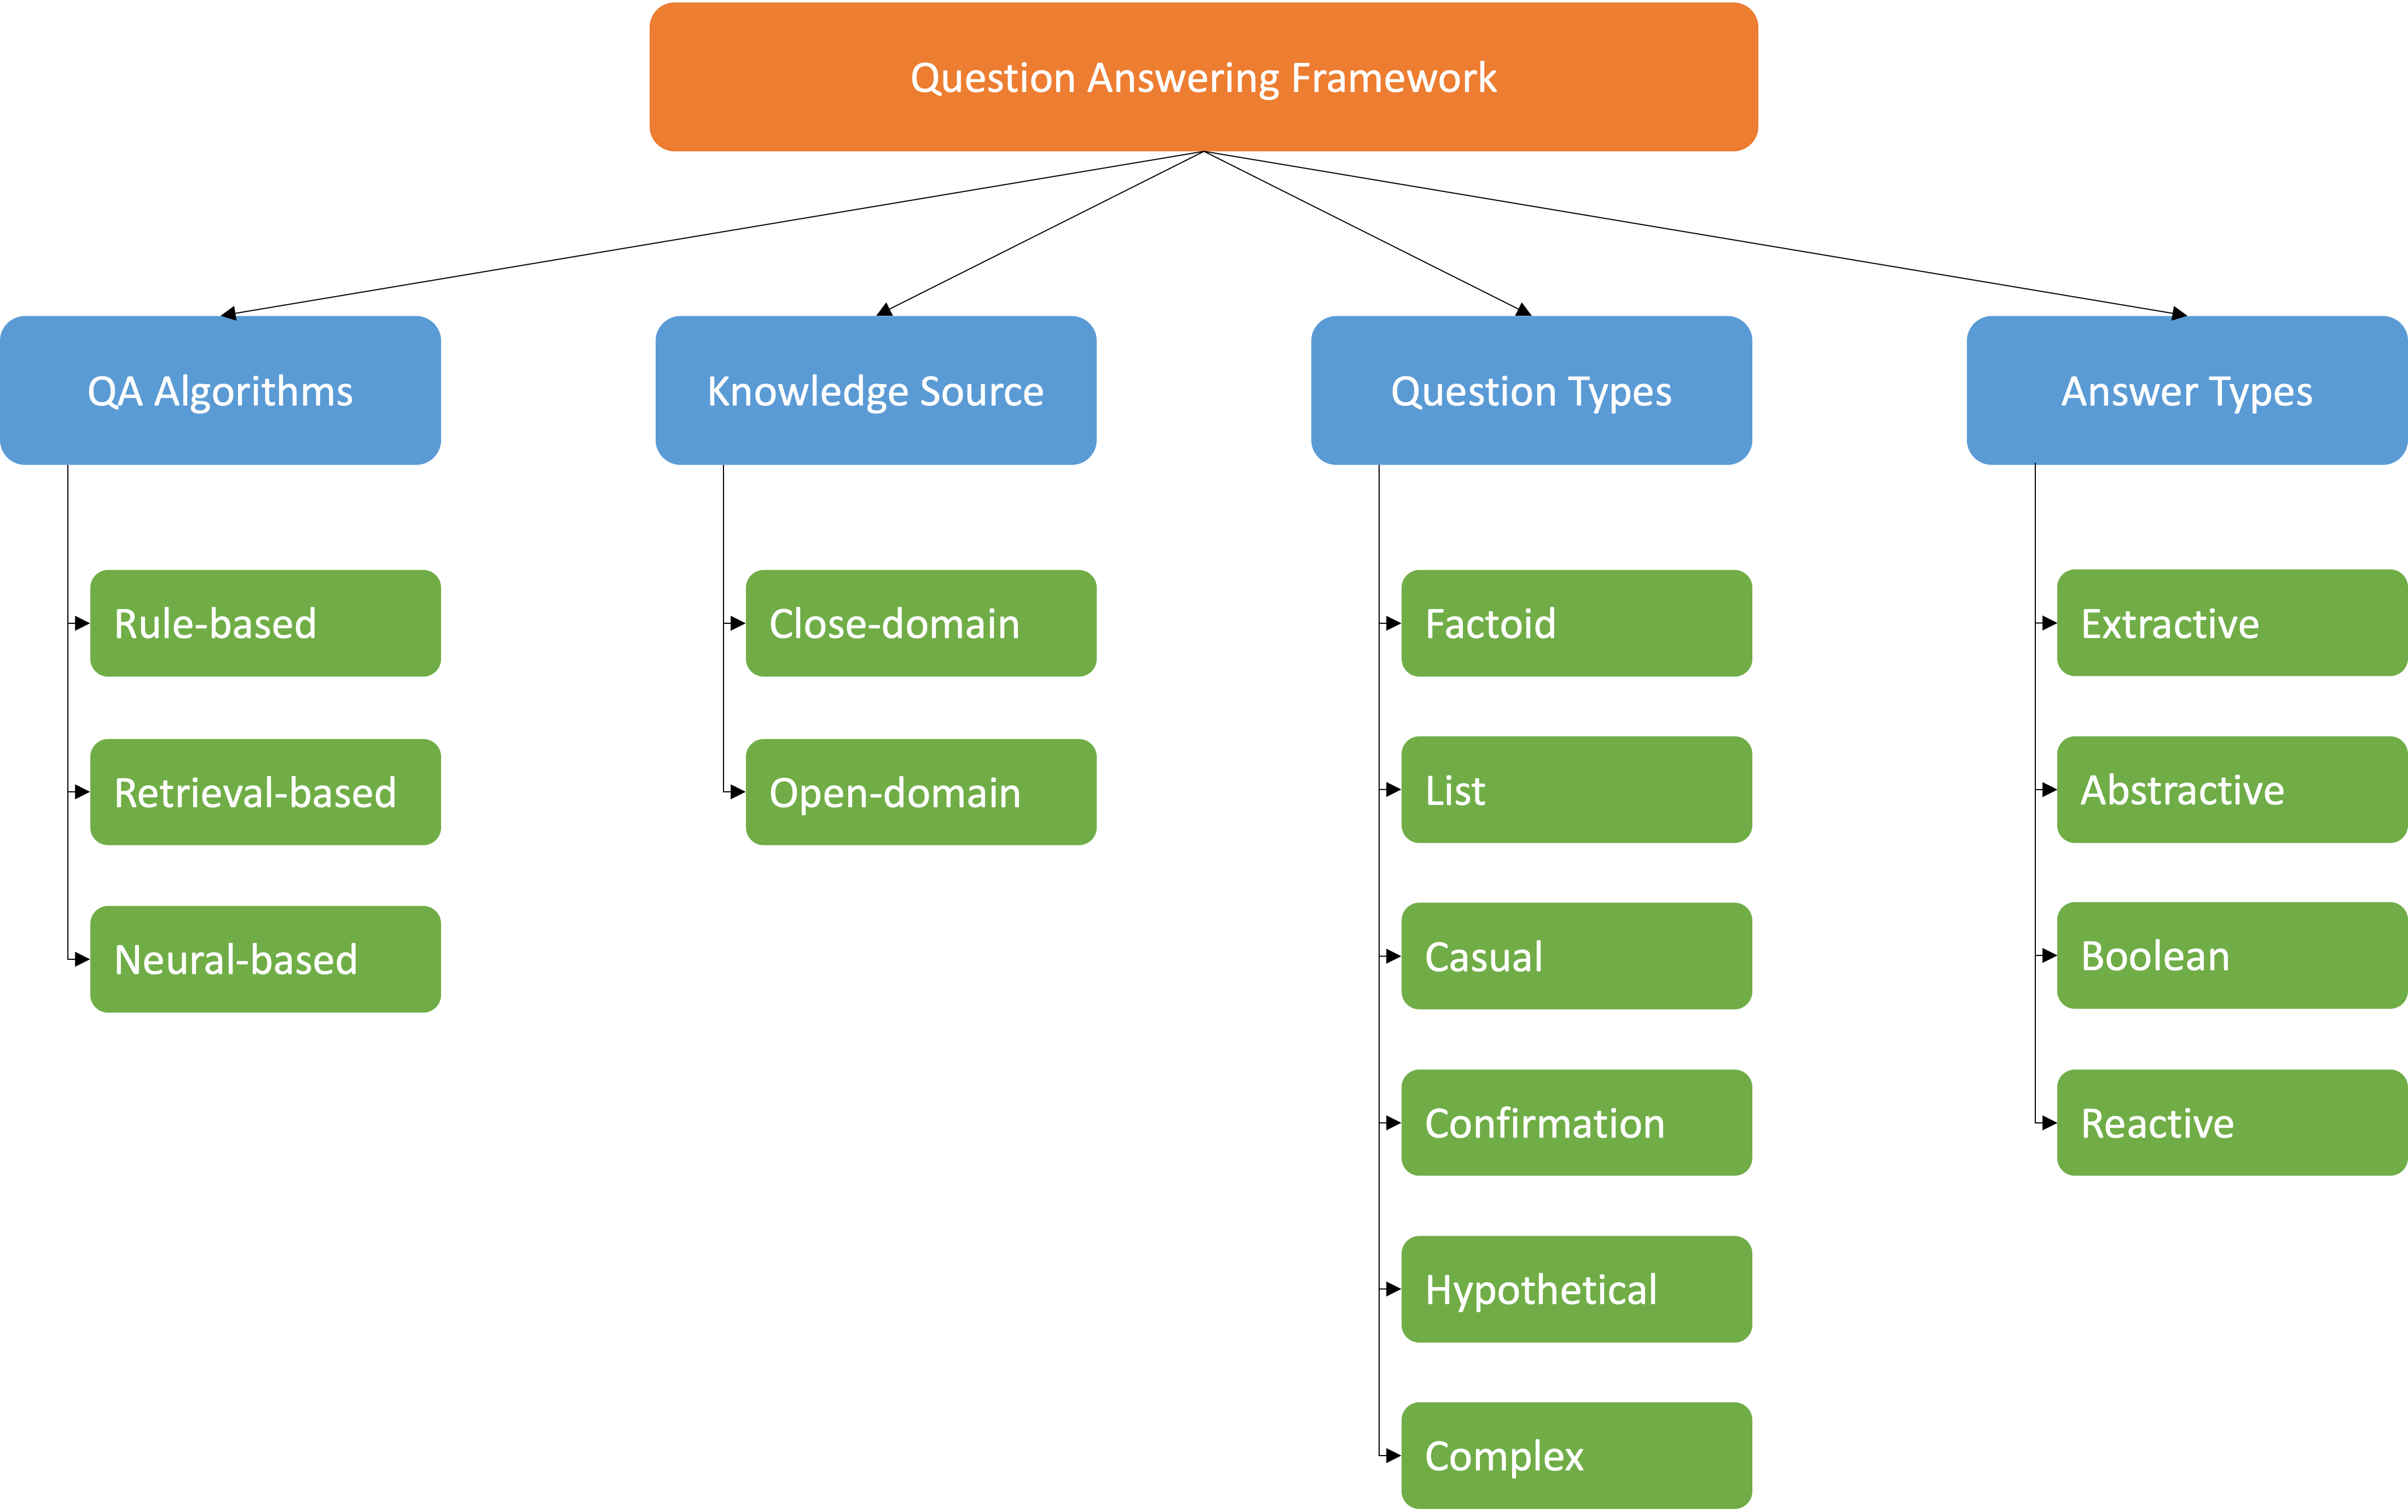
\includegraphics[width=\textwidth]{Grafiken/QA_Framework.png}
    \caption{Adjusted \gls{qa} Framework Classification by Farea et al. \cite{farea_evaluation_2022}}
    \label{fig:qa_classification}
\end{figure}


Figure \ref{fig:qa_classification} illustrates the aforementioned classification. The primary distinguishing factor is the employed \textbf{\gls{qa} Algorithm}. Rule-based approaches involve the manual crafting of feature extractions from user questions, which are then compared to the knowledge base. Rule-based approaches are typically employed in closed-domain \gls{qa} systems exclusively \cite{etezadi_state_2023}.

Retrieval-based approaches are the classic Information Retrieval (IR)-based \gls{qa} systems, comprising two key components: an intent classifier and a retriever. The intent classifier's objective is to discern the question's intent and identify important entities. Subsequently, the retriever searches the knowledge source and identifies the most relevant passages \cite{farea_evaluation_2022, zhu_retrieving_2021}.

The Neural-based approach, often referred to as the generative approach, utilizes a Sequence-to-Sequence (S2S) model to generate accurate answers to given questions. In this paradigm, the information is stored directly in the neural network's parameters, otherwise the neural network is part of a Retrieval-based approach. Most datasets in these contexts consist of triples of question, context, and answer pairs \cite{jurafsky_speech_2023}. Notably, widely used datasets such as SQuAD and QASPER originally emerged from the field of machine reading comprehension, representing a foundational step in the evolution of \gls{qa} systems \cite{rajpurkar_squad_2016, dasigi_dataset_2021, zhu_retrieving_2021}.

In addition to the \textbf{\gls{qa} Algorithms}, the \textbf{Knowledge Source} plays a pivotal role in distinguishing various aspects of Question Answering (QA) systems. The nature of the knowledge source can range from structured to unstructured or semi-structured, and it may encompass diverse data modalities, including text, audio, and video. A common point of comparison in the QA landscape is between closed and open-domain systems.

In the broad sense, a \textbf{closed-domain} QA system operates within the confines of a specific knowledge domain, which means it has limited access to information. In contrast, \textbf{open-domain} QA systems grapple with an extensive array of knowledge sources, necessitating a more versatile approach \cite{farea_evaluation_2022}.

Furthermore, a closed-domain setup often entails limitations on the types of questions it can handle, primarily focusing on factoid questions or predefined templates. Additionally, it frequently relies on structured knowledge bases like graphs or logically organized repositories \cite{hao_recent_2022}.

Conversely, open-domain QA systems are designed to tackle a wide spectrum of user queries, ranging from factoids to more complex inquiries. They typically deal with unstructured knowledge sources, which can be substantial and diverse in content \cite{zhu_retrieving_2021, farea_evaluation_2022, jurafsky_speech_2023}.

An alternative perspective for distinguishing \gls{qa}-Systems lies in the \textbf{Question Types} that users can input into the system. Questions can fall into various categories, such as \textit{factoid, list, casual, confirmation, hypothetical} \cite{mishra_survey_2016}, or \textit{complex} \cite{etezadi_state_2023}.

\begin{itemize}
   \item \textit{Factoid questions}, the most common type, are typically signaled by question words (what, when, which, who, how) and yield a concise factual answer.
   
   \item \textit{List questions} represent a specialized subset of factoid questions, where the answer comprises a list of facts.
   
   \item \textit{Casual questions} encompass inquiries that deviate from the factoid format, often involving words like \textit{how} or \textit{why} and requiring more advanced reasoning.
   
   \item \textit{Confirmation questions} seek simple yes or no responses, frequently employed in personal assistant applications.
   
   \item \textit{Hypothetical questions} delve into hypothetical scenarios (e.g., "what would happen if"), aiming for plausible rather than definitive answers.
   
   \item \textit{Complex questions} can be further categorized into \textit{answer-retrieval-complex} and \textit{question-understanding-complex}. In the case of question-understanding-complex questions, the complexity arises from nuances like multiple constraints, making the question itself intricate to comprehend. In contrast, answer-retrieval-complex questions involve complexities in finding the correct answer, often requiring the combination of information from multiple documents or similar sources. This is commonly referred to as long-form \gls{qa}.
\end{itemize}

Lastly, a \gls{qa}-System can be characterized by the \textbf{Answer Types} it offers, a concept closely intertwined with Question Types. Farea et al. \cite{farea_evaluation_2022} delineate three categories of answers: \textit{extractive, abstractive, boolean} and \textit{reactive}. 

\begin{itemize}
   \item \textit{Extractive answers} represent the most common type, where the answer is a specific factual excerpt presented as a span of tokens.

   \item \textit{Abstractive answers} typically correspond to complex questions that necessitate the system to consider multiple documents and information sources to formulate a response. In such cases, no predefined or annotated answer exists.

   \item \textit{Boolean answers} are typically the result of confirmation questions, where the answer is either \textit{yes} or \textit{no}.

   \item \textit{Reactive answers} often arise in response to confirmation questions and can be a system-generated reaction based on the user's provided answer.
\end{itemize}

% Pushed 1st

\subsection{Information Retrieval Architectures}
\label{subsec:qa_architectures}

As stated in the previous section (Section \ref{subsec:qa_basics}), there are three major paradigms in \gls{qa}: \gls{ir}-based \gls{qa}, \gls{kb}-based QA, and Generative \gls{qa}. This section will primarily concentrate on the first paradigm, \gls{ir}-based QA, as it holds the most promise for addressing the objectives of this thesis topic.

This thesis will not focus on \gls{kb} QA, as this approach requires the mapping of the query to a structured data representation. As the task of this thesis is to develop a general system, which is adaptable to different data inputs, \gls{kb} QA will be excluded \cite{dimitrakis_survey_2020}.

Generative \gls{qa} is often denoted as \textit{Retriever-free} or \textit{Neural-based} approaches. The central characteristic of this paradigm is that knowledge resides within the parameters of a neural network. Consequently, the knowledge is implicit, and the \gls{qa} system will not furnish a specific document, passage, or other source from which it extracted the information. Instead, it offers a textual excerpt. While these systems can achieve competitive performance compared to \gls{ir}-based \gls{qa} systems, they are not under consideration for this thesis due to their lack of reference, which is a crucial requirement for the system to be developed \cite{roberts_how_2020}.


\begin{figure}
    \centering
    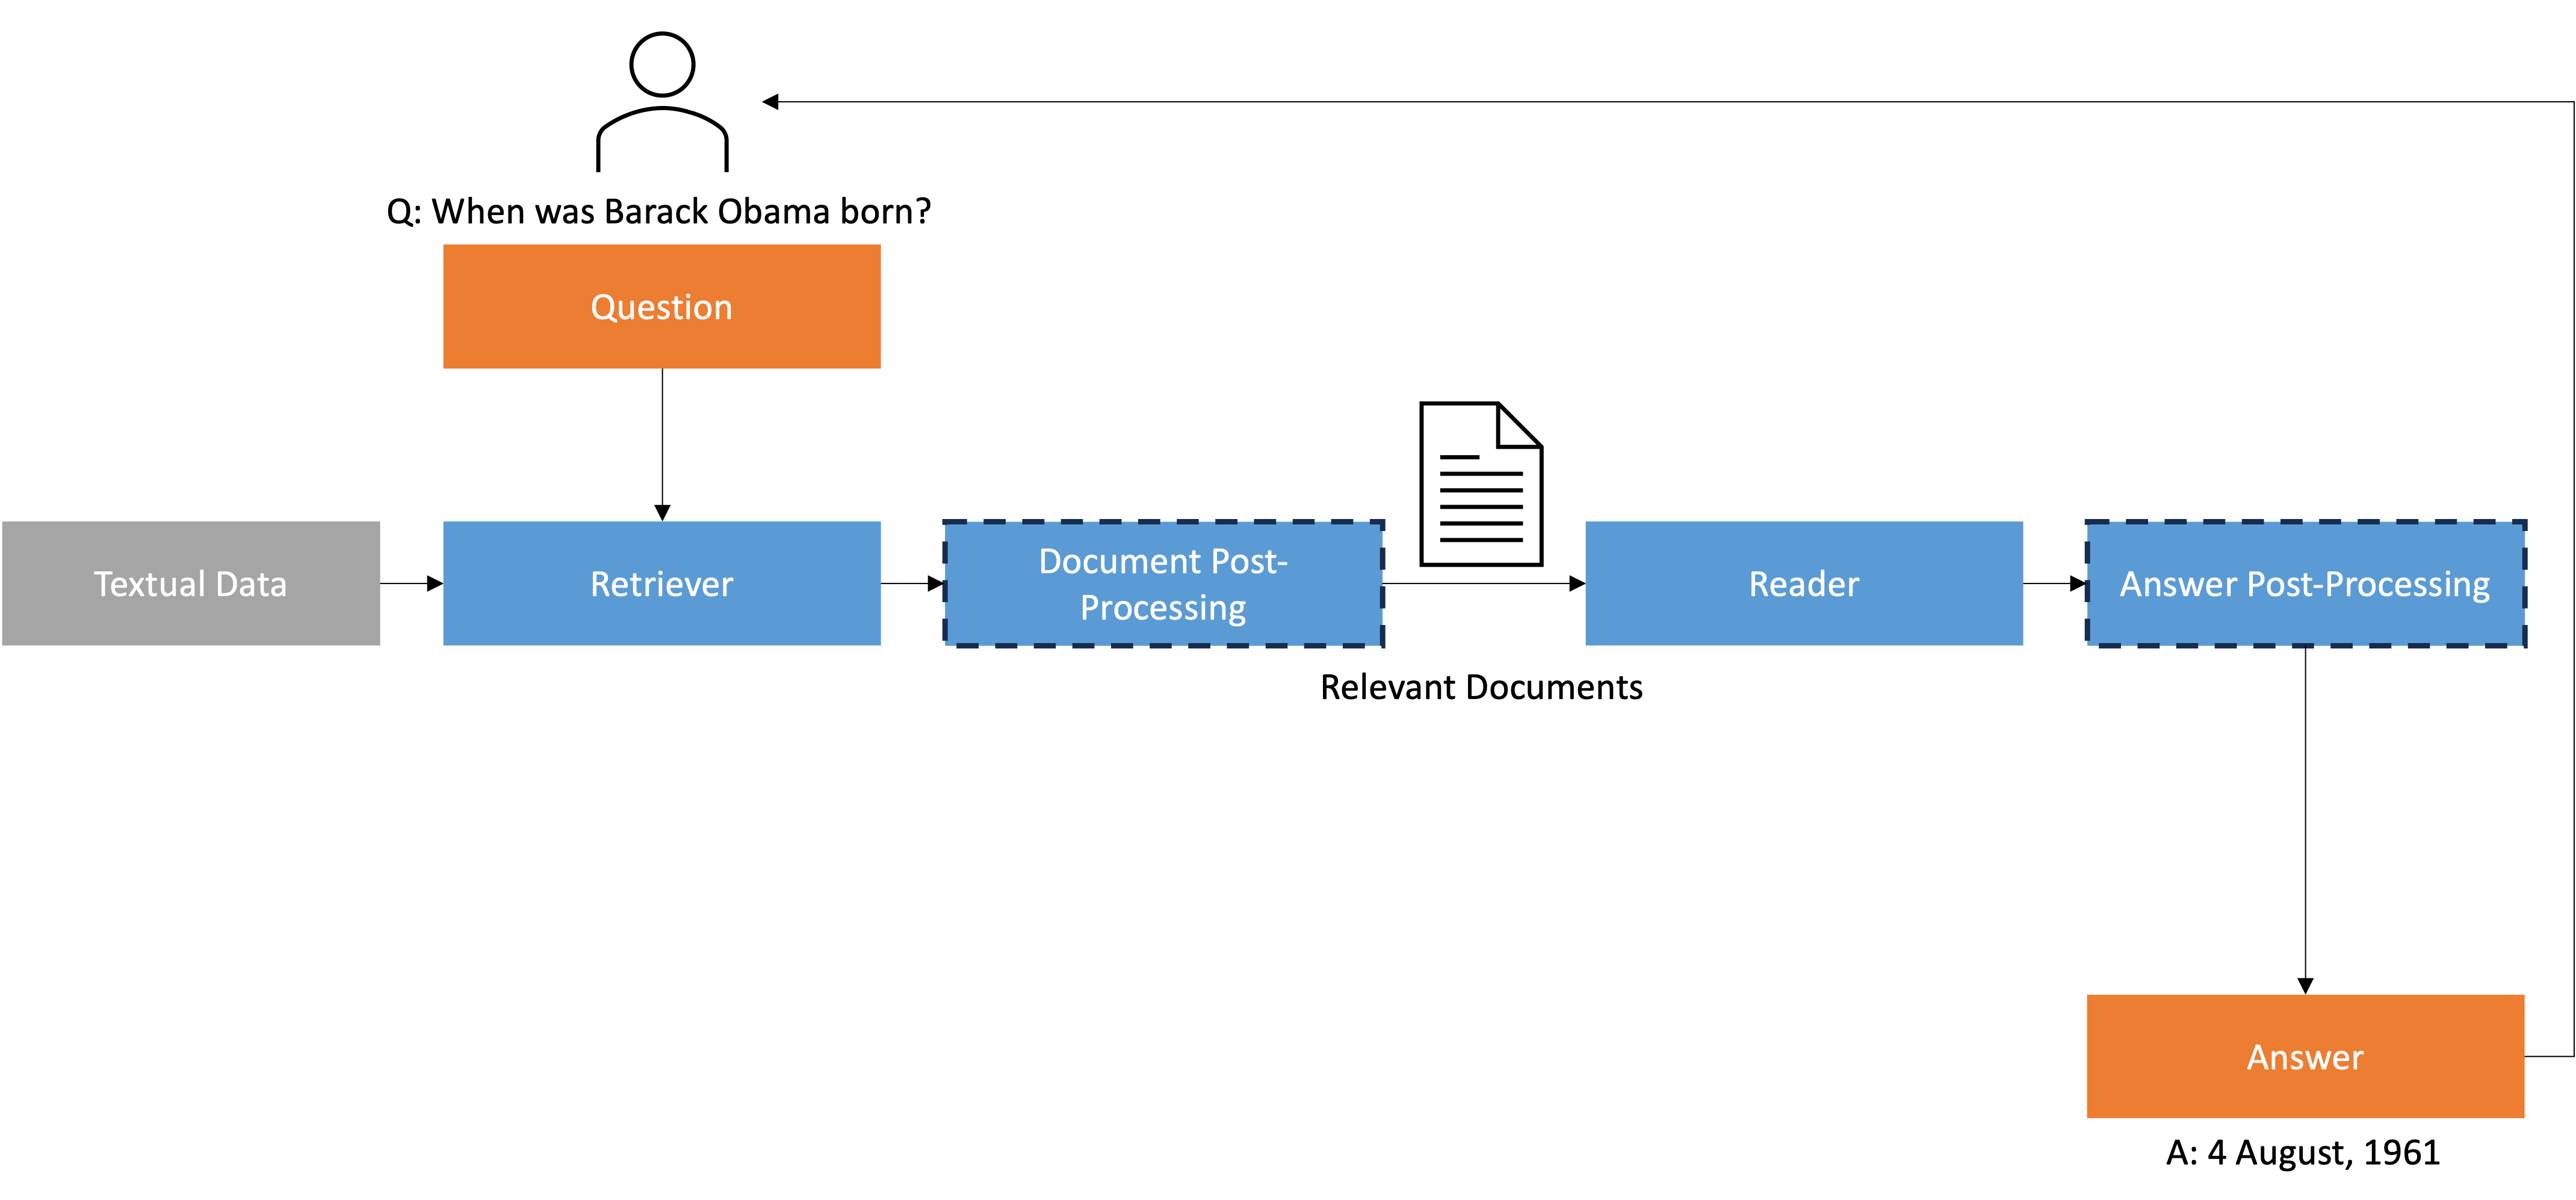
\includegraphics[width=\textwidth]{Grafiken/Retriever_Reader.png}
    \caption{Reader-Retriever-System Architecture for \gls{qa} by Zhu et. al. \cite{zhu_retrieving_2021}. The dashed lines indicate optional modules.}
    \label{fig:rr_architecture}
\end{figure}

Figure \ref{fig:rr_architecture} depicts the general architecture of a \textbf{Retriever-Reader-System}, as defined by Zhu et al. \cite{zhu_retrieving_2021}. This architecture serves as the foundational framework for \gls{ir}-Based \gls{qa} systems and was initially introduced by Harabagiu et al. \cite{harabagiu_open-domain_2003}. In this framework, all modules operate independently, can be trained separately, and are subject to independent evaluation.

The \textbf{Retriever} module's primary role is to retrieve relevant documents, passages, or other pertinent information from a knowledge source and rank them based on their relevance to answering the user's query. Subsequently, the \textbf{Reader} module extracts the answer from the retrieved documents and presents it to the user. This task bears a close resemblance to \gls{mrc}, with the key distinction that in \gls{ir}-Based \gls{qa}, the system must handle multiple documents and comprehend them to formulate a response, unlike classical \gls{mrc} tasks, which typically involve only one context document.

The \textbf{Document Post-Processor} module's role is to curate and refine the set of documents that will be forwarded as "Relevant Documents" to the subsequent stage, the Reader. Concurrently, the \textbf{Answer Post-Processor} assists the Reader in addressing complex questions for which the answer may not be found in a single document alone \cite{zhu_retrieving_2021,jurafsky_speech_2023}.

It's worth noting that some researchers include a \textbf{Question Analysis} module preceding the Retriever, which aims to preprocess the received question for more efficient query execution in the Retriever \cite{nassiri_transformer_2023}. However, for the purposes of this thesis, we adhere to Zhu et al.'s definition \cite{zhu_retrieving_2021}, where this functionality is considered part of the Retriever.

Conceptually, there are three distinct approaches to the Retriever itself: \textit{Sparse Retrieval, Dense Retrieval,} and \textit{Iterative Retrieval.} The specifics of these approaches will be thoroughly explored in Section \ref{subsec:qa_retrieval}.

Document Post-Processors can be categorized into \textit{Supervised Learning, Reinforcement Learning,} and \textit{Transfer Learning}-based approaches. A detailed discussion of these approaches is also provided in Section \ref{subsec:qa_retrieval}.

In Section \ref{subsec:qa_reader}, we will delve into the finer details of Reader approaches and Answer Post-processing. Broadly speaking, there are two primary types of Readers: \textit{Extractive} and \textit{Generative} Readers. As for Answer Post-processing, it involves two key categories: \textit{Rule-based} and \textit{Learning-based} approaches.

There are also \textbf{End-to-End} approaches that employ a single module to execute the entire \gls{qa} task. Excluding generative approaches, two common categories of such approaches are \textbf{Retriever-Reader} and \textbf{Retriever-only} models.

An End-to-End Retriever-Reader aims to train both the Retriever and Reader in a single backpropagation step, and in some cases, it introduces additional knowledge sources beyond the traditional \gls{ir} framework. An illustrative example is \gls{rag} \cite{lewis_retrieval-augmented_2021}. \gls{rag} consists of a pre-trained Generator with implicit knowledge encoded in its parameters and a pre-trained Retriever. For each question, the Retriever identifies the most relevant documents and generates a latent vector based on them. This latent vector, along with the original question, is fed into the Generator.

Another end-to-end approach, similar to \gls{rag}, is \gls{realm} \cite{guu_realm_2020}. While these previous two approaches extended the capabilities of pre-trained \gls{s2s} models, Nishida et al. pursued a different path by training a single \gls{nn} to perform both tasks simultaneously: \gls{ir} and \gls{mrc} \cite{nishida_retrieve-and-read_2018}.

It is noteworthy that all these end-to-end approaches have demonstrated competitive performance compared to state-of-the-art methods on specific \gls{qa} datasets.

An essential yet often underestimated question is: What defines textual data, and how should one preprocess formats such as PDFs to extract this textual content? While many datasets already comprise small contextual snippets \cite{wang_modern_2022}, it's crucial not to overlook the entire process of extracting snippets from unstructured PDFs, for example. Approaches to tackle this challenge will be explored in detail in the upcomming Section \ref{subsec:qa_indexing}.

% 2nd push

\subsection{Extraction Approaches}
\label{subsec:qa_indexing}

As discussed in the previous Section \ref{subsec:qa_basics}, the knowledge source for a \gls{qa}-System can take the form of textual or multimodal data. The specific type of data may necessitate certain requirements or specific adjustments to the Retriever used for \gls{ir}.

In the context of this thesis, the primary knowledge source to be employed is PDF documents. In the research field, three major approaches exist for extracting textual information from unstructured data types like PDFs: \textit{visual} \cite{tito_document_2021}, \textit{direct} \cite{wang_multi-passage_2019}, and \textit{alternative} \cite{dasigi_dataset_2021} extraction methods.

It's important to note upfront that the chosen extraction method is intricately connected to the subsequent retrieval approach. The specifics, including metadata alongside pure textual data and quality requirements, may vary among different extraction and retrieval methods.

The visual approach is closely aligned with the research field of \textit{Document Question Answering}. A well-known example dataset in this field is \gls{docvqa} \cite{tito_document_2021}. The primary concept behind the visual approach to document question answering is to capture not only the text of a PDF but also additional information such as the document's structure, various hierarchies on a page (e.g., sections, subsections), and the ability to analyze tables and figures. These hierarchical structures can be leveraged to create two-stage retrieval approaches. In these approaches, initially, a collection of relevant files is identified based on higher-level attributes like the document's title and abstract. Subsequently, a more granular retrieval process is executed over lower-level attributes such as passages within the relevant files. These \textit{Iterative Retrievers} will be further discussed in Section \ref{subsec:qa_retrieval} \cite{liu_dense_2021}.

The challenge of \textit{Visual Document Question Answering} typically involves taking images of PDF pages as inputs and mapping question-answer pairs to them. The answers are extracted from either a single paragraph or a combination of multiple paragraphs \cite{mathew_document_2021}. Nonetheless, the extraction pipeline in this case usually resembles the \textit{Retriever-Reader} architecture, where the extracted information from the visual processing is fed into such a system afterward. Researchers in this field often employ a pipeline that includes a \textit{Document Layout Analysis} model, followed by the application of an \gls{ocr} tool to the detected regions \cite{mcdonald_detect_2022}. Examples of a \textit{Document Layout Analysis} model include the Document Image Transformer by Li et al. \cite{li_dit_2022}.

The direct approach is the most prevalent method in the field of Question Answering (\gls{qa}) and Information Retrieval (\gls{ir}). The primary concept behind this approach is to extract textual information from PDFs and store it in a database. The extraction process can be accomplished using various tools such as \textit{PDFMiner} or \textit{Adobe Extract} \cite{meuschke_benchmark_2023}. However, a lingering question is how to effectively split the extracted textual data, especially considering that they are often not cleaned after extraction.

A common practice when employing a Language Model (\gls{llm}) is to optionally cleanse the text corpus and then divide it based on a predefined token size. This approach is evident in two notable open-source LLM projects: \textit{Langchain} and the \textit{Retrieval Plugin for ChatGPT} by OpenAI \cite{noauthor_langchain-ailangchain_nodate,noauthor_chatgpt_2023}. In the original Dense Retrieval paper by Karpukhin et al., a sliding window of token size 5 was utilized \cite{karpukhin_dense_2020}. Therefore, it can be assumed that for contemporary LLM applications, the precise quality of the data, ensuring that a document contains syntactically correct sentences, may not be as critical.

Apart from modern approaches involving text clipping, previous methods aimed to identify paragraphs and similar structures within the extracted texts \cite{zhu_retrieving_2021}.

An alternative approach involves the methodology employed in constructing the QASPER dataset. In this case, the authors conducted a pre-filtering of scientific papers' PDFs, selecting only those with freely accessible LaTeX files. They then utilized the S2ORC tool to extract cleaned textual data from these LaTeX files \cite{dasigi_dataset_2021}. It's important to note that this approach is highly specific to the QASPER dataset and cannot be universally applied. Nonetheless, it serves as an illustration of alternative methods for extracting textual data from PDFs.

% Commit #3

\subsection{Retrieval Approaches}
\label{subsec:qa_retrieval}

The traditional state-of-the-art in \gls{ir} relies on \textbf{Sparse Retrievers}, with one notable example being BM25. BM25 is renowned as "one of the most empirically successful retrieval models and is widely used in current search engines" \cite{zhu_retrieving_2021}. Nandan et al. even demonstrated that on modern \gls{odqa} datasets, BM25 remains a viable baseline for zero-shot \gls{ir} \cite{thakur_beir_2021}.

BM25 was originally introduced by Robertson et al. \cite{robertson_probabilistic_2009}. It operates by utilizing the TF-IDF token weights between a question $q$ containing tokens $q_1, \ldots, q_T$ and a set of passages $P$, where $p \in P$.

\begin{equation}
    \mathbf{s}_{q, p}^{\text{BM25}}=\sum_{i=1}^T \log \left(\frac{|\mathcal{P}|}{N\left(q_i, \mathcal{P}\right)}\right) \frac{n\left(q_i, p\right)\left(k_1+1\right)}{k_1\left(1-b+\frac{b|p|}{a v p l}\right)+n\left(q_i, p\right)}
    \label{eq:bm25}
\end{equation}

    
Equation \ref{eq:bm25} illustrates the BM25 score for a question $q$ and a passage $p$. In this equation, $N\left(q_i, \mathcal{P}\right)$ represents the count of passages in $\mathcal{P}$ that contain the token $q_i$, while $n\left(q_i, p\right)$ indicates the frequency of token $q_i$ within the passage $p$. The variable $|p|$ signifies the length of passage $p$, and $avpl$ stands for the average passage length in $\mathcal{P}$. The parameters $k_1$ and $b$ are free parameters, typically set to $k_1 = 0.9$ and $b = 0.4$ \cite{mcdonald_detect_2022,robertson_probabilistic_2009}.

Traditionally, this lexical Information Retrieval (\gls{ir}) approach has been capable of providing satisfactory retrieval results. However, in 2020, Karpukhin et al. demonstrated for the first time that a \textbf{Dense Retrieval} approach could outperform the Sparse Retrieval approach across multiple \gls{odqa} datasets \cite{karpukhin_dense_2020}. Consequently, the search for a general Dense Retrieval model has been ongoing, as these Dense Retrieval approaches offer advantages such as semantic matching and the ability to handle lengthy documents \cite{zhu_retrieving_2021}.

In general, there are three types of Dense Retrieval approaches \cite{zhu_retrieving_2021}: the \textbf{Representation-based Retriever}, often referred to as the \textit{dual-encoder} \cite{karpukhin_dense_2020}; the \textbf{Interaction-based Retriever}, often referred to as the \textit{cross-encoder}; and the \textbf{Representation-interaction Retriever}, often referred to as the \textit{multi-stop retriever}. Figure \ref{fig:types_of_retriever} illustrates the general architecture of these three types of Dense Retrievers.

The \textbf{Dense Passage Retriever (DPR)} by Karpukhin et al. serves as a notable example to explain the \textbf{Representation-Based Retriever}. Given a collection $M$ of text passages $p$ and a question $q$, the objective of DPR is to identify the $k$ most similar passages to the question. To achieve this, DPR employs two distinct \textbf{BERT} \cite{devlin_bert_2019} Encoders. One Encoder, denoted as $E_Q(\cdot)$, encodes the question $q$ into a $d$-dimensional vector, where $d = 768$. The other Encoder, labeled as $E_P(\cdot)$, encodes the passage $p$ into a $d$-dimensional vector at the \verb|[CLS]| token. The similarity between these two vectors is computed using the inner product:


\begin{equation}
    \mathbf{s}_{q, p}^{D P R}=\mathbf{E}_{Q}(q)^{\top} \mathbf{E}_{P}(p)
    \label{eq:dpr}
\end{equation}

The choice of the inner product as the similarity function is motivated by its computational efficiency and the demonstrated, comparable performance \cite{karpukhin_dense_2020}. It is crucial for the dot-product to yield a small value for pairs of questions and passages that are genuinely related. The training dataset $D$ comprises $m$ instances, where $q_i$ represents the question, $p_i^+$ denotes the positive passage, and $p_{i,n^-}$ represents the negative passage:

\begin{equation}
    \mathbf{D}=\left\{\left(q_{i}, p_{i}^{+}, p_{i, 1}^{-}, \ldots, p_{i, n}^{-}\right)\right\}_{i=1}^{m}
\end{equation}

The loss function is optimized using the negative log likelihood of $p_i^+$:

\begin{equation}
    \mathcal{L}_{D P R}=-\log \frac{\exp \left(\mathbf{s}_{q_i,p_i^{+}}^{D P R}\right)}{\exp \left(\mathbf{s}_{q_i,p_i^{+}}^{D P R}\right) + \sum_{j=1}^{n} \exp \left(\mathbf{s}_{q_i,p_{i,j}^{-}}^{D P R}\right)}
\end{equation}

It's important to note that in \cite{karpukhin_dense_2020}, the selection of negative passages was not arbitrary. Instead, two additional approaches were employed: BM25 top passages that do not contain the answer and positive passages paired with other questions.

One significant advantage of the Representation-Based Retriever is that passages can be pre-indexed locally rather than at runtime. This reduction in latency between the question and the response may, however, come with trade-offs in the quality of the retrieved passages.

The \textbf{Interaction-Based Retriever} incorporates both the question $q$ and the passage $p$ within a single model, separated by a \verb|[SEP]| indicator. These models offer various approaches for modeling the relationship between $q$ and $p$. For instance, one common method is to utilize the \verb|[CLS]| classifier as an indicator of whether the passage is relevant to the question. This approach was first introduced with \gls{bert} \cite{devlin_bert_2019}. While these models perform competitively with previous Representation-Based Retrievers, it's important to note that they are 100-1000 times more computationally expensive \cite{khattab_colbert_2020}.

To address this latency issue, models like ColBERT introduced the concept of \textbf{co}ntextualized \textbf{l}ate ineraction \cite{khattab_colbert_2020}. In this thesis and subsequently in research, it is referred to as the \textbf{Representation-Interaction Retriever} \cite{zhu_retrieving_2021}.


\begin{figure}
    \centering
    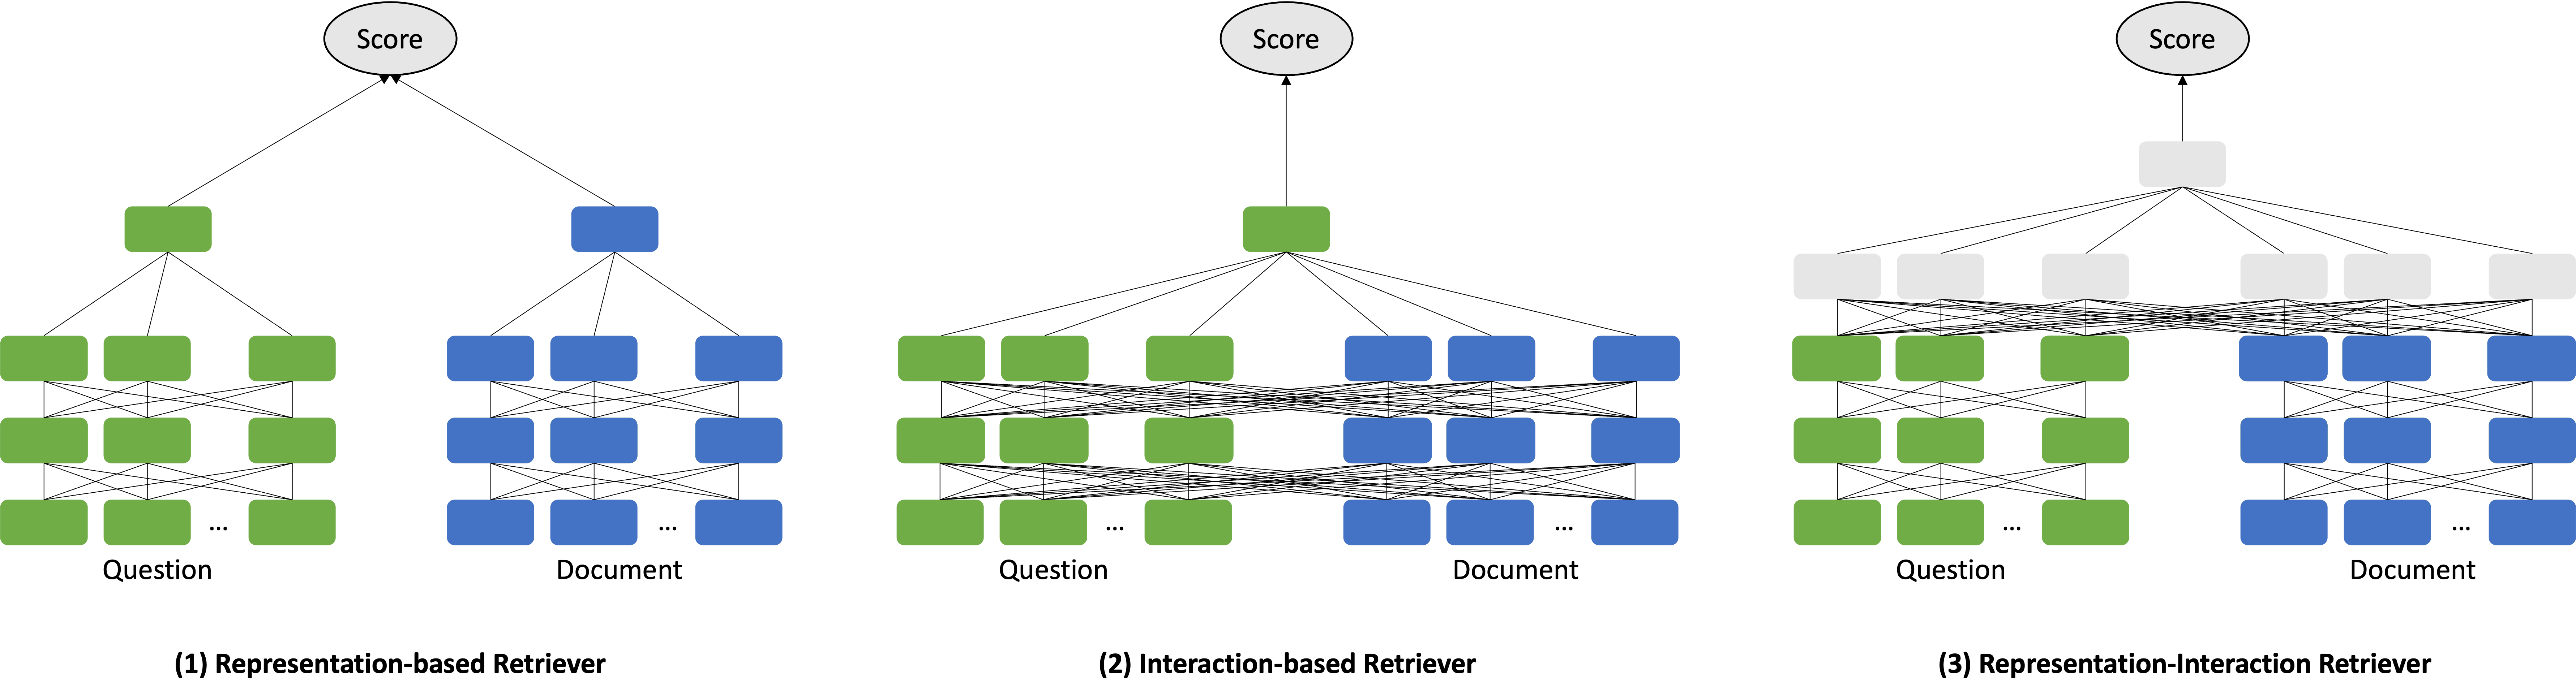
\includegraphics[width=\textwidth]{Grafiken/Types_of_Retriever.png}
    \caption{Types of Dense Retriever by Zhu et. al. \cite{zhu_retrieving_2021}.}
    \label{fig:types_of_retriever}
\end{figure}

ColBERT, like \gls{dpr}, employs two \gls{bert} Encoders, denoted as $E_Q\left(\cdot\right)$ and $E_P\left(\cdot\right)$. However, it introduces a late interaction mechanism. When provided with a query $q$, it is initially tokenized into BERT-based Wordpiece tokens, resulting in $q_1, \ldots, q_T$. Following the \verb|[CLS]| token, a \verb|[Q]| token is appended to signify the question. If the length of the tokenized question is less than $N_q$, a predetermined token length, the remaining portion of the question is padded with BERT's \verb|[mask]| token. Otherwise, it is truncated. This process, known as *query augmentation*, allows BERT to re-weight existing terms or expand the query, and it is pivotal to ColBERT's performance. The generated embeddings are then passed through a linear layer to reduce the output dimensions to a fixed size $m$, which is smaller than the original dimensions of BERT. The output is subsequently normalized to ensure that the L2 norm of each result equals one.

For each passage $p$, $E_P\left(\cdot\right)$ is employed for encoding. Similar to the question encoding process, $p$ is segmented into its $p_1, \ldots, p_{T_d}$ Wordpiece tokens. The special token \verb|[D]| indicates a passage. Short passages are not padded with a \verb|[mask]| token. After the classical BERT output, a similar post-processing step is applied to the encoded passages, and all embeddings corresponding to punctuation are filtered out.

\begin{equation}
    \mathbf{E}_{q}:= Normalize(CNN(BERT("[Q] q_0 q_1 \dots q_T [mask] \dots [mask]")))
\end{equation}

\begin{equation}
    \mathbf{E}_{p}:= Filter(Normalize(CNN(BERT("[D]p_0 p_1 \dots p_T"))))
\end{equation}

The late interaction mechanism applied to the encodings involves computing the maximum similarity, which utilizes cosine similarity through dot-products. This is made possible by the earlier normalization applied to the embeddings:

\begin{equation}
    \mathbf{s}_{q, p}^{C o l B E R T}=\sum_{I\in\left[\left|\mathbf{E}_q\right|\right]}\max _{j\in\left[\left|\mathbf{E}_d\right|\right]} \mathbf{E}_{q, i} \cdot \mathbf{E}_{p, j}^{\top}
\end{equation}

The interaction mechanism has no trainable parameters. ColBERT is differentiable end-to-end. During training, for example, with a triple $(q, p^+, p^-)$, ColBERT independently produces a score for each passage and is subsequently optimized pairwise using softmax cross-entropy loss over the scores of $p^+$ and $p^-$ \cite{khattab_colbert_2020}.

Another type of Retriever is the \textbf{Iterative Retriever}. Iterative Retrievers are necessary when dealing with questions that are more complex than simple factoid questions, which can be answered by identifying the right passage in the knowledge source. An example is the HotpotQA dataset \cite{yang_hotpotqa_2018}, designed specifically for multi-hop questions. The fundamental concept here is that such questions cannot be answered with just one precise piece of evidence. They require multiple passages from different documents at the very least. Iterative Retrievers encompass three stages in the pipeline: (1) document retrieval, (2) query reformulation, and (3) retrieval stopping.

An example is BEAM, currently holding the title of the highest-performing\footnote{Status as of September 23, 2023, according to https://paperswithcode.com and the authors of \cite{zhang_beam_2023}}, \gls{qa}-System across multi-hop \gls{qa} datasets such as HotpotQA \cite{zhang_beam_2023}. The document retrieval component can take the form of any retrieval model, including options like ColBERT, BM25, or \gls{dpr}. In the case of BEAM, it leverages an Interaction-Based Retriever using DeBERTa. For each candidate passage $p_c$, BEAM calculates a relevance score concerning this passage within the context of all previously identified relevant passages $p_r$ and the question $q$, using the embeddings of the \verb|[CLS]| tokens \cite{he_deberta_2020}. The second step, query reformulation, can be executed explicitly or implicitly, meaning it can either be expressed in natural language or as a dense embedding. The advantage of using natural language lies in its interpretability, while employing dense embeddings operates within a semantic space and does not lack vocabulary interpretability \cite{zhu_retrieving_2021}. BEAM adopts a natural language-based approach. Specifically, after each hop, it appends the newly identified passage to the previously identified ones and feeds this information into DeBERTa.

\begin{equation}
    \text{s}_{q, p}^{BEAM} = \text{Classifier}(\text{DeBERTa}("[CLS] q \: p_{r_1} \: \ldots \: p_{r_i} \: ")) \quad | \quad p_{c} \in P
\end{equation}

The nature of query reformulation depends on the type of retriever in use. Lastly retrieval stopping poses its own set of challenges. A common approach involves setting either a fixed number of hops or a maximum limit on the retrieved documents. Alternatively, some methods introduce a new token, such as \verb|[EOE]| (End-of-Evidence), to signal the end of retrieval \cite{zhu_retrieving_2021}. BEAM, for example, employs a fixed number of hops, specifically 2, as determined through empirical evaluation.

The task of \textbf{Document Post-Processing} is to reduce the number of passages forwarded to the Reader, aiming to eliminate irrelevant ones. Traditional Retrievers, like Sparse Retrievers, often required a Document Post-Processor. However, Dense Retrievers often incorporate ranking and retrieval simultaneously, rendering this module unnecessary \cite{zhu_retrieving_2021}. Nevertheless, it remains possible to construct multi-stage Retrievers to, for instance, increase latency. This can be achieved by using a simpler Dense Retriever for pre-filtering passages and subsequently applying a more accurate one \cite{liu_dense_2021}.

% Commit #4

\subsection{Reader Approaches}
\label{subsec:qa_reader}

Readers originally emerged from the field of \gls{mrc}, where the objective is to extract an answer from a given context. A well-known example is the SQuAD \cite{rajpurkar_squad_2016} dataset, which was mentioned in Section \ref{subsec:qa_basics}. However, unlike the original \gls{mrc} task, a Reader in a Retrieval-Reader-System must process multiple passages to determine the relevant information needed to answer a given question \cite{zhu_retrieving_2021}. 

Modern readers rely on \gls{prlm}s since they establish new baselines on well-known datasets \cite{luo_choose_2022}. In general, there are two types of Readers that use \gls{prlm}s: \textbf{Extractive Readers} and \textbf{Generative Readers} \cite{jurafsky_speech_2023,zhu_retrieving_2021,luo_choose_2022}.

In general, an \textbf{Extractive Reader} employs an encoder to identify the token sequence span that is relevant for answering a question. These encoders can be any autoencoder models, such as BERT \cite{devlin_bert_2019}, DeBERTa \cite{he_deberta_2020}, or RoBERTa \cite{liu_roberta_2019}. Luo et al. \cite{luo_choose_2022} even utilized the encoder components of established encoder-decoder models like T5 \cite{raffel_exploring_2023} and BART \cite{lewis_bart_2019}. They demonstrated that, after fine-tuning, these models can outperform encoder-only models on certain tasks.

Figure \ref{fig:extractive_reader} illustrates the span labeling process performed by the extractive reader. The question tokens $q_1, \ldots, q_n$ and the passage tokens $p_1, \ldots, p_m$ are input into the encoder, separated by a \verb|[SEP]| token. The encoder learns two new embeddings, $S$ and $E$, which represent span-start and -end tokens, respectively. To obtain the span start probability for an output token $p_i^{\prime}$, the dot product between the output token and $S$ is computed and then normalized by a softmax function over all output tokens. The process is similar for the span-end token. The score of a span from position $i$ to $j$ is calculated as $S * p_{i}^{\prime} + E * p_{j}^{\prime}$. The span with the highest score, where $j \geq i$, is selected as the answer span. If the total length of tokens in $q$ and $p$ exceeds the maximum input length of the encoder, the passage is split into multiple segments, and the process is repeated for each segment \cite{jurafsky_speech_2023,luo_choose_2022}.

\begin{figure}
    \centering
    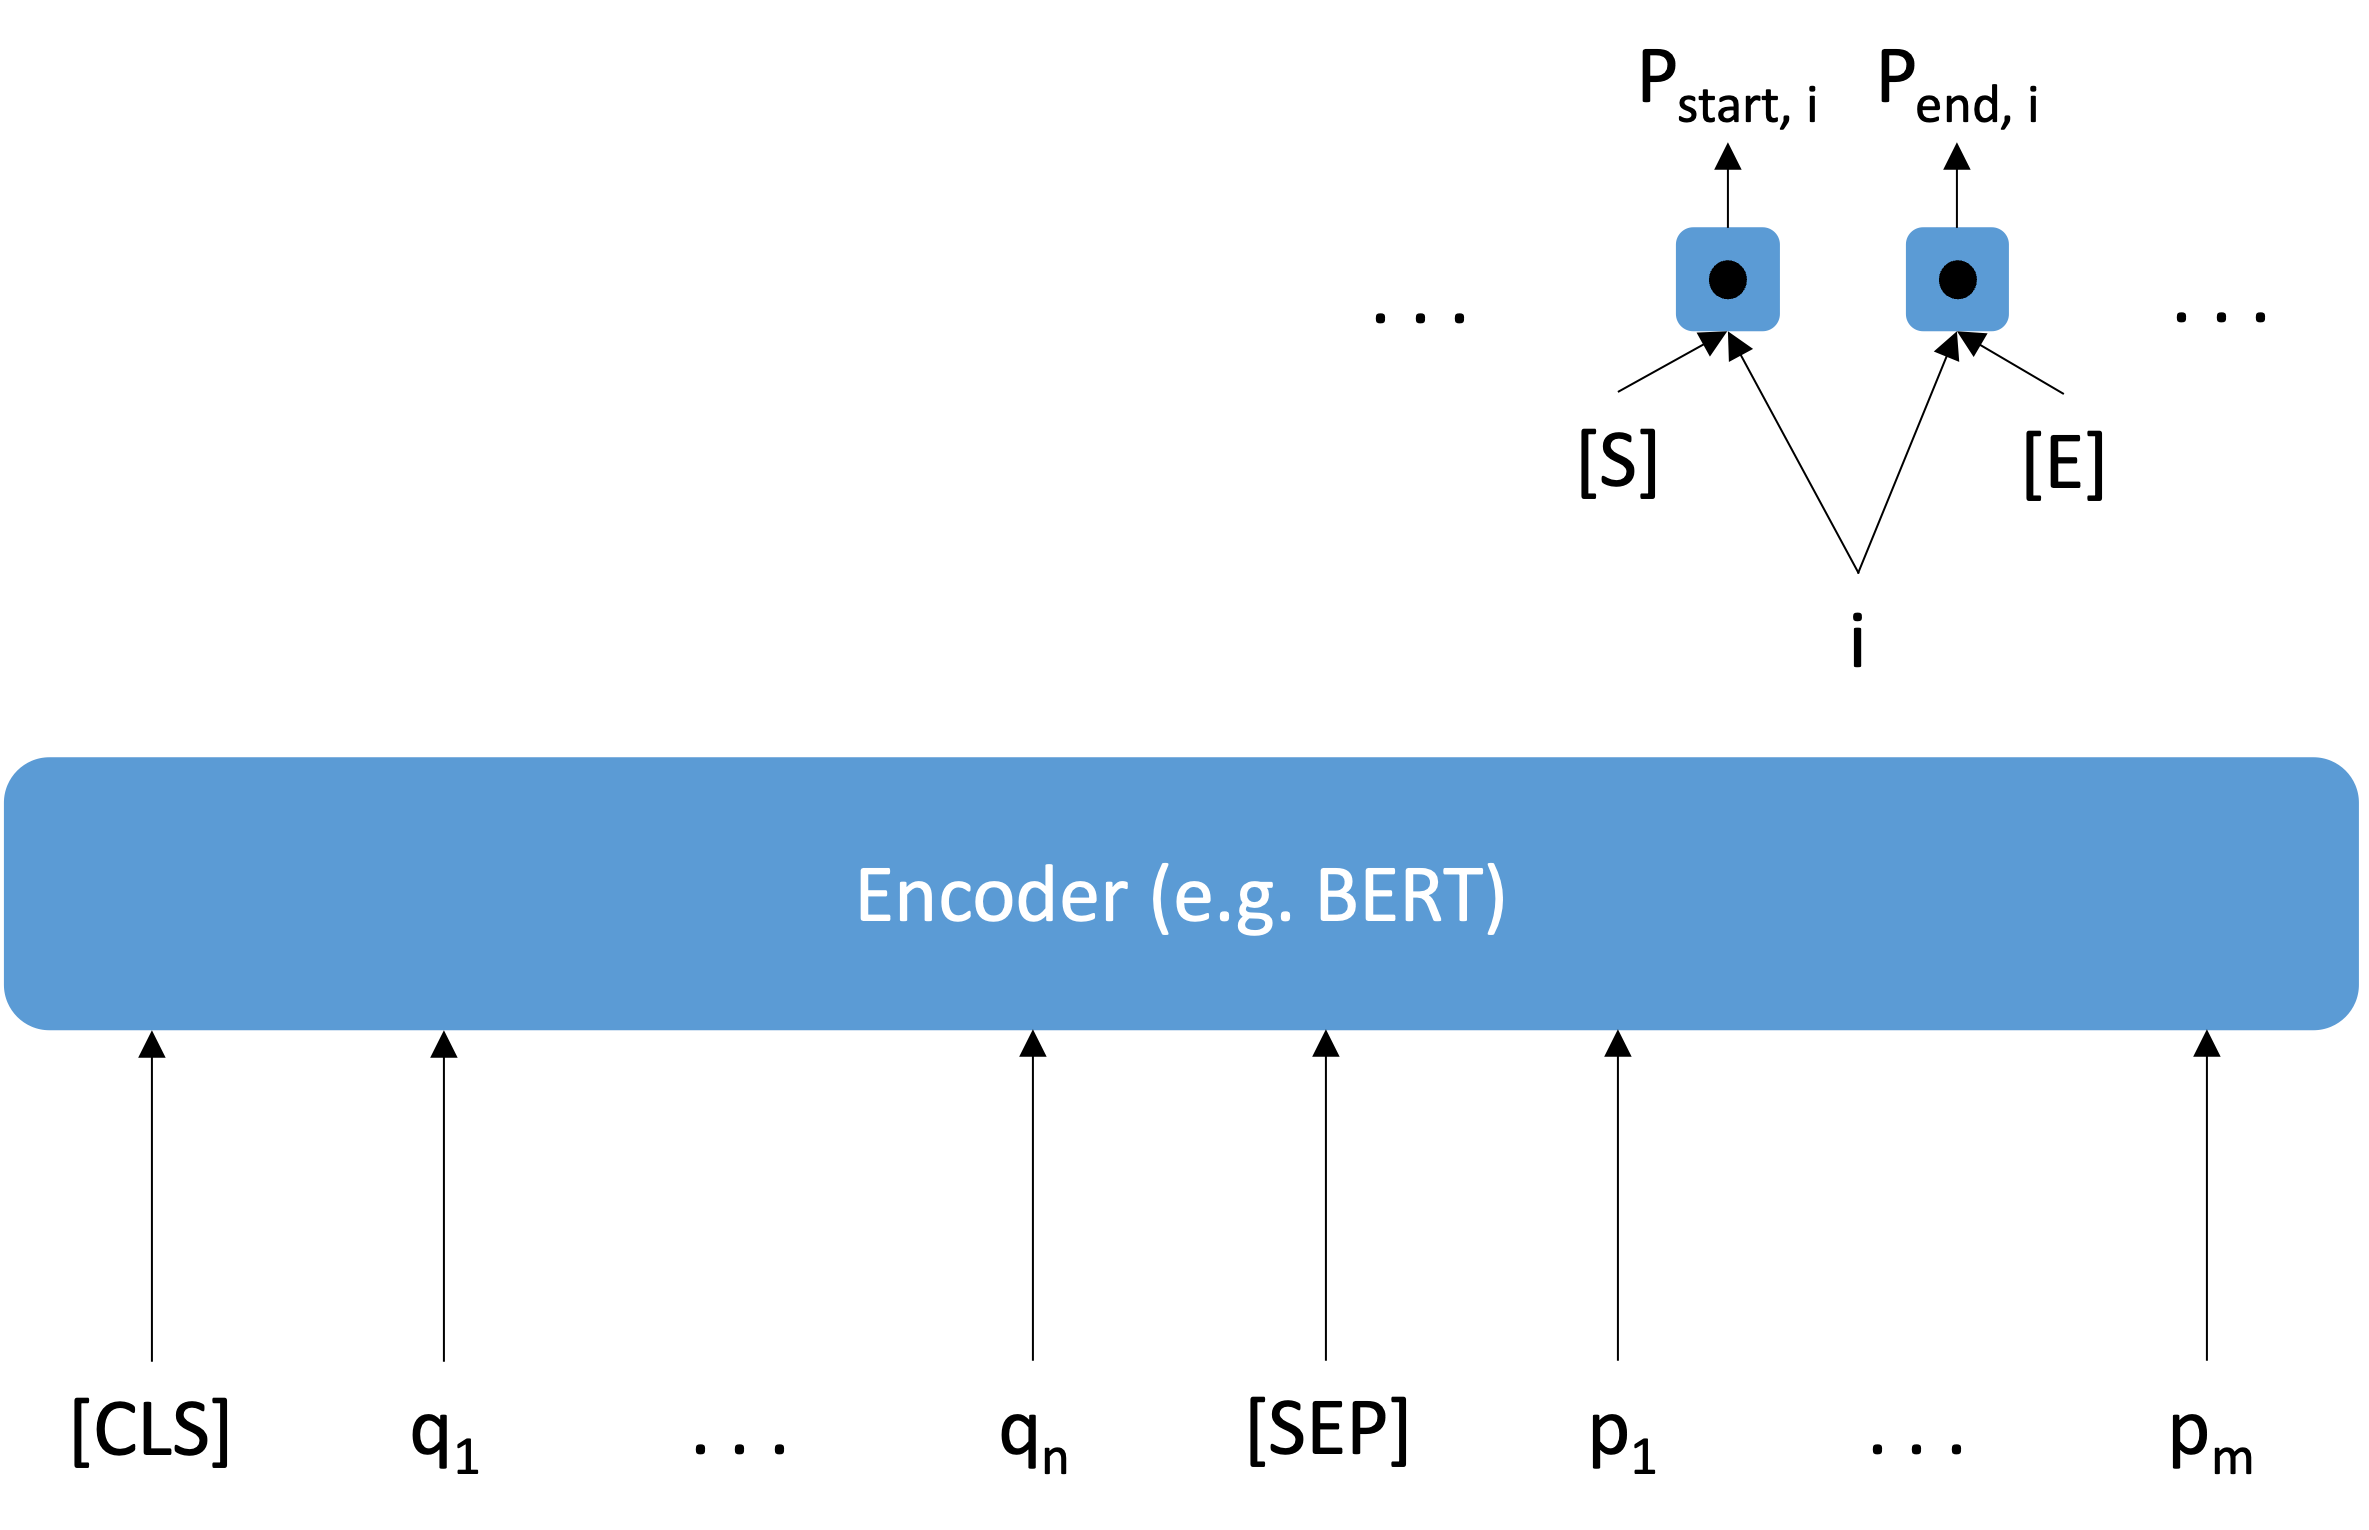
\includegraphics[width=\textwidth]{Grafiken/Extractive_Reader.png}
    \caption{Adjusted Graphic of the Extractive Reader by Jurafsky et al. \cite{jurafsky_speech_2023}}
    \label{fig:extractive_reader}
\end{figure}

The \textbf{Generative Reader} operates straightforwardly when familiar with a \gls{s2s} encoder-decoder model. Given a dataset containing $(q,p,a)$ tuples, the encoder takes $q$ and $p$ as input and outputs the contextual representation $h$. Then, it is the decoder's task to generate a token sequence based on $h$ and attention. The training objective can be described as minimizing the following loss function:

\begin{equation}
    \mathbf{\mathcal{L}_{\mathrm{Gen}}=\sum_{i=1}^K \log \mathbf{P}\left(a_i \mid \mathbf{h}, a_{: i}\right)}
\end{equation}

Here, $K$ represents the length of tokens in $a$, $a_i$ is the $i^{th}$ token in $a$, and $a_0$ is a special beginning of sequence token. In cases where the answer is not contained within the passages, the \verb|[CLS]| token indicates this situation \cite{luo_choose_2022,zhu_retrieving_2021}.

Latest research projects like Visconde \cite{pereira_visconde_2022} even employ \gls{llm} as Generative Readers. The performance and usability of these models remain active topics of research.

Luo et al. conducted the first survey comparing state-of-the-art Extractive and Generative Readers \cite{luo_choose_2022}. They discovered that \enquote{on average, extractive readers perform better than generative ones} \cite{luo_choose_2022}, except in cases involving long context passages, where generative approaches outperform the extractive ones.

The \textbf{Answer Post-Processor} is similar to the Document Post-Processor, serving as an optional component. Its primary task is to provide support for multi-hop complex questions, helping determine the final answer from a set of answers extracted by the reader component \cite{zhu_retrieving_2021}. Depending on the implementation of the Reader, this component may become obsolete.

% Commit #5

\subsection{Limitations}
\label{subsec:qa_limitations}

The evaluation metrics for \gls{ir} systems will be discussed in detail in Section \ref{chap:eval}. In general, selecting the components and models for an \gls{ir} system always involves a trade-off between accuracy, memory consumption, and inference speed \cite{zhang_survey_2023}.

Accuracy is primarily determined by the chosen Retriever-Reader-System. Sparse retrievers often lack a certain degree of semantic understanding, resulting in less accurate retrieved passages. In contrast, Dense Retrievers can achieve higher levels of accuracy but require thorough evaluation and training for the desired use case. Thakur et al. demonstrated that high-accuracy Dense Retrievers like \gls{dpr} can underperform in zero-shot scenarios compared to BM25 by -47.7\% \cite{thakur_beir_2021}. This highlights another crucial limitation of all \gls{nn}-based retrievers and readers: training. BM25 is, by nature, an unsupervised model for \gls{ir}, while common approaches for Dense Retrieval usually belong to the group of supervised models. These models heavily depend on their training data, whereas a Sparse Retriever like BM25 can be used without any training. According to experiments conducted by Thakur et al. \cite{thakur_beir_2021}, the best-performing out-of-distribution Retrievers are Representation-Interaction Retrievers like ColBERT.

Constructing a training dataset for a \gls{qa} task can be a tedious process, as these datasets must consist of tuples in the form of $(\text{question, context, answer})$, which is not always feasible. One established research direction to address this issue is \gls{qg} \cite{serban_generating_2016}. In \gls{qg}, a \gls{s2s} model is employed to generate questions and answers based on a given passage.

Zhang et al. provide an example of \gls{dpr} applied to the Natural Questions dataset in their survey on efficient \gls{odqa} \cite{zhang_survey_2023}. The total processing time for a query is 0.91 seconds\footnote{It's important to mention that \gls{dpr} is a Representation-based Retriever, which allows offline storage of passage embeddings. The result was obtained using an Nvidia GeForce Rtx 2080 Ti GPU, averaged over 1000 examples}. This time is divided into 74.79\% for evidence search and 23.95\% for reading. The total memory cost is 79.32GB, with the index occupying 81.95\%, the raw corpus 16.39\%, and the model 1.66\%. Approaches to optimize this may include:

\begin{enumerate}
    \item Reducing Processing Time: (1) Accelerating Evidence Search, (2) Accelerating Reading
    \item Reducing Memory Cost: (1) Reducing Index Size, (2) Reducing Corpus Size, (3) Reducing Model Size
    \item One-stage Frameworks: (1) Directly Generating Answers, (2) Directly Retrieving Answers
\end{enumerate}

Techniques used in this context may include:

\begin{enumerate}
    \item Data-based: (1) Passage Filtering, (2) Dimension Reduction, (3) Product Quantization
    \item Model-based: (1) Model Pruning, (2) Knowledge Distillation, (3) Knowledge Source 
\end{enumerate}

A common technique, which is used in nearly every experimental setup for \gls{qa}-Systems, is FAISS\cite{johnson_billion-scale_2017}, a GPU optimized implementation of the exact $k$-means clustering algorithm.

For a detailed overview of approaches towards more efficient \gls{odqa} systems, please refer to the comprehensive survey by Zhang et al. \cite{zhang_survey_2023}.

% Commit #6

\section{Conversational Question Answering}
\label{sec:cqa}

The differentiation of \gls{convqa} towards \gls{qa} will be discussed in Section \ref{subsec:cqa_basics}. This Section also introduces the fundamental concepts of \gls{convqa} which are necessary to understand challenges and necessary components compared to a regular \gls{qa}-System. Section \ref{subsec:cqa_contextual_query_understanding} will cover approaches towards the concept of query expansion. Section \ref{subsec:cqa_initiative} will clampse on the concept of initative and further approaches towards a Conversation Manager. Lastly Section \ref{subsec:cqa_llm_agents} will cover the usability of \gls{llm}s and especially the concept of Chain of Thoughts for \gls{convqa}.

\subsection{Basics}
\label{subsec:cqa_basics}

Core concepts in the field of \gls{odcqa} towards a conversation in terms of \gls{convqa} are: \textit{Turns}, \textit{Hisotry}, \textit{Memory}, \textit{Session} and \textit{Dialog Features} and \textit{Dialog State} \cite{zamani_conversational_2023}. It's important to mention, that in other subdomains/-tasks of \gls{cis} more concepts are introduced, such as \textit{State}, those are not necessary or applicable for \gls{odcqa} \cite{zaib_conversational_2021}.

Figure \ref{fig:conversation_explain} shows the core concepts based on a chat. Firstly, a \textbf{Turn} is a question-response pair. Whereas a conversation usually consists of multiple turns (multi-turn). \gls{coqa} is a dataset published in 2019 by researchers at Stanford in order to extend the known \gls{qa} dataset SQuAD towards a conversational dataset, whereas on average one conversation session consists of 15 turns \cite{reddy_coqa_2018}. Multi-turns are the main distinguisher betwenn the in Section \ref{sec:qa} introduced task, to a \gls{convqa} task. In a multi-turn scenario natural language phenomena like \textit{coreference} (multiple expressions refereing to the same thing) or \textit{ellipsis} (omitting words or topics implied by the context) can occur. While in regular \gls{qa} the System will only be challenged with single-turn scenarios, so only one question, which needs an answer, in \gls{convqa} the systems have to face multi-turn scenarios, where a user might also ask followup question or in general mutliple questions aftereachother. A \textbf{Hisotry} is consequently a set of turns which belong to one conversation session. A \textbf{Session} is a in it completed conversation. Lastly, the \textbf{Memory} is the abstract entity in which the \gls{convqa}-System stores knowledge related to a history, session or even user in general \cite{zamani_conversational_2023,gao_neural_2022}. This depends of the implementation of memory in the \gls{convqa} pipeline, which will be discussed in Section \ref{subsec:cqa_contextual_query_understanding}.

\textbf{Dialog Features} need to be assesed extra to the other mentioned concepts. While the other concepts tackle the conversations frame, the dialog feature evaluates the user questions themself. Possible dialog features may include: \textit{drilling-down} questions, \textit{topic-shift}, \textit{clarification} or \textit{definition}. Different dialog features call for different responses by the system \cite{gupta_conversational_2020}. The \textbf{Dialog State} has to be assesed similar. The dialog state represents the relation between turns. In cases of pre-defined domains methods like state slots are used, e.g. \verb |Date _, Location _, Artist _| have to be filled during the conversation in order to retrieve the correct information from the \gls{kb} \cite{rastogi_schema-guided_2020}. Open-Domain \gls{convqa} usually don't track the state \textit{explicitly}, but rather track it \textit{implicitly} via the type of implementation of the \textit{Contextual Query Understanding} unit.


\begin{figure}
    \centering
    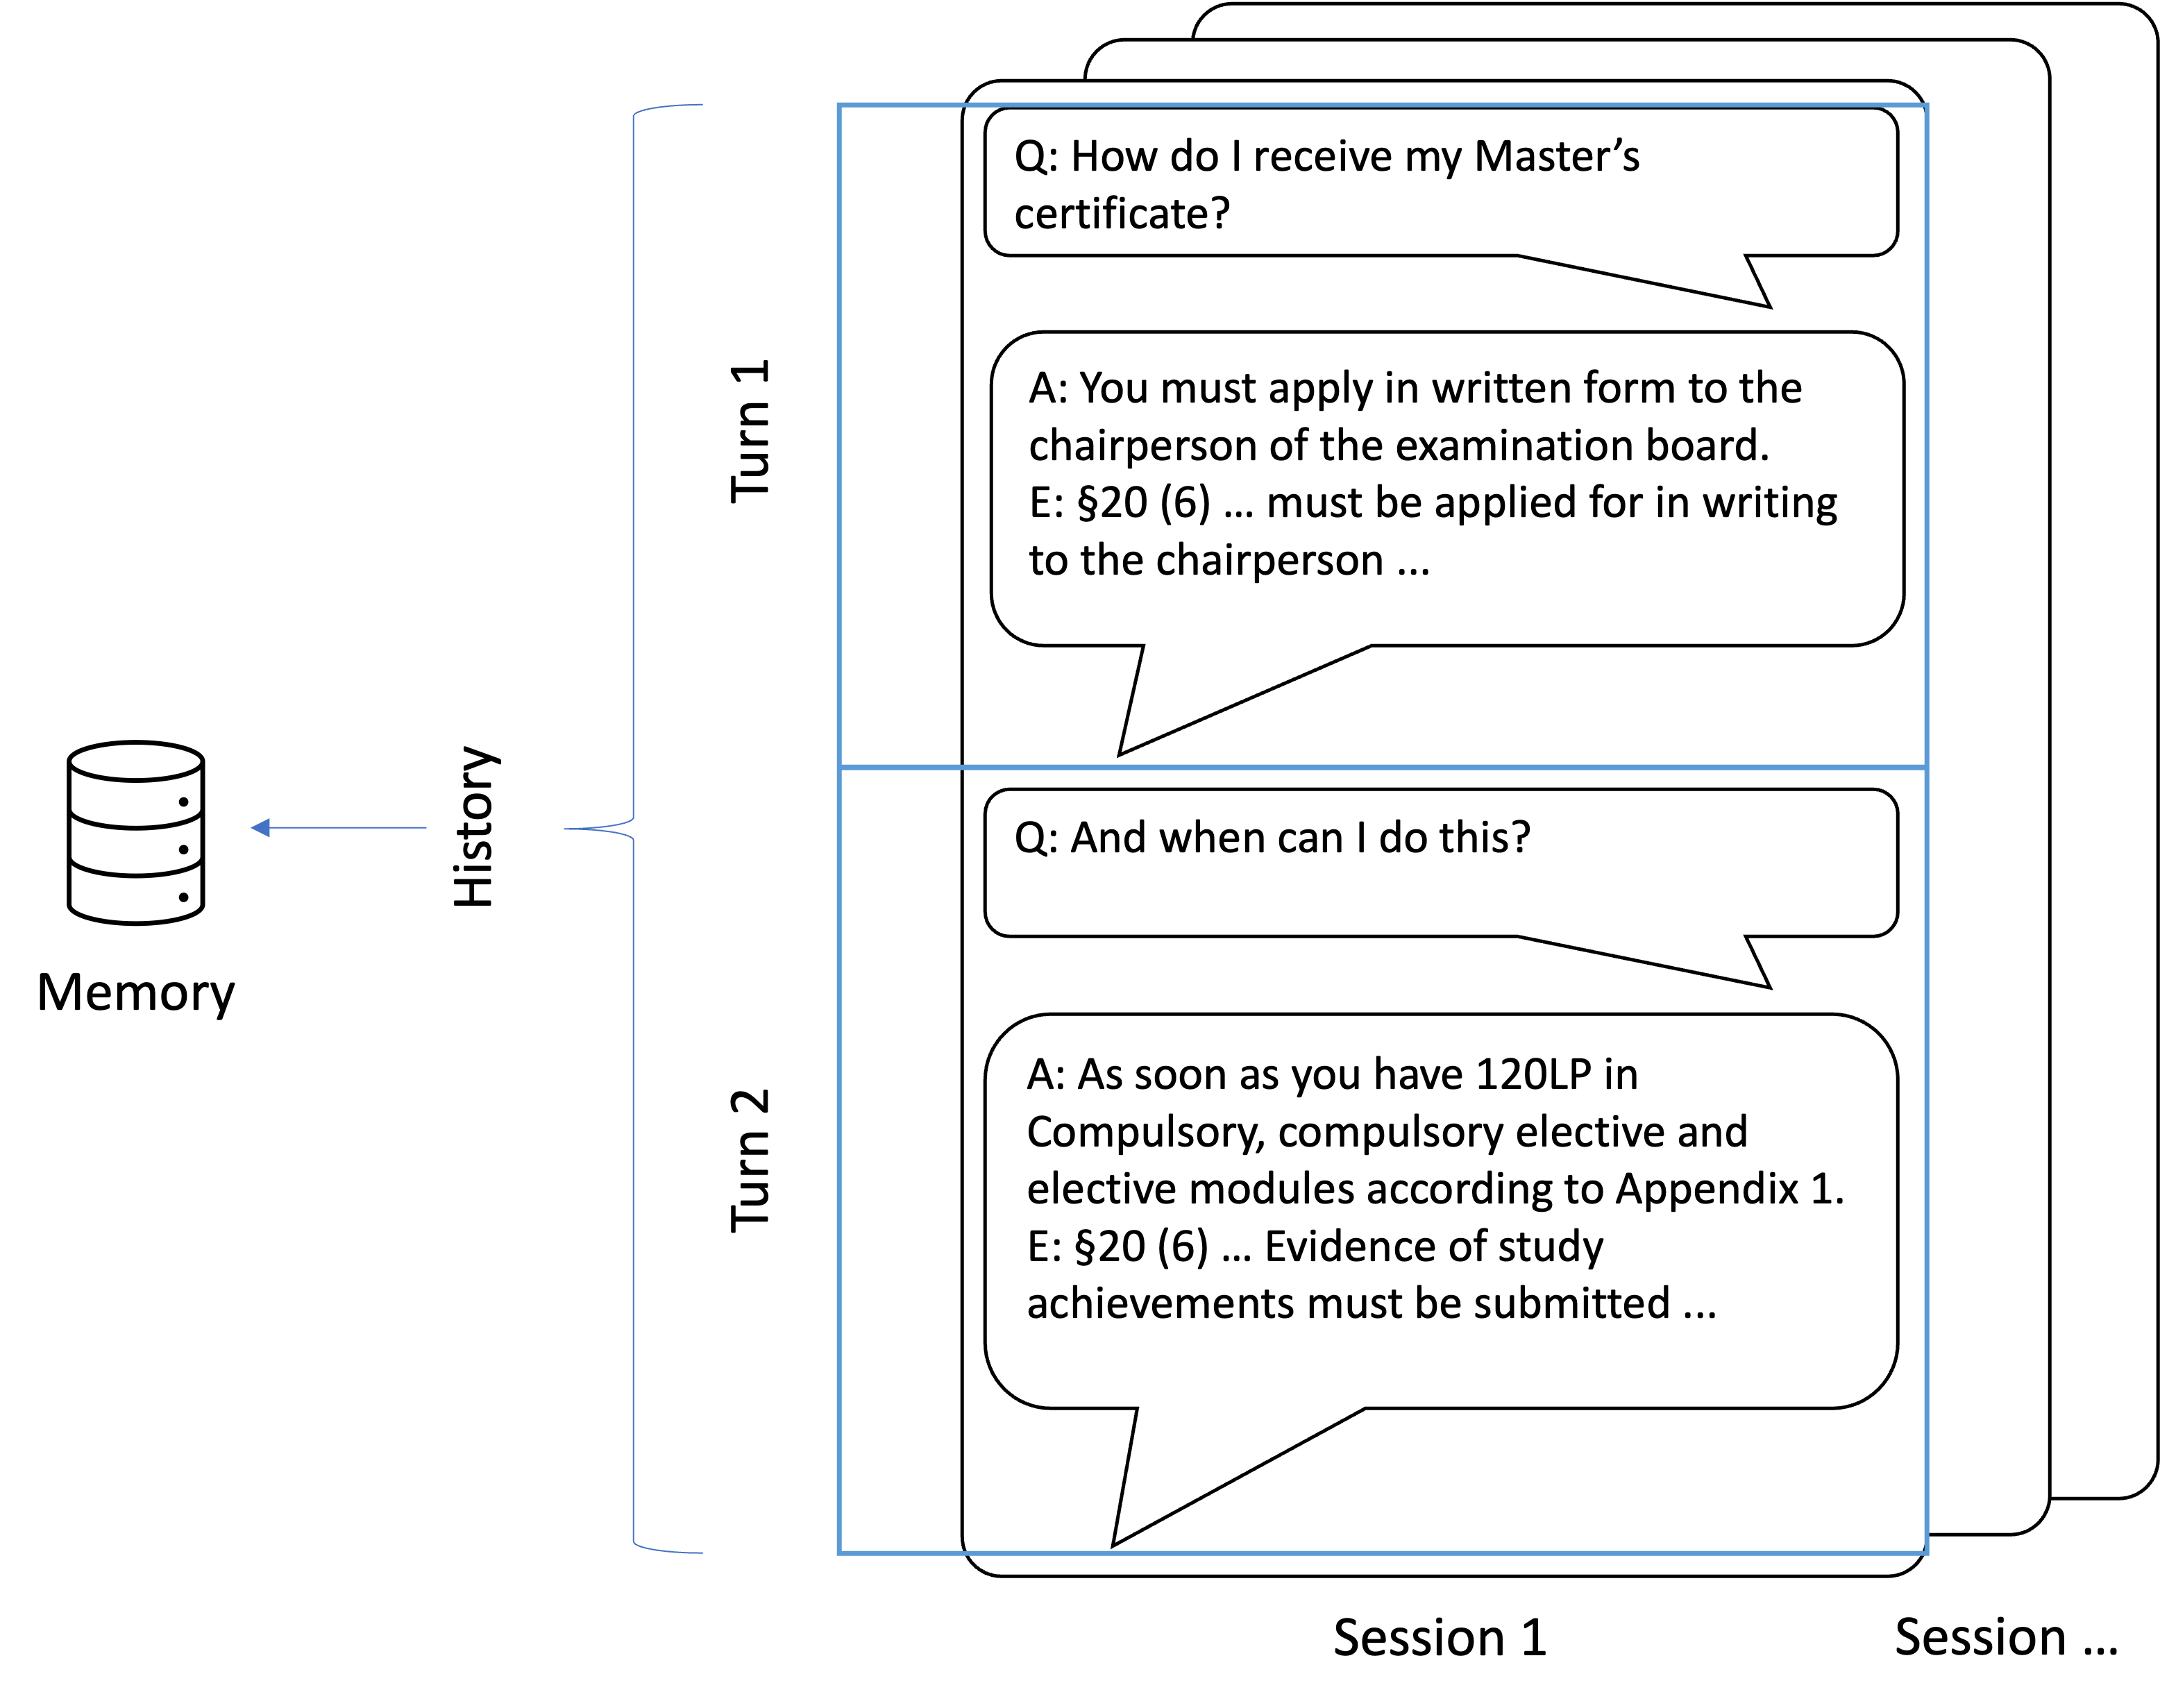
\includegraphics[width=\textwidth]{Grafiken/Conversation_Explain.png}
    \caption{Concepts of a Conversation in regards to a \gls{cis}}
    \label{fig:conversation_explain}
\end{figure}

Regarding the System architecture of a \gls{convqa} there is no one fits them all solution at the moment, but Gao et. al. \cite{gao_neural_2022} presented a modern system architecture, which represents commonly used appraoches and their corresponding components in a genral fashion. This general architecture can be observed in Figure \ref{fig:convqa_system_architecture}. Modern \gls{convqa} systems are closely realted to \gls{qa} systems, but lag certain generalizing components in order to be full \gls{cis} systems \cite{zamani_conversational_2023}.

\begin{figure}
    \centering
    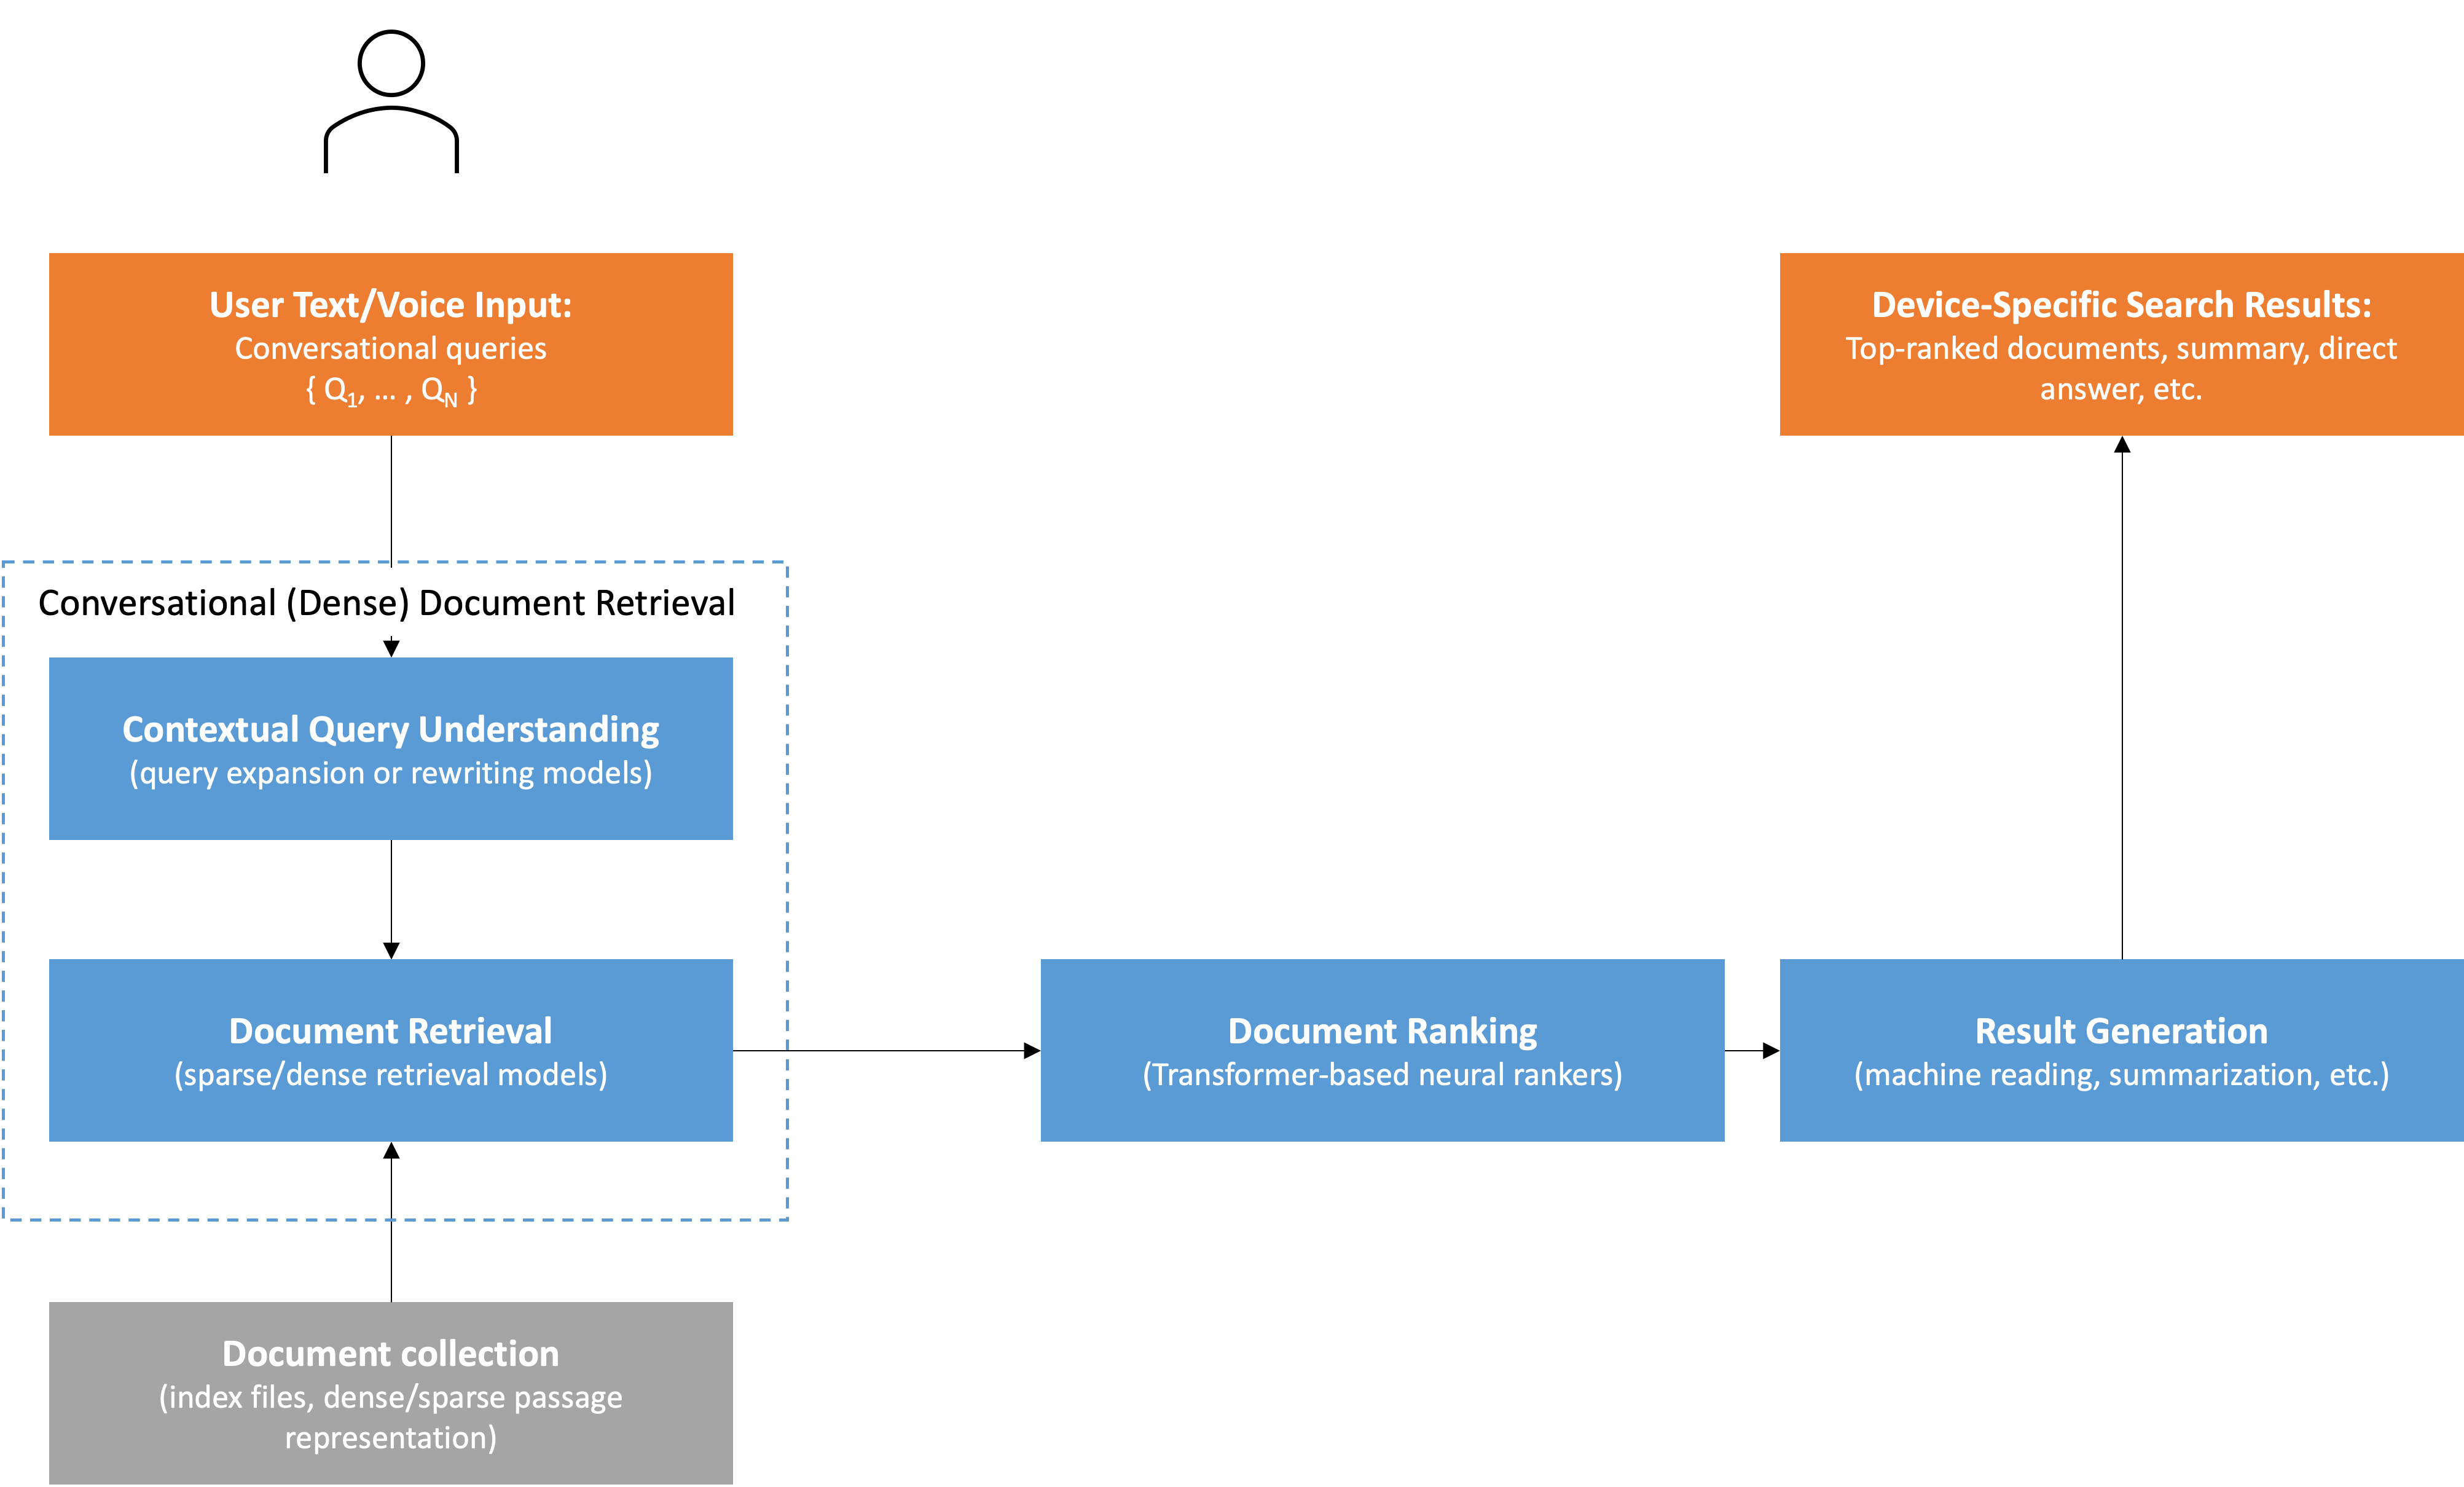
\includegraphics[width=\textwidth]{Grafiken/System_Architecture_ConQA.png}
    \caption{General System Architecture of a \gls{convqa} System by Gao et. al. \cite{gao_neural_2022}}
    \label{fig:convqa_system_architecture}
\end{figure}

Similar to the retriever-reader architecture introduced in Section \ref{subsec:qa_architectures}, a \gls{convqa} is made up of those two components as well, whereas in the case of a \gls{convqa} the retrieval as also the reader component have to handle more. The retriever has to understand the context, so the history of a conversation and retrieve based on that the most relevant documents. The reader on the other hand is close related to the reader of a classic retriever-reader architecture \cite{zamani_conversational_2023,gao_neural_2022}. Some implementations even feed into the reader component the context in order to rank the retrieved passages better and generate a more accurate answer \cite{owoicho_trec_2022}.

\subsection{Contextual Query Understanding}
\label{subsec:cqa_contextual_query_understanding}

How do we implement \textit{Memory}? Is the core question of this Section \ref{subsec:cqa_contextual_query_understanding}. 

There are two main distinguishing appraoches towards history implementation. The first is a simple heuristic of using the last-$k$ turns for \textbf{Query Expansion}, \textbf{Query Rewriting} or \textbf{Conversational Retrievers}. The second is to extract the important parts of the history in regards to a question and use them for Query Expansion or Rewriting \cite{gao_neural_2022}.

A good example to explain the appraoch of the second approach towards extracting improtant parts of the history $H = {(q_1, a_1), \dots , (q_i, a_i)}$ given a new question $q_{i+1}$ is \gls{quretec}\cite{voskarides_query_2020}. \gls{quretec} consits of two components essentially: one BERT-based model and a trainable classification layer. The $H$ is being passed through the BERT model, whereas the following structur of concatination is being used: 

\begin{equation}
    \text{BERT}([CLS],H,[SEP],q_{i+1}) 
\end{equation}

On every first sub-token of a term of the $H$ the term classification layer is applied, which is a network consisting of a dropout layer, a linear layer and a sigmoid function. The term classification layer predicts a label between $0-1$ indicating it's importance for answering the new question $q_i$. This leads to a set of terms $I$ which need to be incorporated into the retrieval \cite{voskarides_query_2020}. This is generaly also known as \textbf{Query Expansion}, whereas we add terms to a given query for retrieval. Next to this supervised, trained approach, there are also implementations which work unsupervised like Historical Query Expansion (HQExp) \cite{yang_query_2019}, which was one of the best performing models in the TREC CAsT 2019 \cite{dalton_trec_2020}.

Modern neural appraoches more often implement a \textbf{Query Rewriting} module which is build on top of \gls{s2s}-models to rewrite a query $q_{i+1}$ given a history $H$ in order to use the generated new query for retrieval using an established \gls{qa} retriever \cite{owoicho_trec_2022}. The main advantage of this appraoch is the abscence of the need of large supervised datasets as for Conversational Retrievers \cite{dai_dialog_2022}. One of the top performing models in the TREC CAsT 2022 was HEATWAVE by a Team of the University of Cambridge England \cite{liusie_university_nodate}. HEATWAVE utilized a query rewriter and a classical lexical BM25 retriever in combination with a BERT-based re-ranker. The rewriter uses a T5-based Transformer model and gives as input $ctx-n-m$, where $n$ referes to the last $n$-many user utterances and $m$ to the $m$-many system responses. In general the task can be simply broken down to the follwoing:

\begin{equation}
    q_{rewritten} = \text{Rewriter}(ctx-n-m)
\end{equation}

For training of this model they used the among others the canard dataset \cite{elgohary_can_2019} a manually annotated version of the QuAC dataset, specifically for the task of query rewriting given a conversation history $H$.

State-of-the-art reasearch utilizes more and more \gls{llm} for the task of Query Rewriting, as they can handle long context histories $H$ and are in general strong zero- or few-shot models \cite{mao_large_2023}. This is also the main approach frameworks like \textit{Langchain} \cite{noauthor_question_nodate} or \textit{ChatGPT by OpenAI} \cite{noauthor_chatgpt_2023} use. 


Lastly the appraoch of \textbf{Conversational Retrievers} exists. Those use compared to classical \gls{qa} retrievers not a pair of $(q,p)$ in order to calculate a similarity $sim(q,p)$ between the question $q$ and the passage $p$, but use \gls{convqa} datapoints from conversational interactions like $(q_1, a_1, \dots, q_i, a_i, q_{i+1}, p)$, in short $(H, q_{i+1}, p)$, so combining a conversation history $H$ with a new question $q_{i+1}$ and the relevant passage $p$ to answer this question given the history $H$ \cite{gao_neural_2022,dai_dialog_2022}. High performing zero-shot or subdomain-adapted Conversational Retrievers do not exist, as it is extremly time consuming to create a dataset for this type of Retriever. To close this gap in researchers proposed sufficient data augmentation techniques to generate those datasets, given a document. One example is the work of Dai et. al. \cite{dai_dialog_2022} which introduced the technique of \enquote{Dialog Inpainting} \cite{dai_dialog_2022}.  

\subsection{Initiative}
\label{subsec:cqa_initiative}

All modern human-computer interactions follow a one-sided initative model, where either the user- or the system-initative is given. In mixed-initative scenarios of \gls{convqa} the system can take initative without explicit comands of the user. Examples for initative are: \textit{Topic Shifts}, \textit{Clarification Questions} or \textit{Question Recommendations} \cite{zamani_conversational_2023}. In this thesis we will focus on \textit{Clarification Questions} only.



\subsection{Large Language Model based Agents / Chain of Thought ???}
\label{subsec:cqa_llm_agents}

\section{Efficient Large Language Models}
\label{sec:efficient_llm}

With the increasing size of large language models (\gls{llm}), \gls{llama} 2 offers models ranging from 7 billion to 70 billion parameters \cite{touvron_llama_2023}. Even these models are considered relatively small compared to the largest models like PaLM 2 \cite{anil_palm_2023} with 340 billion parameters. The challenge arises when running such models in scenarios with limited computational resources, especially on smaller domains or tasks. This challenge is particularly relevant to the task presented in this thesis, which involves building a \gls{convqa} system for a custom set of PDFs.

While several surveys \cite{ling_domain_2023, zhao_survey_2023} have explored the topic of efficient \gls{llm} usage in resource-constrained systems, Treviso et al. \cite{treviso_efficient_2023} present the most comprehensive taxonomy of methods and approaches in this context. Figure \ref{fig:llm_taxonomy} provides a high-level overview of the stages at which efficiency-improving methods can be implemented in \gls{llm}s. Given the specific focus of this thesis, not all stages will be discussed in detail. For more comprehensive insights, please refer to the original survey by Treviso et al. \cite{treviso_efficient_2023}.

\begin{figure}
    \centering
    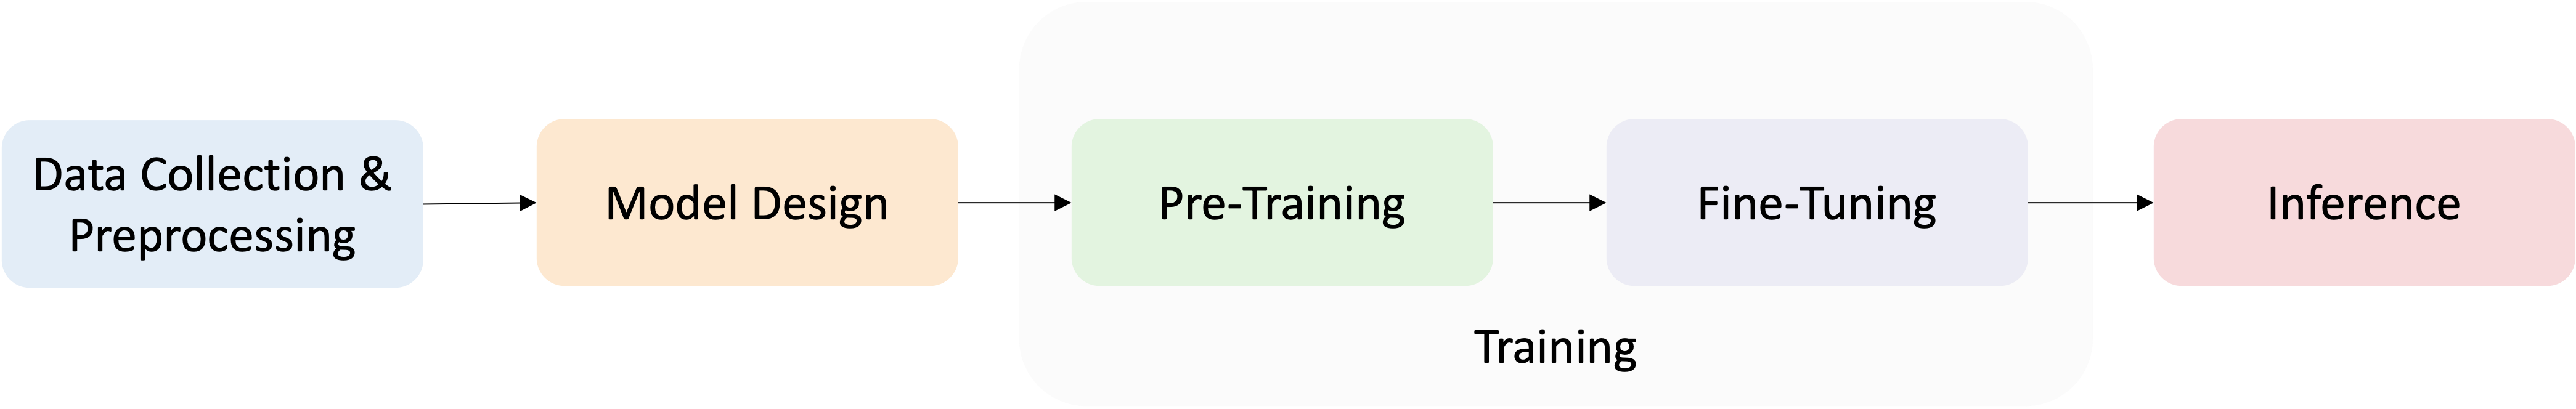
\includegraphics[width=\textwidth]{Grafiken/Efficient_Survey_Steps.png}
    \caption{Adapted Stages of Efficiency Improvement for \gls{llm} by Treviso et al. \cite{treviso_efficient_2023}}
    \label{fig:llm_taxonomy}
\end{figure}

Section \ref{subsec:llm_fine_tuning} will explore possibilities to enhance efficiency during the fine-tuning process, while Section \ref{subsec:llm_compression} will delve into the topic of model compression, which is applicable to the \textit{Inference} step in Figure \ref{fig:llm_taxonomy}.


% \begin{figure}
%     \centering
%     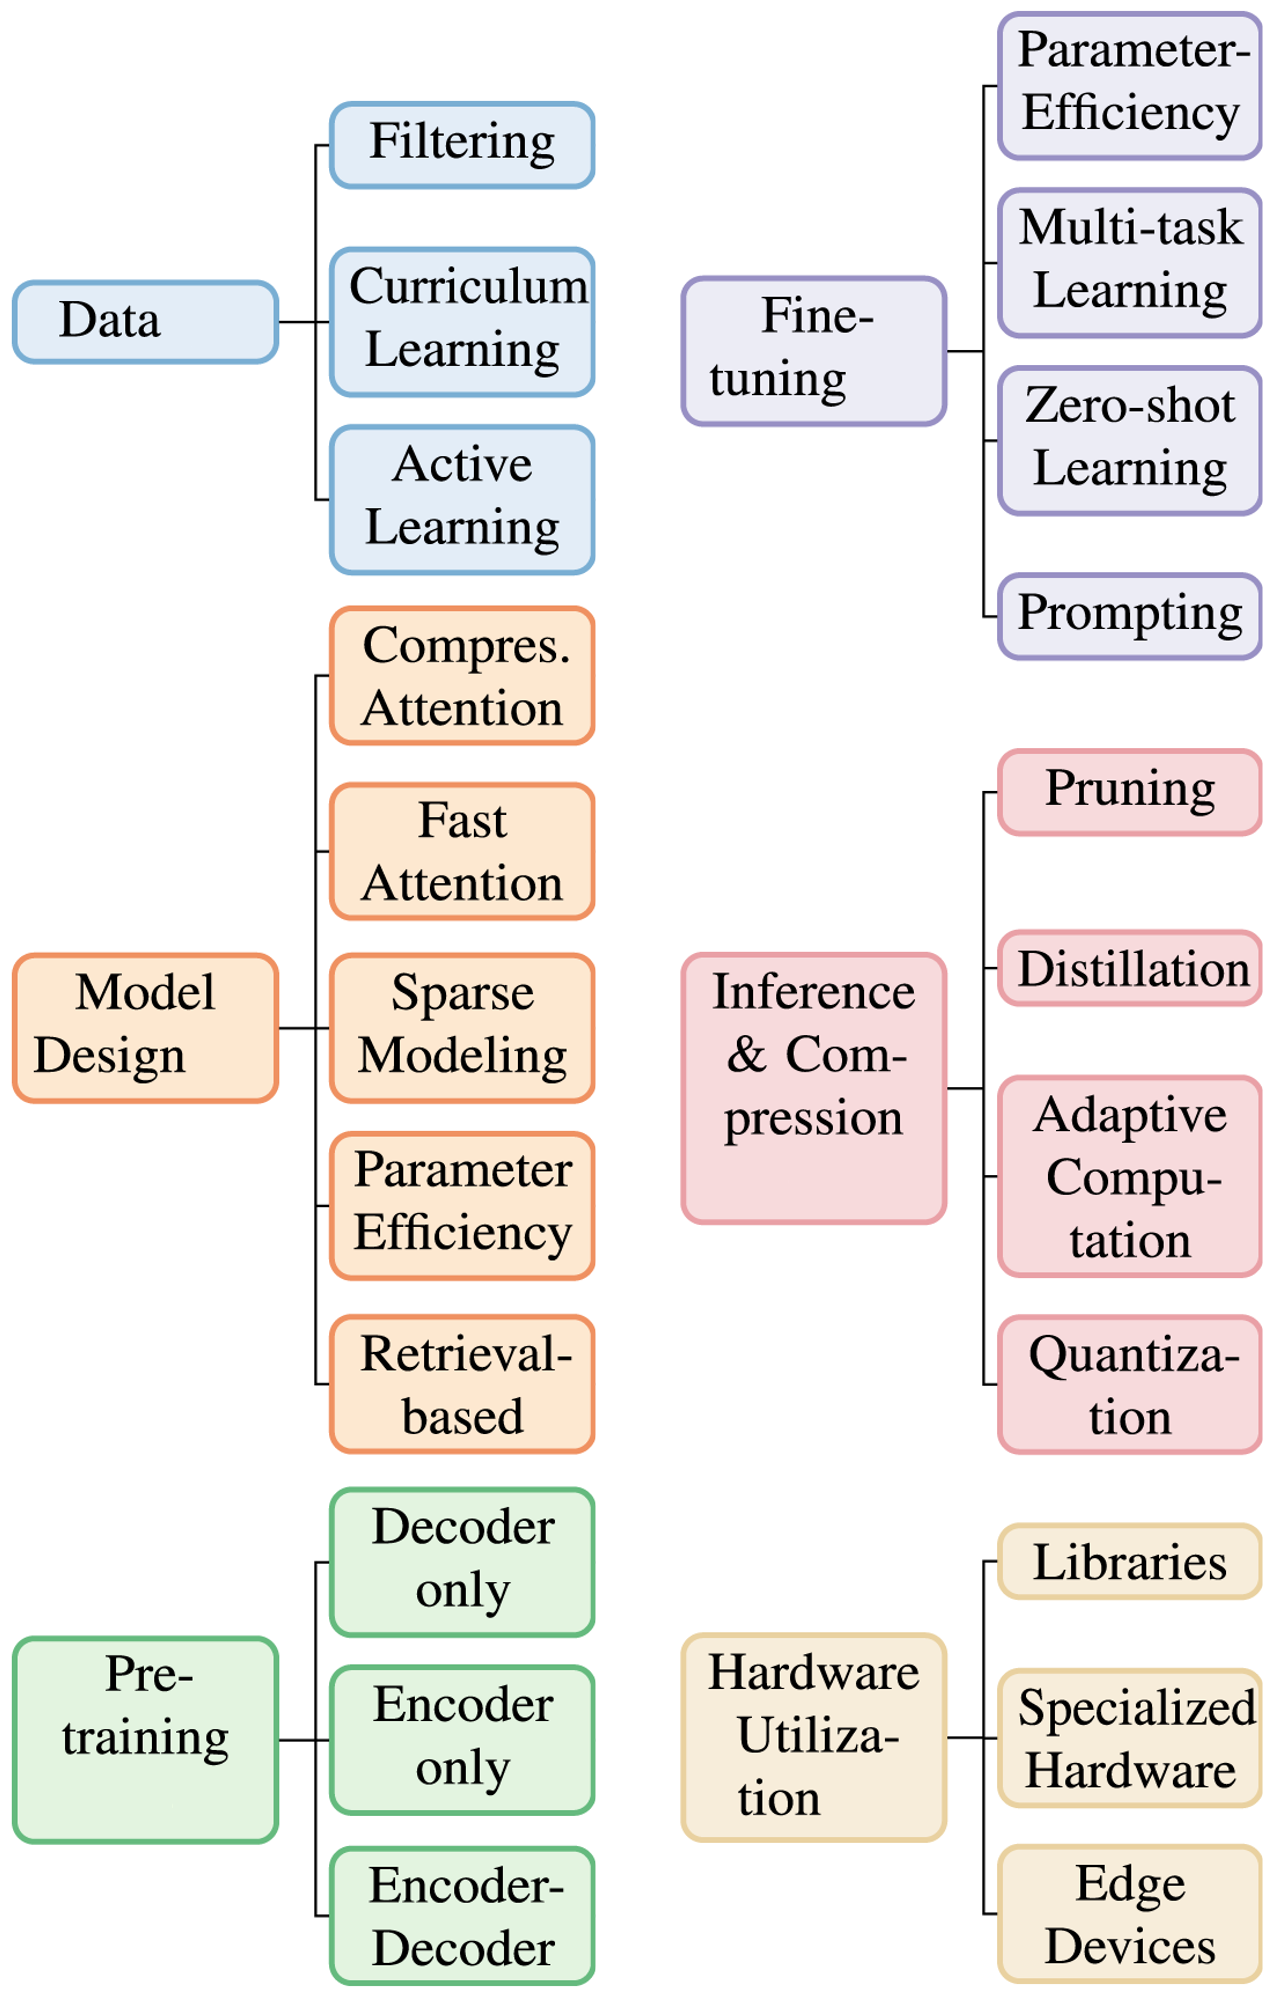
\includegraphics[width=\textwidth]{Grafiken/Efficient_Survey_Taxonomy.png}
%     \caption{Adjusted Taxonomy of efficiency improvement for \gls{llm} by Treviso et. al. \cite{treviso_efficient_2023}}
%     \label{fig:llm_taxonomy_2}
% \end{figure}

\subsection{Fine-Tuning}
\label{subsec:llm_fine_tuning}

Hu et al. \cite{hu_lora_nodate} demonstrated the significant benefits of fine-tuning GPT-3 for few-shot applications, highlighting the remarkable improvements it can achieve. This is further supported by the experiments conducted by Chung et al. \cite{chung_scaling_2022}.

Efficient fine-tuning of \gls{llm}s can be categorized into three distinct approaches: \textit{Parameter Efficiency}, \textit{Multi-task Learning}, and \textit{Prompting}. Figure \ref{fig:llm_fine_tuning} provides an overview of these approaches along with their corresponding methods.

\begin{figure}
    \centering
    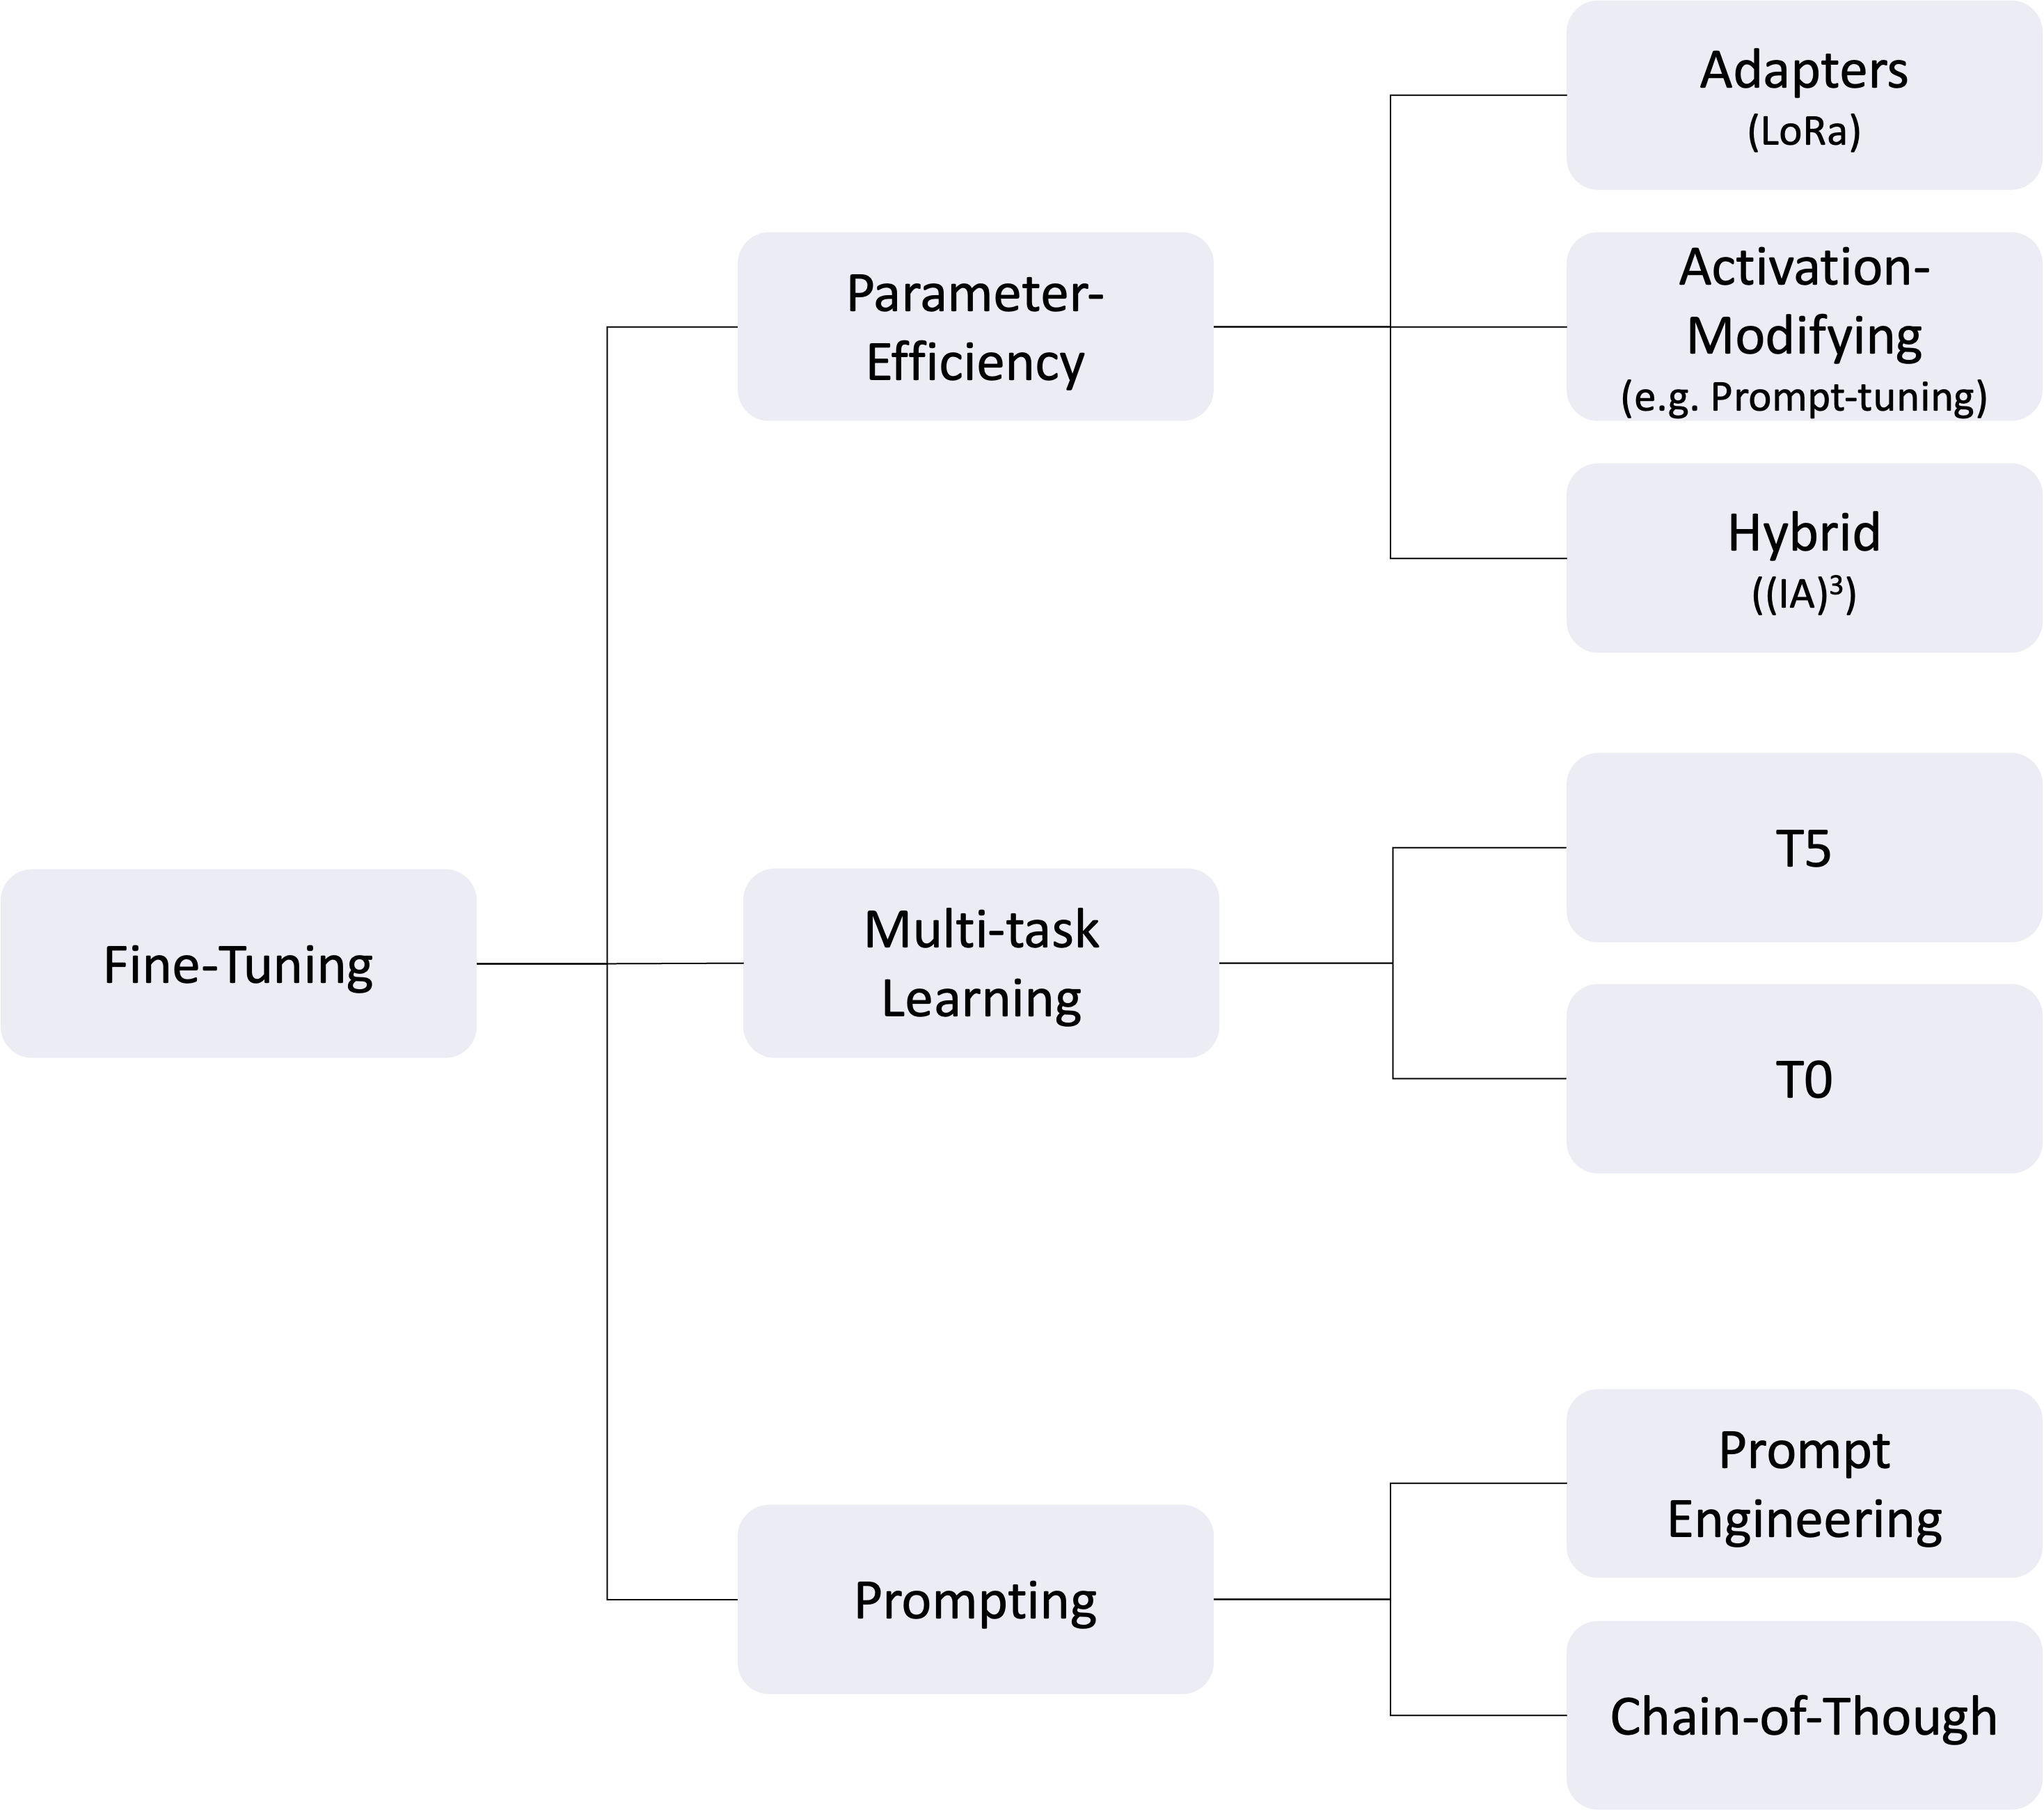
\includegraphics[width=0.8\textwidth]{Grafiken/fine_tuning_approaches.png}
    \caption{Adapted Fine-Tuning Approaches for \gls{llm} by Treviso et al. \cite{treviso_efficient_2023}}
    \label{fig:llm_fine_tuning}
\end{figure}

\textbf{Parameter Efficiency} is commonly referred to as \textbf{\gls{peft}} \cite{noauthor_peft_nodate}. A notable \gls{peft} approach is \gls{lora}, developed by Hu et al. \cite{hu_lora_nodate}. \gls{lora} falls under the category of Adapters, a term coined because it revolves around the concept of freezing the parameters of the \gls{llm} and fine-tuning only a small set of task-specific parameters, which can be swapped depending on the desired downstream task. Unlike some other Adapter-based methods \cite{houlsby_parameter-efficient_2019}, \gls{lora} does not introduce additional inference latency due to the merging of trainable matrices with frozen weights. Moreover, \gls{lora} can be seamlessly combined with many other \gls{peft} methods.

In practice, given a pre-trained weight matrix \(W_0 \in \mathbb{R}^{d \times k}\), which is typically full-rank between layers, the update can be constrained to be a low-rank composition: \(W_0 + \triangle W = W_0 + BA\), where \(B \in \mathbb{R}^{d \times r}\), \(A \in \mathbb{R}^{r \times k}\), and the rank \(r \ll \min(d, k)\). While \(W_0\) remains frozen during training, \(A\) and \(B\) become trainable parameters. The forward pass \(h = W_0x\) can be represented as the following sum:

\begin{equation}
    h = W_0x + \triangle Wx = W_0x + BAx
\end{equation}

Figure \ref{fig:lora} illustrates the architecture and initialization during training. The parameters of \(A\) are randomly sampled using Gaussian initialization, while \(B\) is initialized to 0.

Other \gls{peft} techniques include \textbf{prompt-tuning} \cite{lester_power_2021} and \textbf{prefix-tuning} \cite{li_prefix-tuning_2021}. Both approaches are similar in the way they leverage task-specific modifications to the input to guide the model's behavior. They involve concatenating learned vectors to activations or embedding sequences, making them activation-modifying \gls{peft} methods.

A \gls{peft} approach that can be considered a hybrid between \gls{lora} and activation-modifying techniques is \textbf{$\text{(IA)}^3$} \cite{liu_few-shot_2022}. What sets $\text{(IA)}^3$ apart is its focus on \gls{llm}s designed explicitly for multi-task learning, as all existing \gls{peft} techniques significantly underperformed in experiments conducted by Liu et al. \cite{liu_few-shot_2022}. In $\text{(IA)}^3$, the model's activations are rescaled using element-wise multiplication with learned vectors, known as adaptors. Specifically, $\text{(IA)}^3$ employs three learned vectors: \(l_k \in \mathbb{R}^{d_k}\) for keys and \(l_v \in \mathbb{R}^{d_v}\) for values in self-attention and encoder-decoder attention mechanisms, as well as \(l_{ff} \in \mathbb{R}^{d_{ff}}\) for the feed-forward network. The rescaling is incorporated into the attention mechanism as follows:

\begin{equation}
    \operatorname{softmax}\left(\frac{Q\left(l_{k} \odot K^T\right)}{\sqrt{d_k}}\right)\left(l_{v} \odot V\right)
\end{equation}

For the feed-forward network, the rescaling is implemented as follows, where \(\gamma\) represents the feed-forward activation:

\begin{equation}
    (l_{ff} \odot \gamma (W_1x))W_2
\end{equation}

In summary, \textbf{$\text{(IA)}^3$} is a \gls{peft} approach specifically designed for multi-task learning, and it appears to outperform \gls{lora} in terms of the number of parameters added and training computation costs.

\textbf{Multi-task Learning} refers to the concept of fine-tuning a \gls{prlm} on various tasks to achieve better zero-shot and fine-tuning performance. One of the most prominent \gls{prlm}s trained on multiple NLP tasks is T5 \cite{raffel_exploring_2023}. Liu et al. \cite{liu_few-shot_2022} demonstrated that a generically trained T5 model can be few-shot fine-tuned with approximately 10\% of the parameters of \gls{lora}, at a lower computational cost, while achieving higher accuracy in classification tasks\footnote{Currently, there is no experiment comparing LoRa and $\text{(IA)}^3$ on QA tasks}. This is made possible, due to using $\text{(IA)}^3$ as \gls{peft}.

\textbf{Prompting} refers to the general concept of presenting a task as a textual instruction to a \gls{llm} \cite{brown_language_2020}. Recent advances have even led to the development of a new sub-task and job role called \textit{Prompt Engineering} \cite{white_prompt_2023}. It's worth noting that different prompts with the same intent can yield different results, making the selection of the right prompt a challenge in itself \cite{liu_gpt_2021}. Furthermore, concepts like \gls{cot} prompts have been developed. In \gls{cot} prompts, the given example in a Few-shot prompt is redesigned to mimic step-by-step reasoning and conclusions known from the way humans think, aiming to achieve higher performance in Zero- and Few-shot scenarios simply by adjusting the explicit natural language prompt \cite{wei_chain--thought_2023}.

\begin{figure}
    \centering
    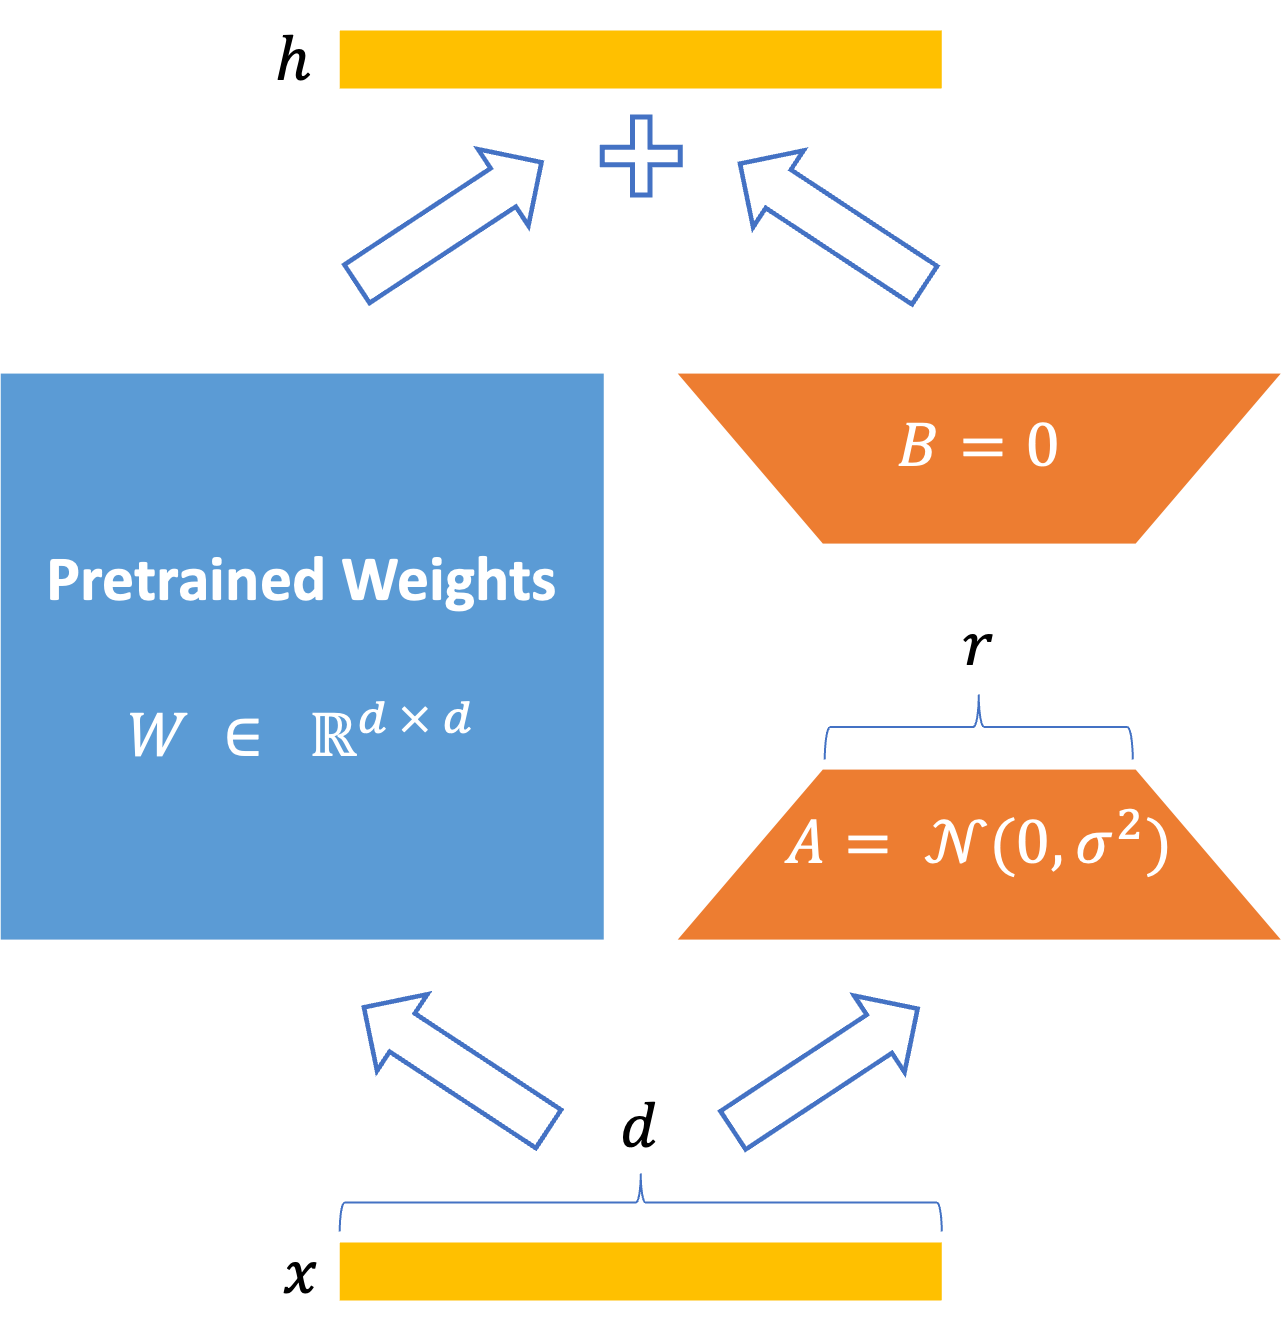
\includegraphics[width=0.5\textwidth]{Grafiken/Lora.png}
    \caption{\gls{lora} by Hu et. al. \cite{hu_lora_nodate}}
    \label{fig:lora}
\end{figure}


\subsection{Compression}
\label{subsec:llm_compression}

\section{Related Work}
\label{sec:related_work}

\subsection{Question Answering based on PDFs}
\label{subsec:related_work_dbqa}

\textbf{PDF Question Answering} is the task of providing answers to questions related to the content of one or multiple documents \cite{mathew_document_2021}. The field of research which actively explores this the closest is Visual Document Question Answering. It works on the development of an IR-QA system that operates on images of documents. An exemplary architecture and a general pipeline for transforming PDFs into an IR-QA system is presented by McDonald et al. \cite{mcdonald_detect_2022}. They developed their zero-shot framework around the QASPER dataset but used the original PDFs instead of extracted text via LaTeX. Moreover, readily available open-source tools like V-Doc \cite{ding_v-doc_2022} simplify the deployment and testing of datasets, models, and IR-QA systems of the Visual Document Question Answering domain.

More recently, the open-source framework \textit{Langchain} has gained tremendous attention\footnote{As of September 24, 2023, Langchain has received 63k stars on GitHub}. Langchain focuses on harnessing LLMs using chains, which are essentially prompts for an LLM that can be chained together \cite{noauthor_langchain-ailangchain_nodate}. They also provide documentation on building a QA system based on PDFs \cite{noauthor_question_nodate}. Similarly, \textit{OpenAI} offers a Retrieval Plugin for \textit{ChatGPT} \cite{noauthor_chatgpt_2023}, also an open-source repository. These QA systems adhere to the paradigms established in previous works such as \cite{karpukhin_dense_2020,ni_large_2021,neelakantan_text_2022,lewis_retrieval-augmented_2021}. Specifically, this entails:

\begin{itemize}
    \item Given a text corpus, documents can be retrieved by extracting relevant passages. Data cleaning of the corpus is optional but not necessary. Therefore, these systems employ a \textit{direct extraction} approach, especially when dealing with PDFs.
    \item Utilizing large-scale, diversely trained encoders. Representation-based Retrievers, when equipped with sufficient trainable parameters and diverse training datasets, often yield comparable results to fine-tuned, more complex retrieval models \cite{ni_large_2021,neelakantan_text_2022}.
    \item Using the LLM as a generative reader for QA, as demonstrated in the work of Izacard et al. \cite{izacard_leveraging_2021}.
\end{itemize}

Non-LLM research for \gls{qa} based on PDFs is notably scarce. In the field of ODQA, discussions regarding applicable frameworks that encompass the entire pipeline from PDFs to \gls{qa} are infrequent. Instead, the focus often revolves around constructing \gls{qa} systems using predefined and well-supervised datasets. However, there is some research that explores the feasibility of deploying high-performing \gls{qa} systems in out-of-domain scenarios, bypassing the initial stage of data preprocessing (from PDFs to passages). This research strives to outline possibilities for using a \gls{qa} system in real-world passage collections.

\noindent \textbf{Applying Dense Retrievers Out-of-Domain}: As emphasized by Thakur et al. in their \enquote{Heterogeneous Benchmark for Zero-shot Evaluation of Information Retrieval Models} (BEIR) \cite{thakur_beir_2021}, dense retrievers exhibit weak out-of-domain performance. Lyu et al. \cite{farea_evaluation_2022} also demonstrate the limited generality of dense retrievers when trained in one subdomain and subsequently applied in a different one. This underscores the conclusion that there are two approaches to employing retrievers in out-of-domain scenarios: (1) fine-tuning or (2) zero-shot, but with large encoders that have been trained on diverse datasets \cite{ni_large_2021}.

The challenge with fine-tuning lies in the unavailability of labeled data, which is typically required for supervised models in the form of tuples such as $(question, answer, context)$. Several diverse approaches have been developed to address this issue. One approach employs \gls{qg} techniques, as exemplified by Promptagator \cite{dai_promptagator_2022}, which utilizes LLMs. Another strategy involves the use of Mixture-of-Experts and meta-learning algorithms \cite{chen_improving_2021}. Some researchers have explored semi-supervised training datasets, as demonstrated by Sachan et al. \cite{sachan_questions_2023}, who developed ART, a training framework for dense retrievers that only requires questions and surpasses the standard \gls{dpr} training implementation. At the current point in time there is no state-of-the-art appraoch to fine-tune a dense retriever on a small subdomain dataset.

In their study, Reddy et al. \cite{reddy_synthetic_2022} addressed the challenge of creating a \gls{qa}-System for Covid-19-related documents, where no supervised \gls{qa} dataset was available. Consequently, they conducted a comparison between the performance of zero-shot BM25 and \gls{dpr}. Their findings revealed that BM25 outperformed \gls{dpr} on the BiosQA \gls{qa} dataset, closely related to the Covid-19 domain. Throughout their experiments, they evaluated various approaches, including simple zero-shot techniques, fine-tuning of \gls{dpr} using \gls{qg} via BART, which yielded superior results. Notably, the most effective retriever for unsupervised domain adaptation was a combination of BM25 and unsupervised fine-tuned \gls{dpr}.

Furthermore, Gururangan et al. \cite{gururangan_dont_2020} demonstrated in their experiments that fine-tuning \glspl{prlm} on domain-specific language or, even better, task-specific data led to a significant performance boost.

Gholami et al. \cite{gholami_zero-shot_2021} experimented with non-fine-tuned dense retrievers on a non-\gls{qa} dataset, specifically a collection of AWS documentations. Their results, particularly for the retrieval component, were sobering, aligning with the findings of benchmark studies by Thakur et al. \cite{thakur_beir_2021} and Lyu et al. \cite{farea_evaluation_2022}.

On the other hand, there exist reader components with a high degree of generalizability, as demonstrated by UnifiedQA-v2 \cite{khashabi_unifiedqa-v2_2022}, an extractive reader, and T5 \cite{raffel_exploring_2023}, a generative reader. So the main challenge, when building a \gls{ir}-\gls{qa}-System, lays within the implementation and adaptation of the retriever component.


\subsection{Open-domain Conversational Question Answering ???} 
\label{subsec:related_work_cqa}

\textbf{From single-turn Question Answering to Conversation}

\textbf{Synthetic Datageneration}



%%%%%%%%%%%%%%%%%%%%%%%%%%%%%%%%%%%%%%%%%%%%%%%%%%%%%%%%%%%%
\newpage
%%%%%%%%%%%%%%%%%%%%%%%%%%%%%%%%%%%%%%%%%%%%%%%%%%%%%%%%%%%%

\chapter{Open-domain QA Chatbot over PDFs}
\label{chap:main}

This chapter outlines the methods and techniques employed in the development of a conversational question-answering system designed for PDFs. The chapter is structured as follows: Section \ref{sec:overview} provides an overview of the desired use case, its objectives, and constraints concerning a Conversational Question Answering System. Section \ref{sec:conrag} presents a general framework that can be utilized as a decision tree for the practical implementation of a Conversational Question Answering System for PDFs. Its subsections will highlight and discuss the components introduced within the framework.

\section{Overview and Objective}
\label{sec:overview}

The primary use case addressed in this thesis can be summarized as follows: Imagine having a collection of PDF files, and our goal is to create a chatbot capable of engaging in conversations about the knowledge within these PDFs. This chatbot should provide accurate answers to questions based on the content of the PDFs and furnish supporting evidence from these documents. Furthermore, it should enable users to have a conversational query experience, allowing them to ask follow-up questions and engage in dialogue with the chatbot based on its previous responses. Figure \ref{fig:use-case} illustrates an example of this use case.

\begin{figure}
    \centering
    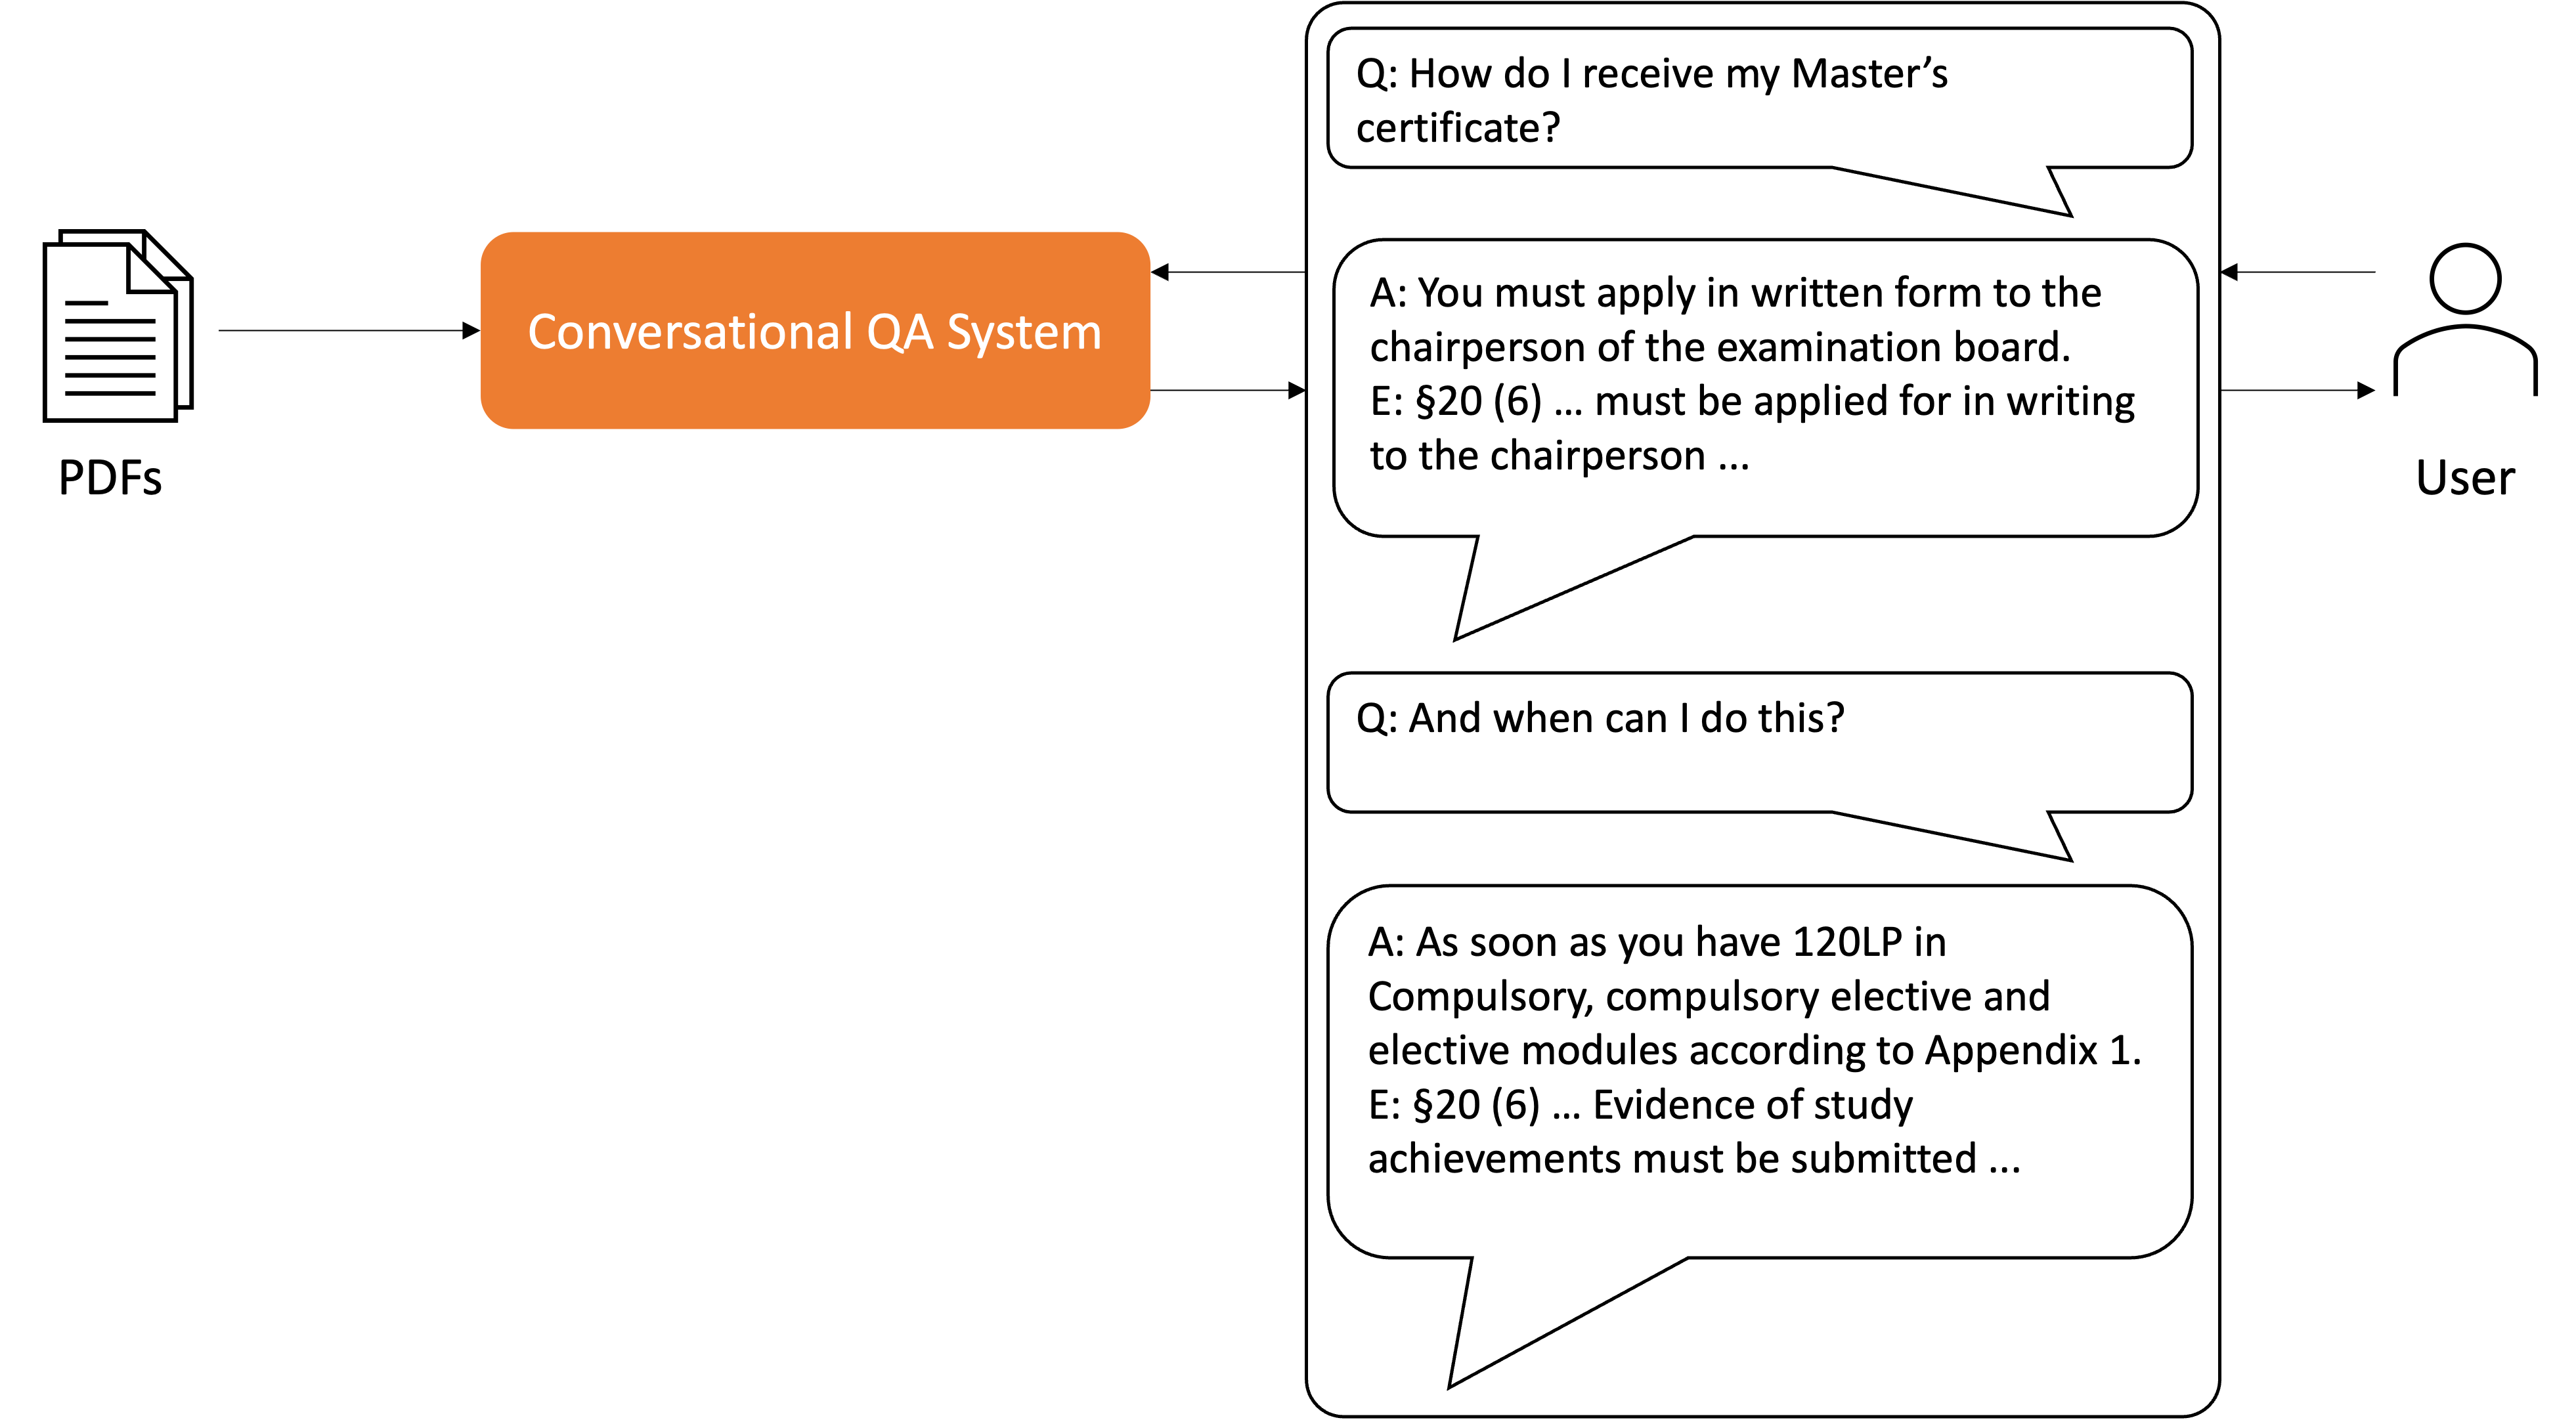
\includegraphics[width=0.8\textwidth]{Grafiken/Use_Case.png}
    \caption{Overview of the Example Use-Case}
    \label{fig:use-case}
\end{figure}

Currently, to the best of my knowledge, there is no scientific paper or similar resource offering a comprehensive framework or pipeline to address this use case. This thesis aims to bridge this gap by presenting a framework and pipeline designed to tackle this specific scenario. Figure \ref{fig:overview-system-architecture} provides an overview of the system architecture. The system follows the \gls{rag} architecture, as detailed in Section \ref{subsec:qa_retrieval}, which extends the classical Retriever-Reader with a \gls{llm} as a Reader, capable of incorporating parametric knowledge. To extend \gls{rag} to a \gls{convqa}, a \gls{cqu} unit, as introduced in Section \ref{subsec:cqa_contextual_query_understanding}, is essential. This novel architecture will be termed \textbf{\gls{conrag}}. The extraction pipeline will be discussed in Section \ref{subsec:extract}, with its primary tasks being the extraction of passages from the provided set of PDFs, the creation of an index, and the optional generation of synthetic training data. The three major modules comprising the architecture, namely the \textit{Retriever}, \textit{Reader}, and \textit{\gls{cqu}}, will be elaborated in their respective sections: \ref{subsec:retriever}, \ref{subsec:reader}, and \ref{subsec:cqu}.

\begin{figure}
    \centering
    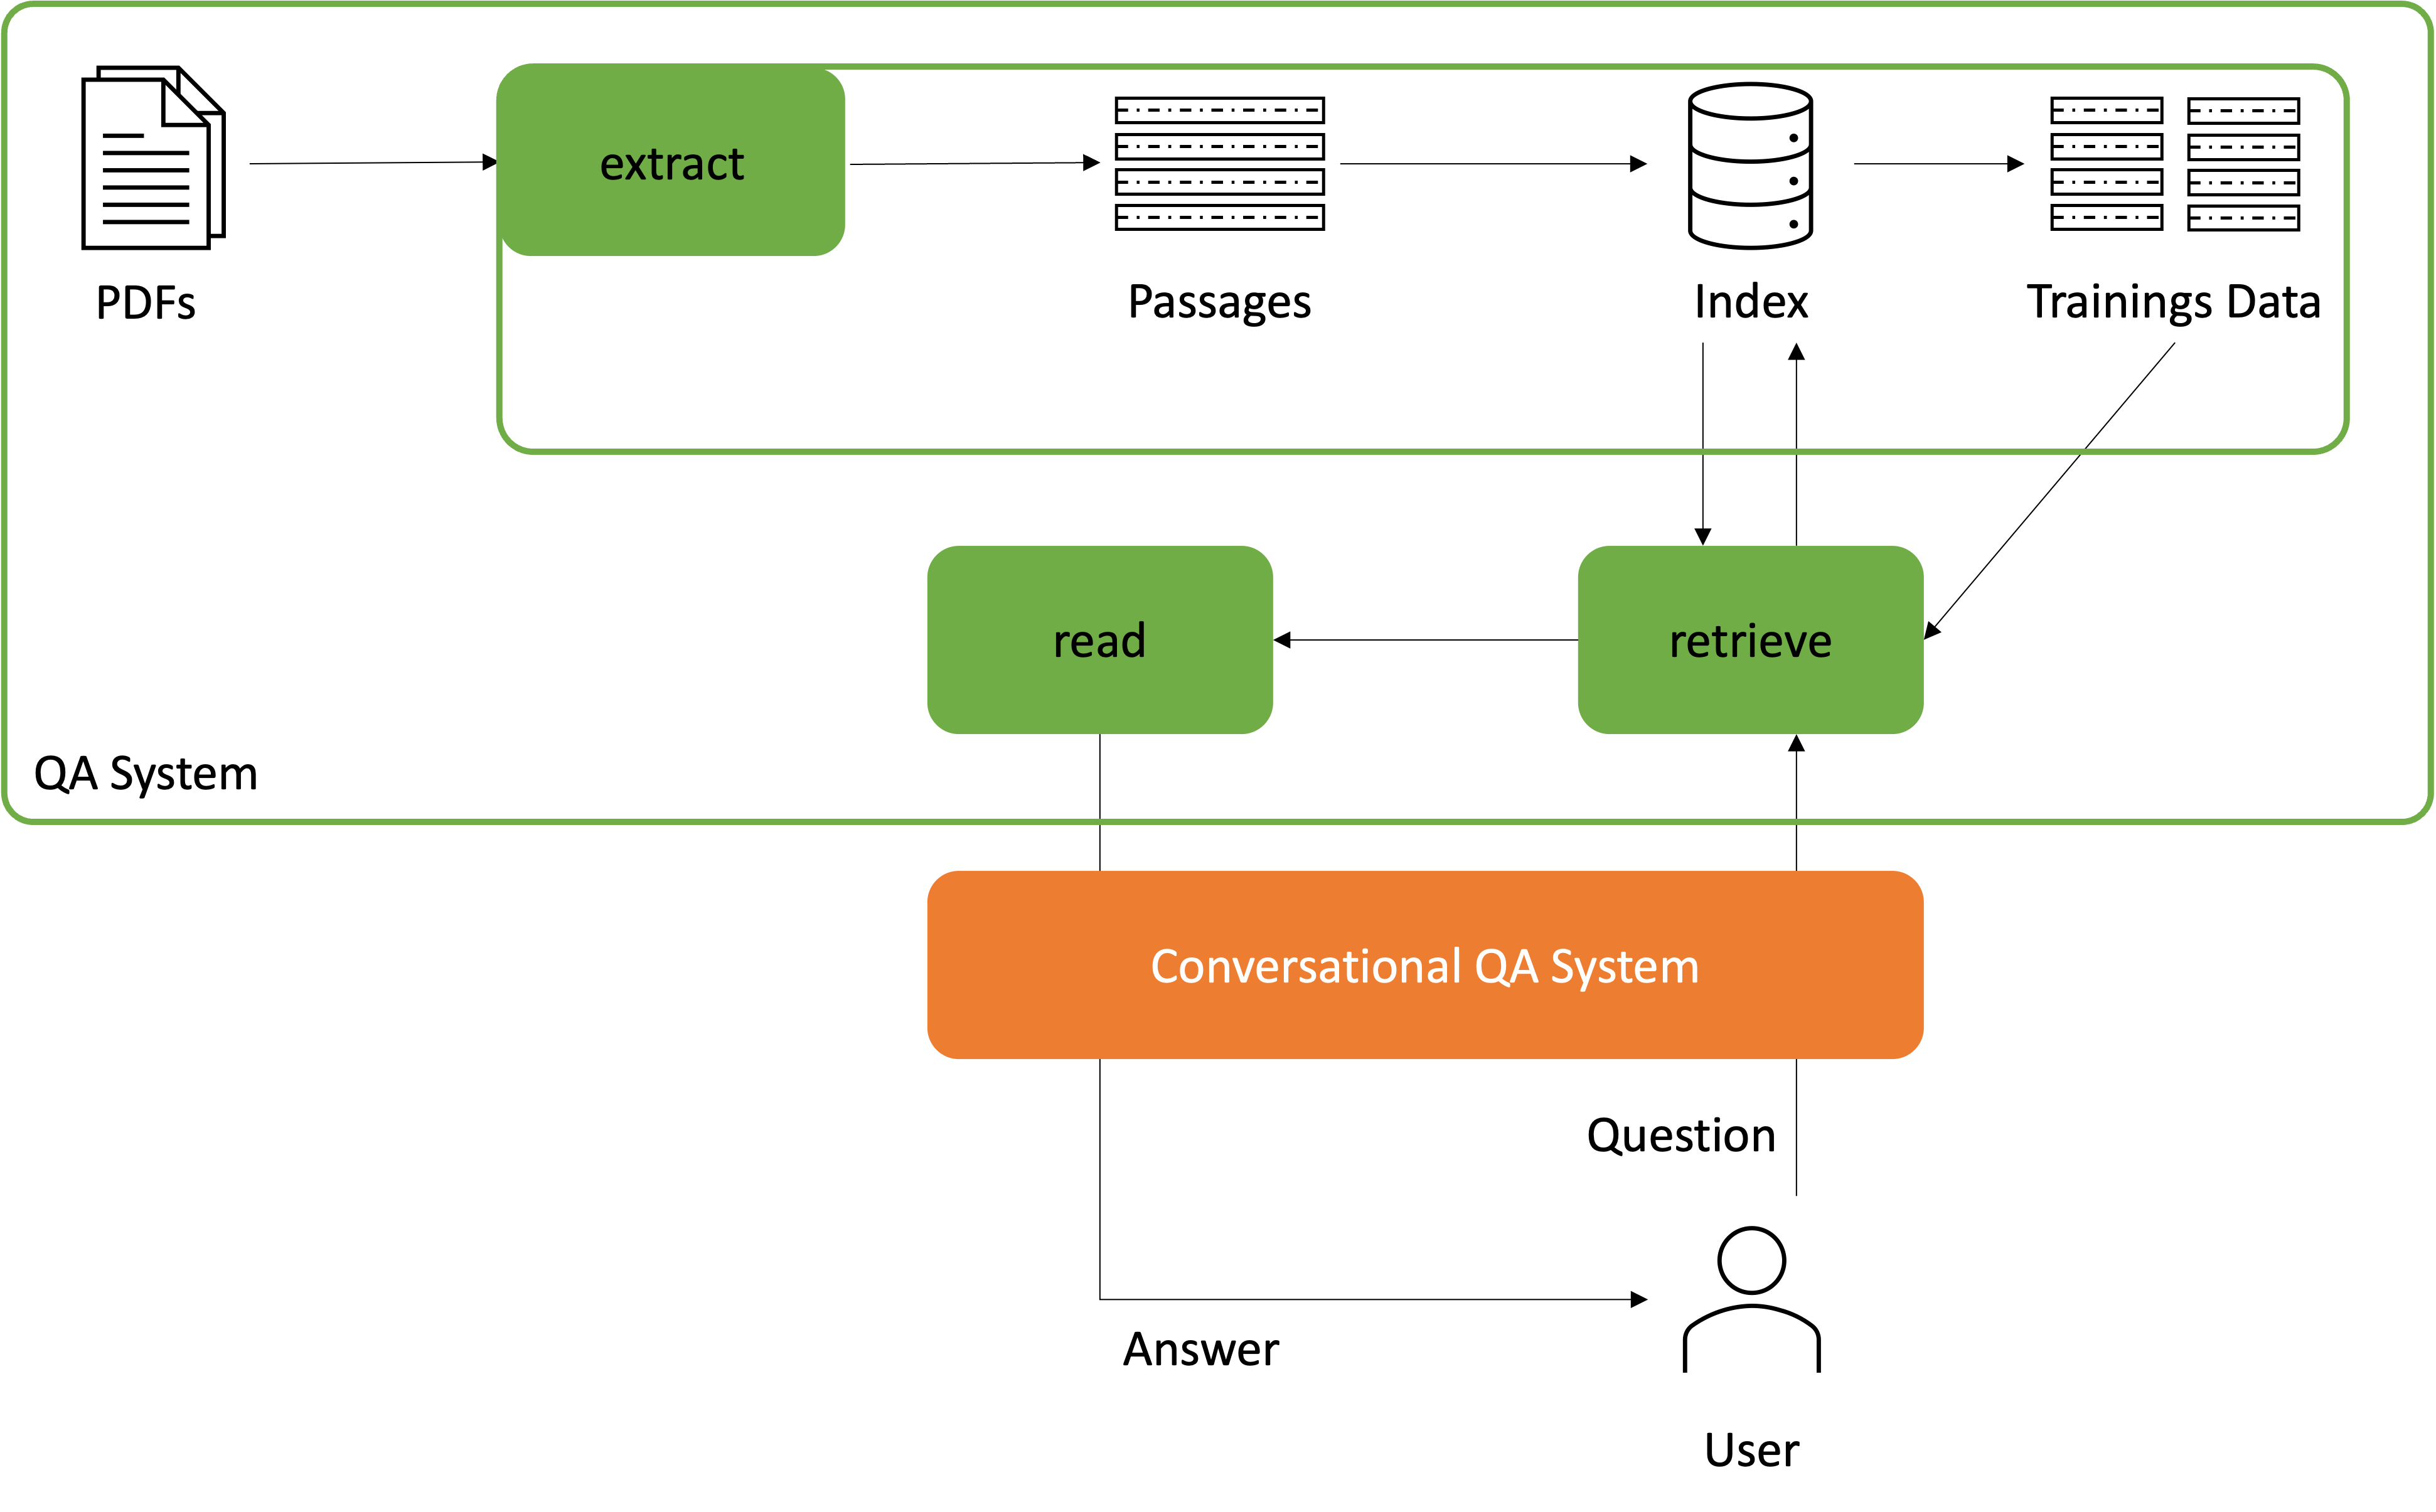
\includegraphics[width=0.8\textwidth]{Grafiken/System_Architecture.png}
    \caption{Overview of the System Architecture}
    \label{fig:overview-system-architecture}
\end{figure}

To summarize, the objectives of the QA capabilities of the system are as follows:

\begin{enumerate}
    \item Utilize \textbf{PDFs} as the primary \textbf{knowledge source}.
    \item Enable the QA-System to handle a \textbf{variety of question types}, including: \textbf{extractive}, \textbf{abstractive}, and \textbf{boolean questions}.
    \item \textbf{Provide references} to PDF snippets \textbf{as evidence to answers}.
    \item Ensure the pipeline's generalizability, allowing it to adapt to new domains or knowledge sources with \textbf{minimal or no supervision} and \textbf{small datasets}.
    \item Design the pipeline to be \textbf{feasible without the need for datacenter-grade hardware resources}, making it accessible for development on standard research hardware.
    \item \textbf{Prioritize accuracy as the primary objective}, as constraining memory consumption is indirectly covered in point (5). \textbf{Latency is not a primary concern}, as the system is not intended for real-time use and will not be optimized for that.
\end{enumerate}


Regarding the ConvQA-System, the objectives are as follows:

\begin{enumerate}
    \item Enable the ConvQA-System to \textbf{handle} the following follow-up \textbf{question types: drilling-down, clarification, topic shift} and \textbf{comparison}.
    \item Be able to take Initiative in the form of \textbf{clarifying questions}.
    \item The \textbf{memory} will be \textbf{limited to a session}.
\end{enumerate}

\section{Problem Statement}
\label{sec:problem_statement}

The following Section will layout the problem of document-based \gls{convqa}. 

Substantially the fundamental thing given, is some sort of \textit{Document}. A \textit{Document} can be any type of structured or unstructured file, which is being used for storing and displaying information. Examples could be HTML (structured) or PDF (unstructured) files. A \textit{Document} consits of content $C_d$, a collection of strings $c_d$, whereas the content $C_d$ has to have at least one $c_d$, but can contain also multiple, a topic $t$, which is an abstract entity and has no finite set of $T$, a topic could be for example \enquote{Examination Regulation of the Master of Data and Computer Science at the University Heidelberg}, and a unique identifier $UID_d$, therefore a \textit{Document} $d = (C_d,t, UID_d)$. For this thesis we will only cosider textual content $C_d$ and not figures or images. Out of the necessity, for knowledge granularity and precise information context, we will define \textit{Passages} next. A \textit{Passage} $p$ is a subset of a textual content strings $c_d \in C_d$. The granularity of $p$ can be defined use-case specific. If $p$ is a sentence, 100 tokens or other depends on the given scenario. Nevertheless, every $p$ contains a reference to the orgianl document $d$ it was taken from and has it's own unique identifier $UID_p$. This leads to the following \textit{Passage Model}:
\begin{definition}
    \textbf{(Passage Model)} A passage $p$ is a subset of a textual content string $c_d \in C_d$ of a document $d = (C_d,t, UID_d)$, whereas $p = (content, UID_p, UID_d)$.
    \label{def:passage_model}
\end{definition}

For the ease of notation, we will refer to the content of a passage $p$ as $p$ itself in the following. The collection of all \textit{Passages} $P$ will be refered to as the \textit{Knowledge Source}. 

Next we need to define what a \textit{Question} is. For this problem, a question consits of a string - $content$, which incorporates a question in natural language and an intent $i \in I$, which also again is an abstract entity, refereing to the actual information need $q$ should fullfill. The \textit{Question Model} can therefore be defined as follows:

\begin{definition}
    \textbf{(Question Model)} A question $q$ is a tuple $(content, i)$, whereas $content$ is a string and $i \in I$.
    \label{def:question_model}
\end{definition}

Also here we will refer to the content of a question $q$ as $q$ itself in the following, for reducing the complexity of the notation.

Naturally given a \textit{Question}, there has to be an \textit{Answer}. An \textit{Answer} $a$ is a string, which is the answer to a \textit{Question} $q$, given that it fullfills the intent $i$ of $q$. This is being refered to as $I(q,a) = 1$. Formally we define an \textit{Answer} as:

\begin{definition}
    \textbf{(Answer Model)} An answer $a$ is a string, which answers a given question $q$ under the condition, that the search intent of $q$ is satisfied $I(q,a) = 1$.
    \label{def:answer_model}
\end{definition}

In terms of conversations, we split an exchange between two agents into \textit{Turns} as described in Section \ref{subsec:cqa_basics}. Generally speaking, a \textit{Turn} $h$ consists of a tuple $(q,a)$, whereas the $a$ is the response to $q$. \textit{Turns} happen in order and have a relation between each other. Therefore we refer to the collection of multiple \textit{Turns} within one conversation as \textit{History} $H$.

\begin{definition}
    \textbf{(History Model)} A history $H$ is a collection of turns $h$, whereas $h = (q,a)$.
    \label{def:history_model}
\end{definition}

As we now have elaborated, what \textit{Questions}, \textit{Knowledge Source}, \textit{Answers} and \textit{History} are, we're ready to define the problem of \gls{convqa}:

\begin{definition}
    \textbf{(Conversational Question Answering Task)} Given a new question $q_{i+1}$ and a history $H$ with $i$-many turns $h$, a model ($M$) should generate an answer $a_{i+1}$, based on the provided knowledge in the knowledge source $P$, which satisfies the search intent $i$ of $q_{i+1}$. Next to the answer $a_{i+1}$, $M$ should return $p$ as evidence from $P$. Formally:
    \begin{align*}
        \mathbf{M: (q_{i+1}, H, P) \rightarrow (a_{i+1}, p)}
    \end{align*}
    \label{def:task}
\end{definition}

\section{Conversational Retrieval-Augmented Generation}
\label{sec:conrag}

In order to provide a solution to the Task of \gls{convqa} as defined in Definition \ref{def:convqa}, the system must be able to perform evidence selection based on a \textit{Knowledge Source} which is an important criterion also layed out in Section \ref{sec:overview}. 

In order to now create a system architecture, which fullfills the task of model $M$ (see Definition \ref{def:task}), we will split the main task of \gls{convqa} into multiple subtasks:

\begin{enumerate}
    \item \textbf{Information Extraction:} Given a set of documents $D$, extract the textual content $C_d$ of each document $d \in D$ and create a knowledge source $P$ based on $C_d$ of every document $d \in D$.
    \item \textbf{Contextual Question Understanding:} Given a history $H$ and a new question $q_{i+1}$, generate a contextualized question $q_c$ based on $H$, sothat $I(q_c,q_{i+1}) = 1$.
    \item \textbf{Passage Retrieval:} Given a contextualized question $q_c$ and a knowledge source $P$, retrieve the $k$-most relevant passages $p$ from $P$ and combine them in an evidence set $E$.
    \item \textbf{Response Generation:} Given a contextualized question $q_c$ and a set of passages $E$, generate an answer $a$ to $q_c$ based on $E$, so that $I(q_{i+1},a) = 1$.
\end{enumerate}

There may exist other approaches to break down the task of $M$ into sub-tasks, but for this thesis, we will focus on a solution based on the four sub-tasks outlined above. The reason is simply the existing state-of-the-art research in every field of this sub-tasks, especially when it comes to the adoption of new domains. It is to be highlighed, that breaking the task of $M$ implies also an order in which the sub-tasks have to be performed. Sub-task (1) will be performed once, while (2-4) will be repeated on every new question $q_{i+1}$.

In order to develop a system which can be applied to this abstract task, we match every task with a component. The \textit{Information Extraction} sub-task will be solved by the \textit{extract} component, further detailed in Section \ref{subsec:extract}. \textit{Passage Retrieval} will be covered by the \textit{Retriever} component, further discribed in Section \ref{subsec:retriever}. The \textit{Response Generation} will be handled by the \textit{Reader} component, more precisely in this thesis we will focus on \gls{llm}s with intrinsic parametric knowledge as \textit{Reader}. This will lead to a \gls{rag} system consisting of the \textit{Retriever} and \textit{Reader}. This choice has been made due to the fact, that the latest reasearch breakthroughs sparked the interest in \gls{rag} systems in compraison towards classical Retriever-Reader systems (check herefore the related work Section \ref{sec:related_work}). Details on the \textit{Reader} component will be layed out in Section \ref{subsec:reader}. In order to now handle conversations, a \gls{cqu} unit as described in Section \ref{subsec:cqa_contextual_query_understanding} is necessary to handle the sub-task of \textit{Contextual Question Understanding}. Section \ref{subsec:cqu} will dive into the details.

\begin{figure}
    \centering
    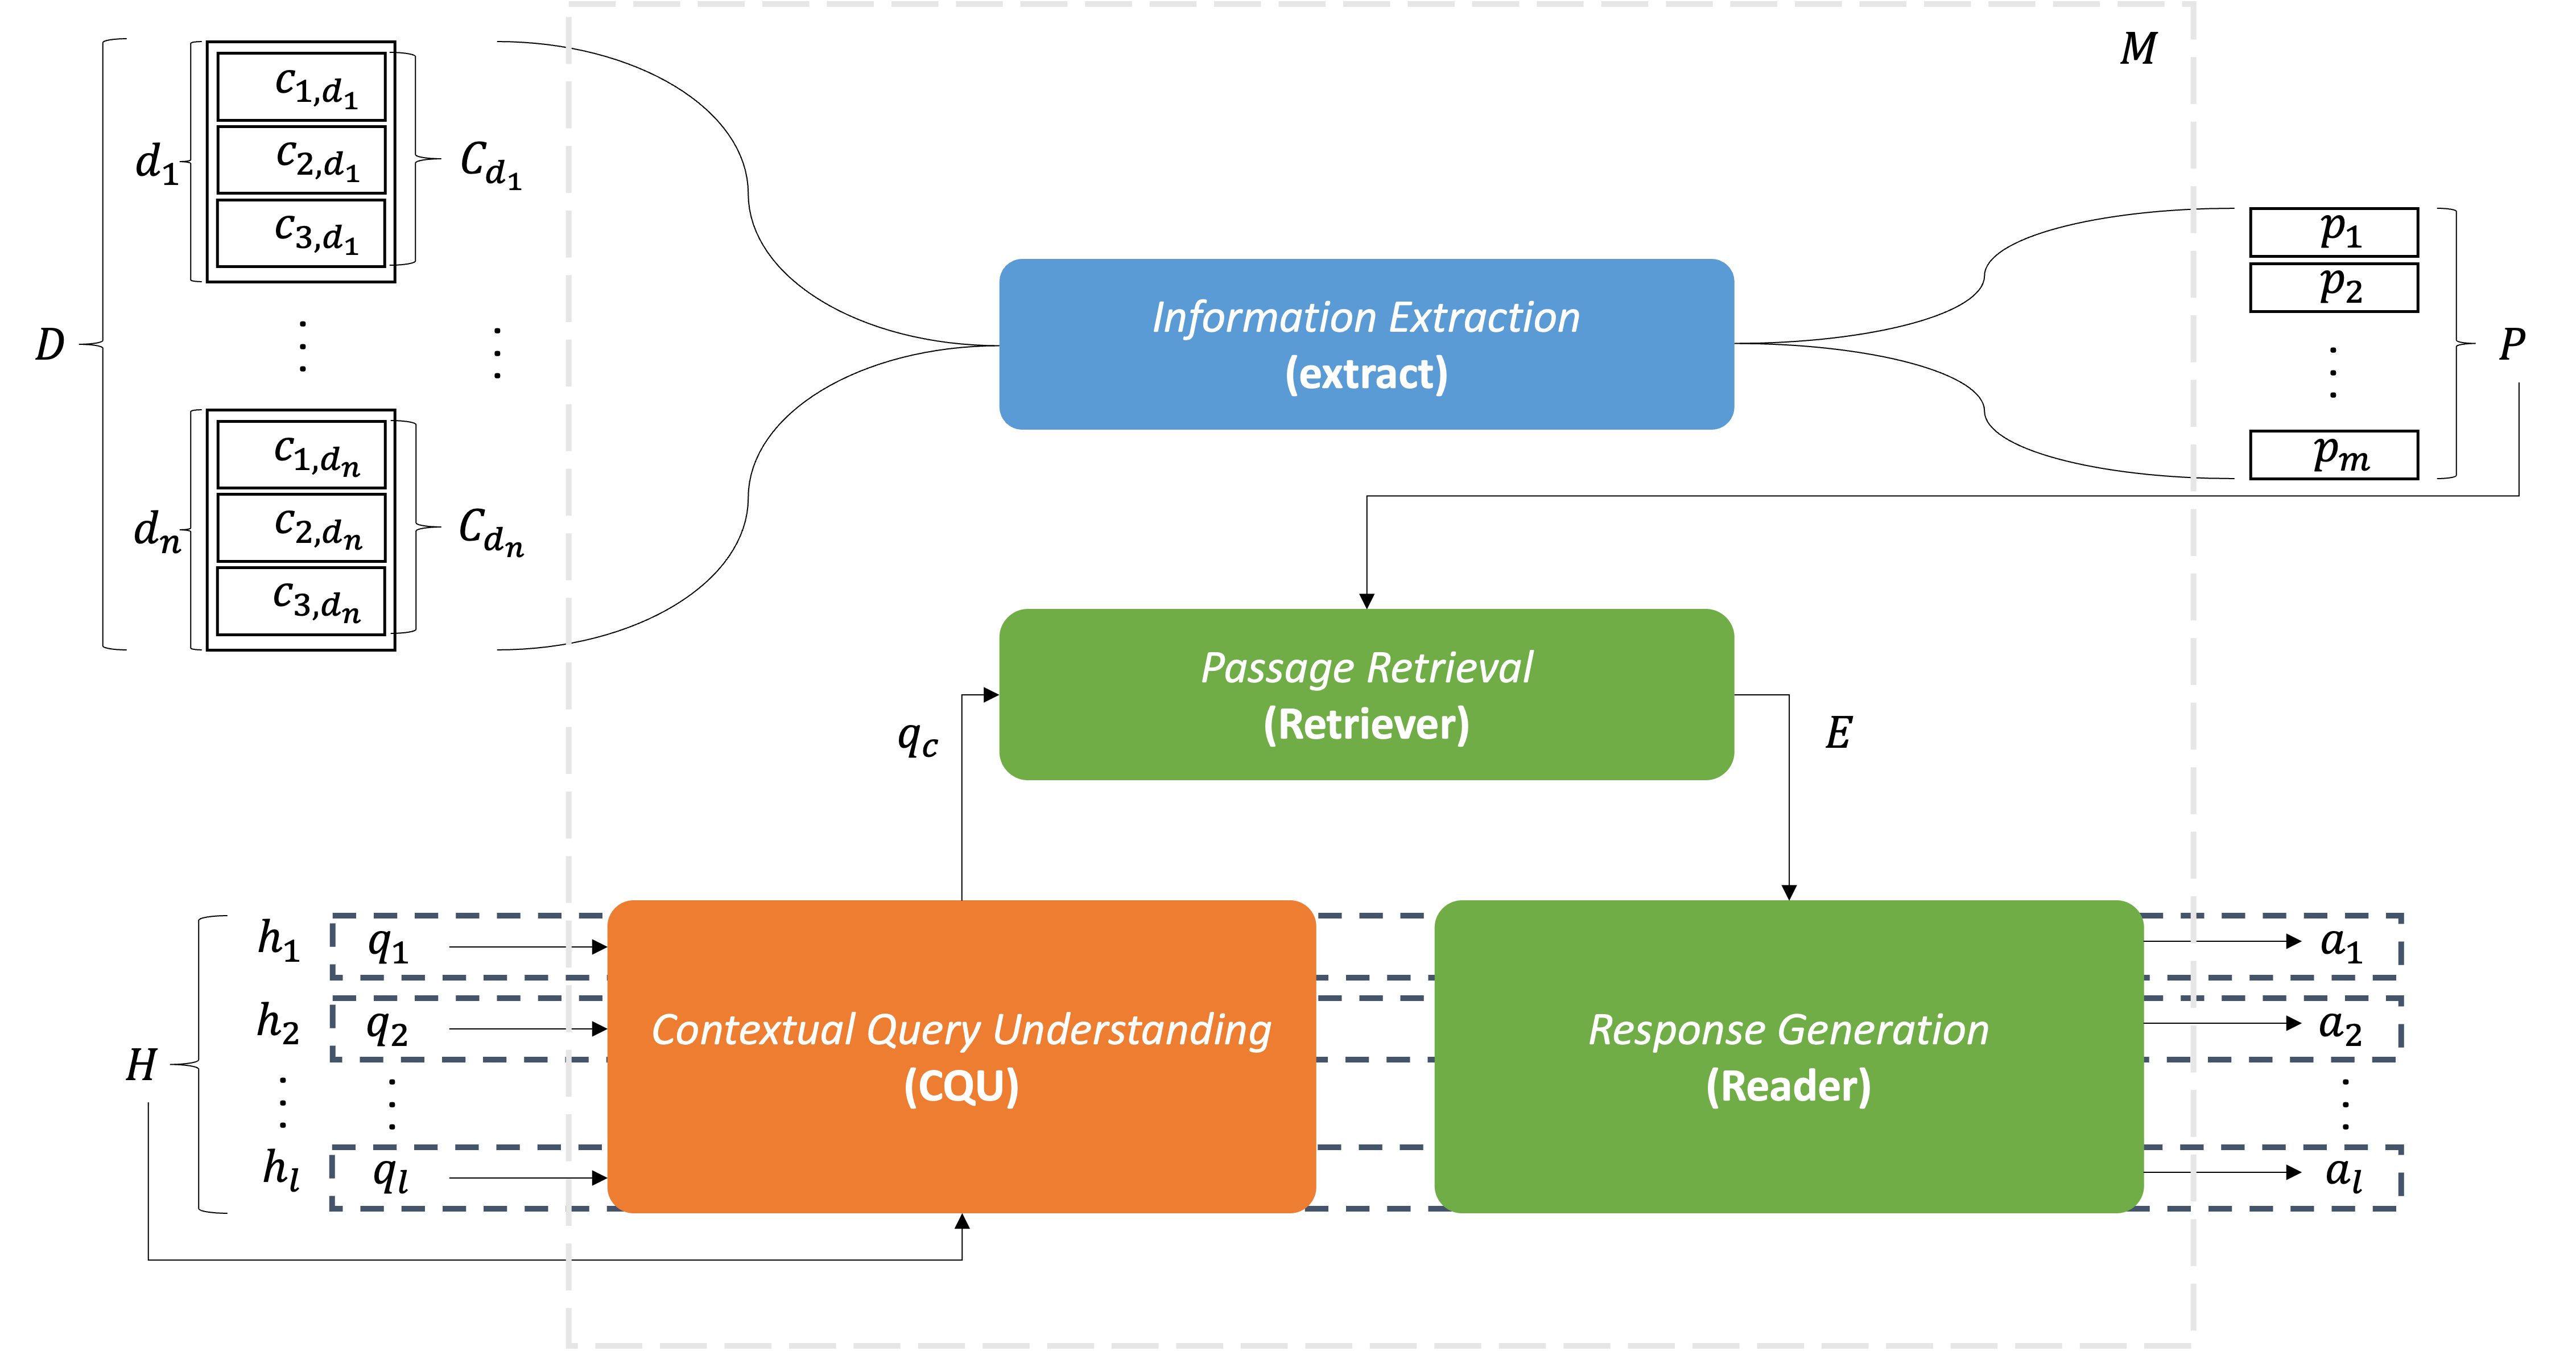
\includegraphics[width=0.8\textwidth]{Grafiken/conrag_konzeptionell.png}
    \caption{Overview of the System Architecture in context of the sub-tasks of $M$}
    \label{fig:conrag_concept_system_architecture}
\end{figure}

Figure \ref{fig:conrag_concept_system_architecture} illustrates the combination of the four components, which make up the model $M$ in their corresponding sub-tasks. This is the abstract Model $M$ which leads, when applied to a real use-case, to the \gls{conrag} system architecture.

% In relation to related work, for some of these sub-tasks, there are already existing components/models, which fullfill this tasks. \textit{Information Extraction} is a well researched field, with many different approaches and models as outlined in Section \ref{subsec:qa_indexing}. Section \ref{subsec:extract} will delve into the details of this sub-task in this context. \textit{Passage Retrieval} and \textit{Response Generation} are commonly implemented as Retriever-Reader Systems as outlined in Section \ref{sec:qa}, nevertheless for this thesis, we will narrow the focus down on \gls{rag} Systems only, as they gained a lot of attention in the last year of research. Details of a both retriever and reader for this specific task will be\textit{Contextual Question Understanding} is a less researched field, with only a few approaches and models.

% This excludes fully generative Models, which can only propose an answer $a$ based on their parametric knowledge. Therefore, the system architecture will have to be based on a Retriever-Reader Architecture. In a Retriever-Reader Architecture, the Retriever identifies important passages $p$ from the knowledge source $P$ given a question $q$ (See Section \ref{subsec:qa_architectures}).

% In the following section, we will outline the general problem field of \gls{convqa}. Unlike other definitions of this problem field, our definition begins with a collection of documents $d \in D$, where \textit{document} refers to any textual knowledge source (e.g., plain text, web pages, etc.). The core task of \gls{convqa} can be defined as follows:

% \begin{definition}
%     \textbf{(\gls{convqa} Task)} The task comprises (i) information extraction, (ii) passage retrieval, (iii) response generation, and (iv) question understanding.
%     \label{def:task}
% \end{definition}

% The system architecture \gls{conrag}, introduced in Section \ref{sec:overview} (see Figure \ref{fig:convqa_system_architecture}), divides these four tasks among four components. Each of these sub-tasks corresponds to a different mechanism of the model ($M$), which is designed to engage in a conversation with a user over a collection of documents $D$. The first task (i) of extraction can be defined as follows:

% \begin{definition}
%     \textbf{(extraction)} An extraction model ($Ext$) is a model which extracts passages from a collection of documents $D$.
%     \begin{align*}
%         \mathbf{Ext: D \rightarrow P}
%     \end{align*} 
%     Whereas $P$ is a set of passages $p \in P$ and $\forall d \in D, \exists p \in P : p \subseteq d$.
%     \label{def:extraction}
% \end{definition}

% Therefore, the input to the next component of $M$, the Retriever $p_\eta(p|q)$, is as follows:

% \begin{equation}
%     \text{Input} = (Q, P) :
%     \begin{cases}
%         \begin{aligned}
%             &\text{question}, && Q = \{q_1, \ldots, q_m\} \\
%             &\text{knowledge source}, && P = \{p_1, \ldots, p_n\}
%         \end{aligned}
%     \end{cases}
% \end{equation}

% This means that the input is a tuple $(Q,P)$ consisting of a set of questions $Q = \{q_1, q_2, \ldots, q_m\}$ and a knowledge source $P = \{p_1, p_2, \ldots, p_n\}$. Therefore, the task of $p_\eta(p|q)$ with parameters $\eta$ can be defined as follows:

% \begin{definition}
%     \textbf{(Passage Retrieval)} A retrieval model ($p_\eta(p|q)$) is a model that generates a relevance score for every tuple $(q,p)$.
%     \begin{align*}
%         \mathbf{p_\eta(p|q) = Score(q,p)}
%     \end{align*}
%     Here, $q$ itself is a tuple $(q,i)$, where $i \in I$, and $I$ is the set of all possible search intents. 
%     \label{def:retrieval}
% \end{definition}

% The set of search intents $I$ (e.g., extractive, abstractive, etc., see Section \ref{subsec:cqa_basics}) is finite. The index $i$ of a question $q$ is implicit and therefore not further specified in the following notations. Hence, instead of representing the whole tuple as $(q,i)$ for each question, we simplify it to just $q$. Task (iii) of response generation is carried out by a generator/reader $p_\theta(a|q,p)$ with parameter $\theta$:

% \begin{definition}
%     \textbf{(Response Generation)} A generation model ($p_\theta(a|q,p)$) is a model that generates an answer $a$ given a question $q$ and top-$k$ retrieved passages $p$.
%     \begin{align*}
%         \mathbf{p_\theta(a|q,p) = a}
%     \end{align*}
%     \label{def:generation}
% \end{definition}

% In a more general context, we assume that there always exists a correct answer $a$ to a question $q$ that can be extracted from the passages $P$. Therefore, we distinguish the following cases:

% \begin{equation}
%     \forall q \in Q, \exists! a \in A : a = 
%     \begin{cases}
%         \begin{aligned}
%             &1. \text{ } f(q, \emptyset), \text{ } &\text{if there is no evidence in } P \\
%             &2. \text{ } f(q, p), \text{ } &\text{if there is exactly one piece of evidence in } P \\
%             &3. \text{ } f(q, E) \mid E \subset P, \text{ } &\text{if there are multiple pieces of evidence in } P
%         \end{aligned}
%     \end{cases}
% \end{equation}

% In case 1, the answer $a$ to the question $q$ indicates that there is no evidence available for this question. Depending on the specific question $q$ intend $i$, this can lead to different answers. Case 2 can be an example of a common extraction question $q$ where the answer $a$ refers to an exact span in one passage $p$. Case 3 involves more complex questions $q$ that require information from multiple passages $p$ to be answered correctly.

% Lastly, task (vi) is handled by a \gls{cqu} $p_\xi(q_c|H,q_i)$ with parameter $\xi$:

% \begin{definition}
%     \textbf{(Question Understanding)} A question understanding model ($p_\xi(q_c|H,q_i)$) is a model that generates a contextualized question $q_c$ given a history $H$.
%     \begin{align*}
%         \mathbf{p_\xi(q_c|H, q_i) = q}
%     \end{align*}
%     Contextualized refers to identifying language-specific features between turns of a conversation to incorporate the context of the conversation into the question $q_i$.
%     \label{def:question_understanding}
% \end{definition}

% The history $H$ is further described in Section \ref{subsec:cqa_basics}.

% Figure \ref{fig:task_convqa} illustrates the general task of \gls{convqa}. It displays the relationship between questions, answers, documents, and the model $M$ on a high level. The following sections will delve deeper into the individual components of $M$. Section \ref{subsec:extract} will discuss sub-task (i), Section \ref{subsec:retriever} will discuss sub-task (ii), Section \ref{subsec:reader} will focus on sub-task (iii), and Section \ref{subsec:cqu} will explore sub-task (vi).

% \begin{figure}
%     \centering
%     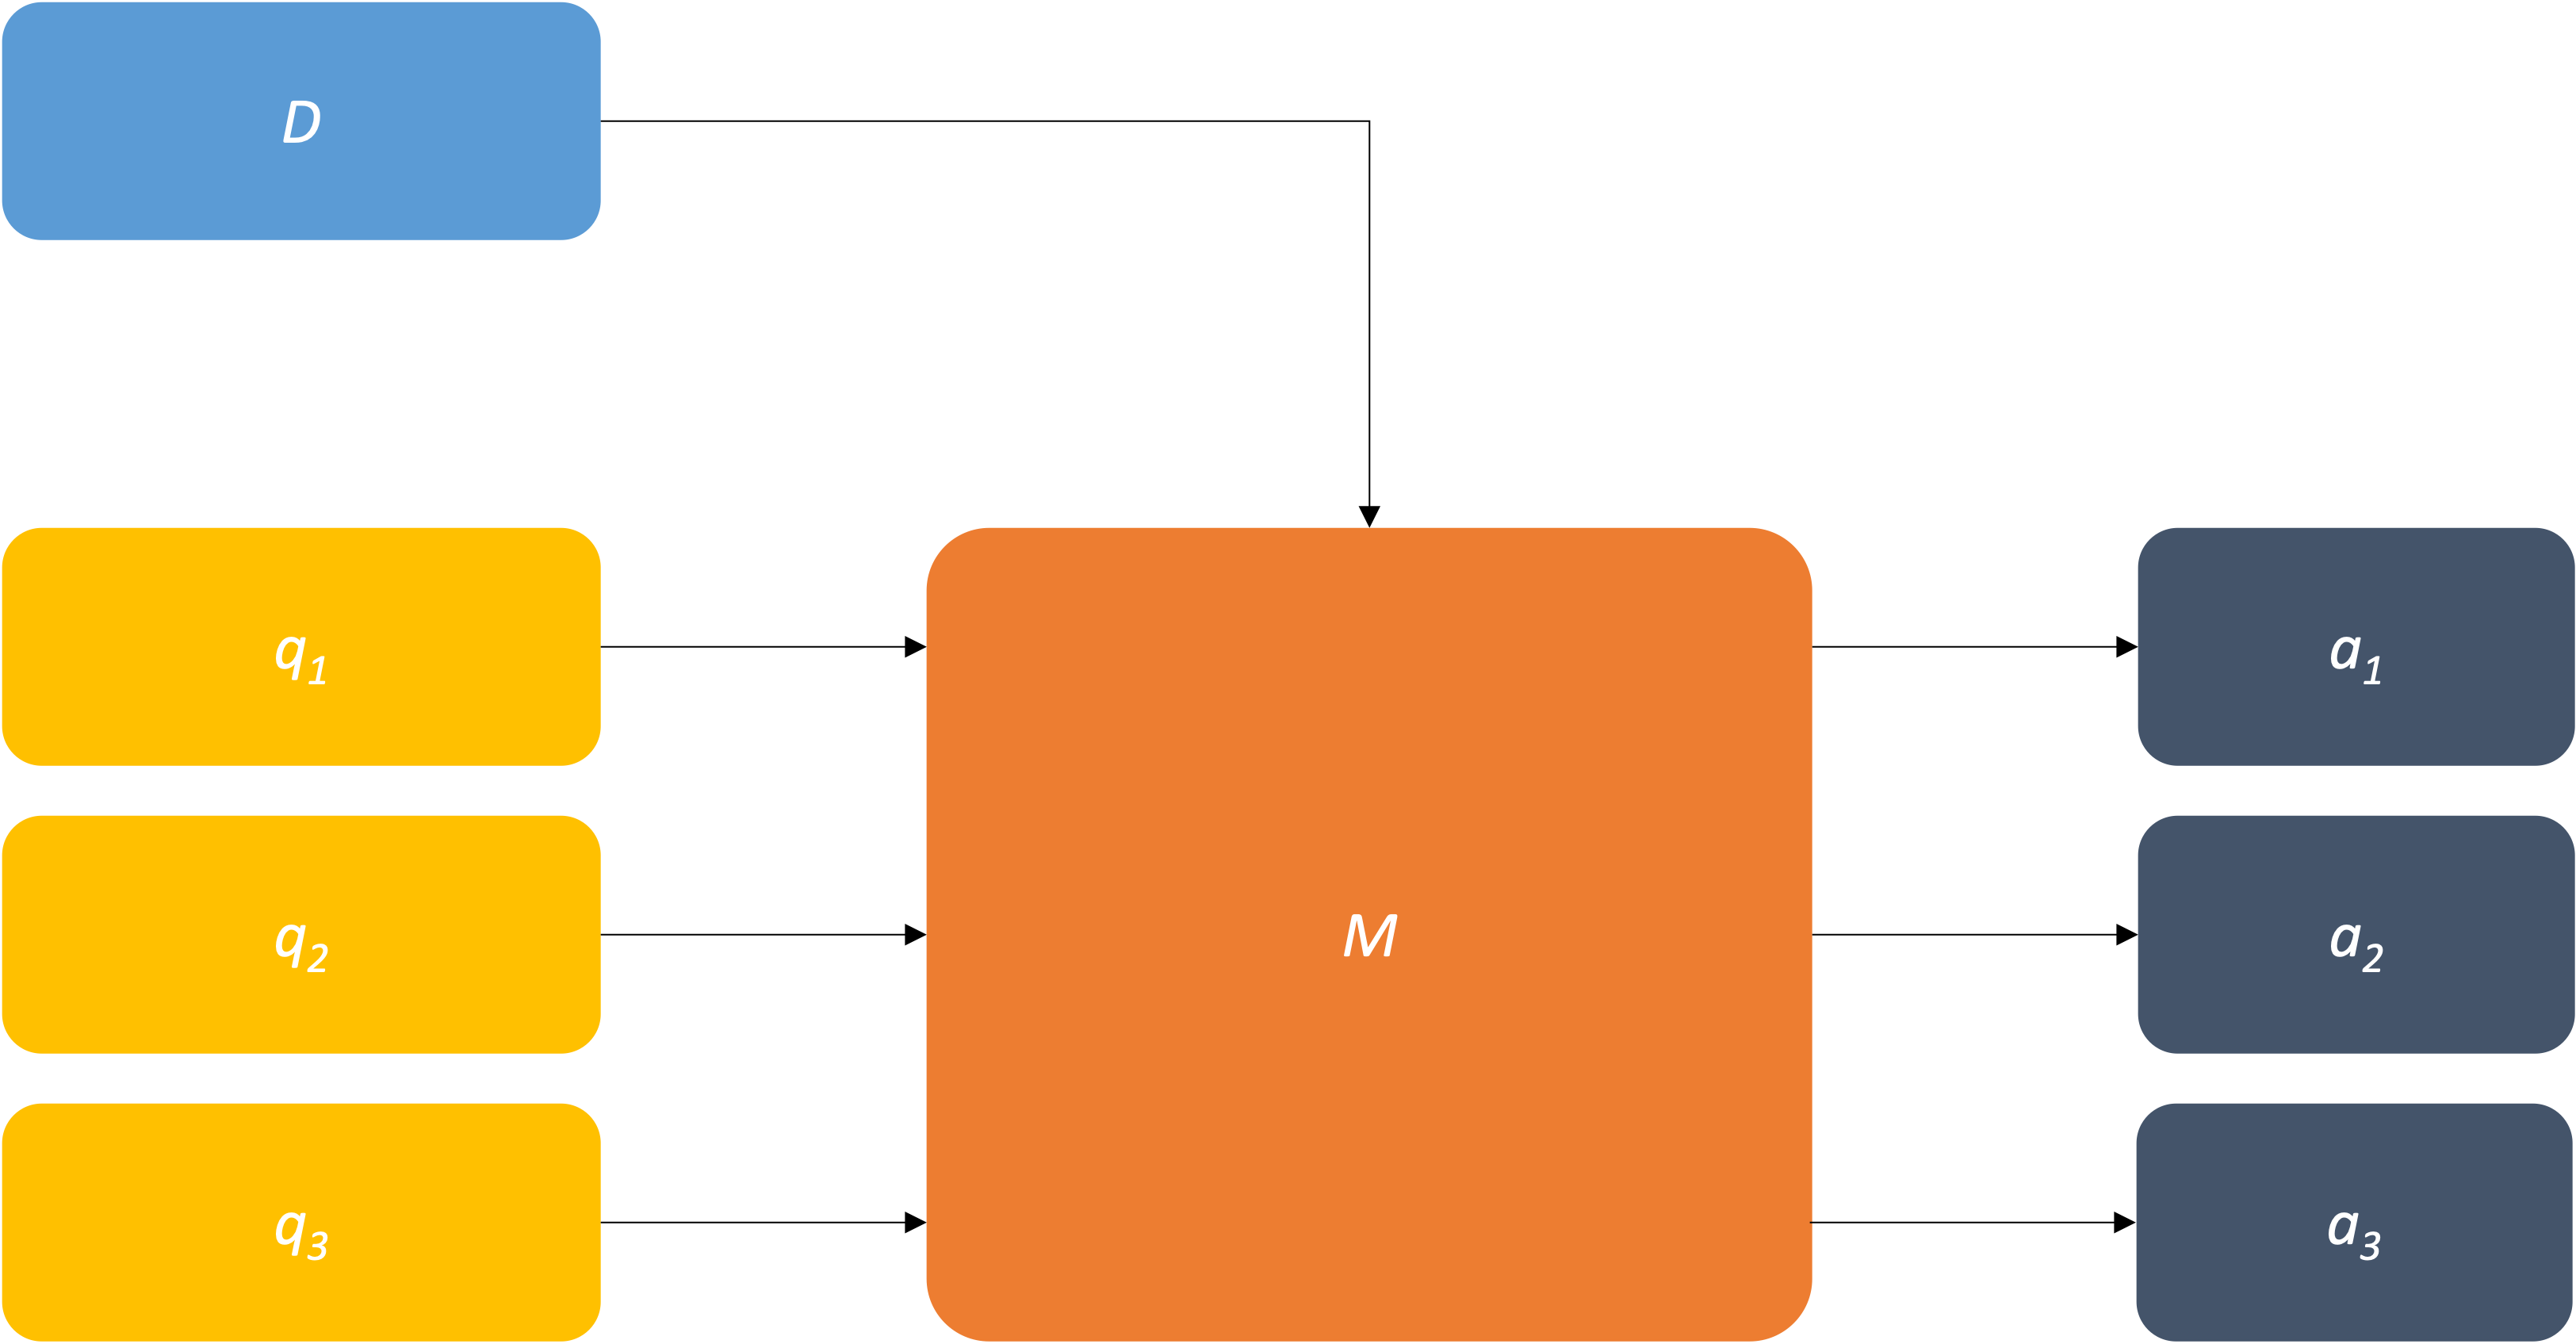
\includegraphics[width=0.8\textwidth]{Grafiken/general_conqa.png}
%     \caption{General Task of \gls{convqa}}
%     \label{fig:task_convqa}
% \end{figure}


% As illustrated in Figure \ref{fig:overview-system-architecture}, it is logical to partition the extensive grid of possibilities into smaller, manageable components that can be explored and designed independently. Consequently, the framework will be divided into two main segments: the extraction pipeline, with its potential configurations outlined in Figure \ref{fig:extract_pipeline}, and the three major modules: Retriever, Reader, and \gls{cqu}, showcasing their possible implementations in Figure \ref{fig:all_components_conrag}.

% \begin{figure}
%     \centering
%     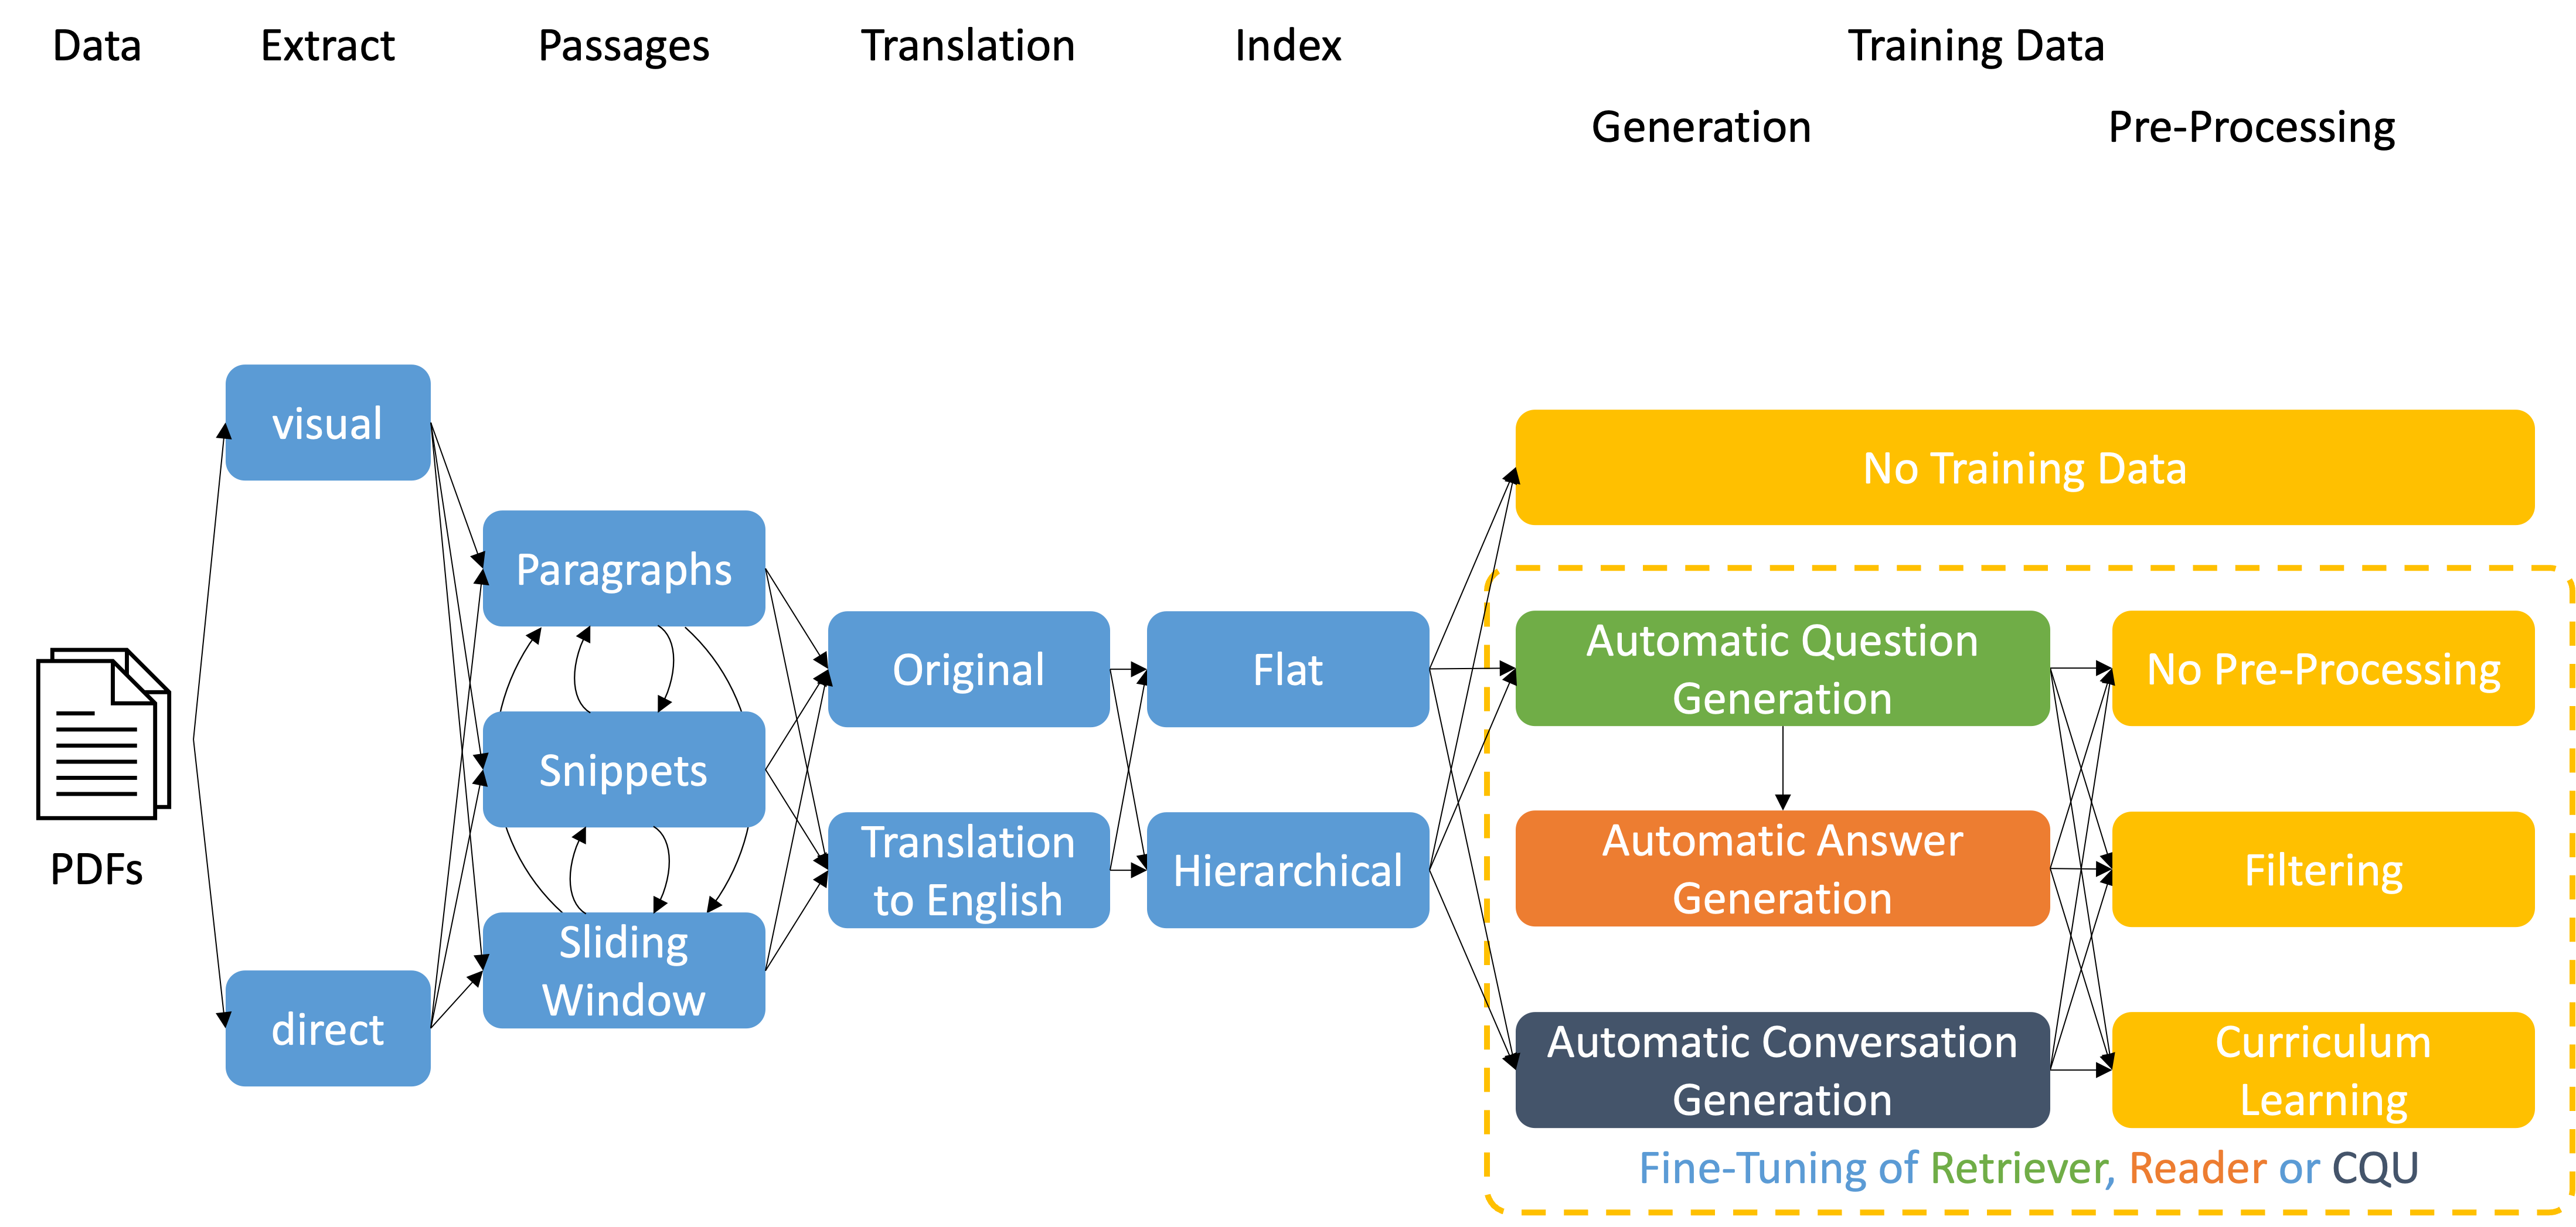
\includegraphics[width=\textwidth]{Grafiken/extract_pipeline.png}
%     \caption{Overview of the Extraction Pipeline Framework}
%     \label{fig:extract_pipeline}
% \end{figure}

% The framework varies in its level of granularity, shifting between high-level concepts and precise details. This is primarily due to the fact that certain aspects of the framework are well-researched and represent state-of-the-art knowledge, while others are ongoing research and necessitate a more abstract, conceptual treatment. For instance, \textit{BM25} is mentioned specifically as the state-of-the-art Sparse Retriever within the Retriever Module, whereas \textit{Automatic Question Generation} in the Training Data Generation step of the extraction pipeline is presented as a high-level concept.

% The framework strives to maintain a high level of generality, intentionally avoiding the incorporation of restrictive paradigms, except for the specified system architecture of \gls{rag} for \gls{qa}. This decision is motivated by the breakthroughs and extensive research endeavors within the field of \gls{llm}s, as exemplified by the exceptional success of \textit{ChatGPT}. In response to the limitations of ChatGPT, including \textit{hallucination}, \textit{implicit knowledge}, and \textit{static knowledge}, interest has surged in the \gls{rag} architecture as a means to address these issues. Presently, there is no existing survey or similar resource that provides a quantitative evaluation of the ongoing business initiatives aimed at implementing RAG-based Systems. Nonetheless, both Google Cloud Services \cite{noauthor_generative_nodate} and Amazon Web Services \cite{noauthor_quickly_2023} have introduced new services that empower customers to construct \gls{rag}-based systems, with Langchain serving as the Framework for the Reader Implementation \cite{noauthor_langchain-ailangchain_nodate}. Consequently, the framework presented here seeks to illuminate potential pathways for implementing a \gls{conrag} system, as depicted in Figure \ref{fig:convqa_system_architecture}, tailored to the use case described in Section \ref{sec:overview}.

% The extraction pipeline can be visualized as a tree, where following different paths signifies making decisions with corresponding implications for subsequent steps and components. In Figure \ref{fig:all_components_conrag}, each column represents a decision to be made, although in some cases, choosing not to decide is itself a decision. Dotted lines encircling multiple frames indicate that a combination or ensemble approach is possible. For a better understanding of how to apply this framework to create a potential system implementation, refer to the example in Figure \ref{fig:example_decission_tree}. As previously mentioned, the framework does not prescribe specific models (e.g., BERT, PaLM, etc.) but rather conceptual approaches (e.g., Cross-Encoder). The example in Figure \ref{fig:example_decission_tree} represents a simple zero-shot baseline, which will also be implemented and tested in this thesis Chapter \ref{chap:eval}.

% \begin{figure}
%     \centering
%     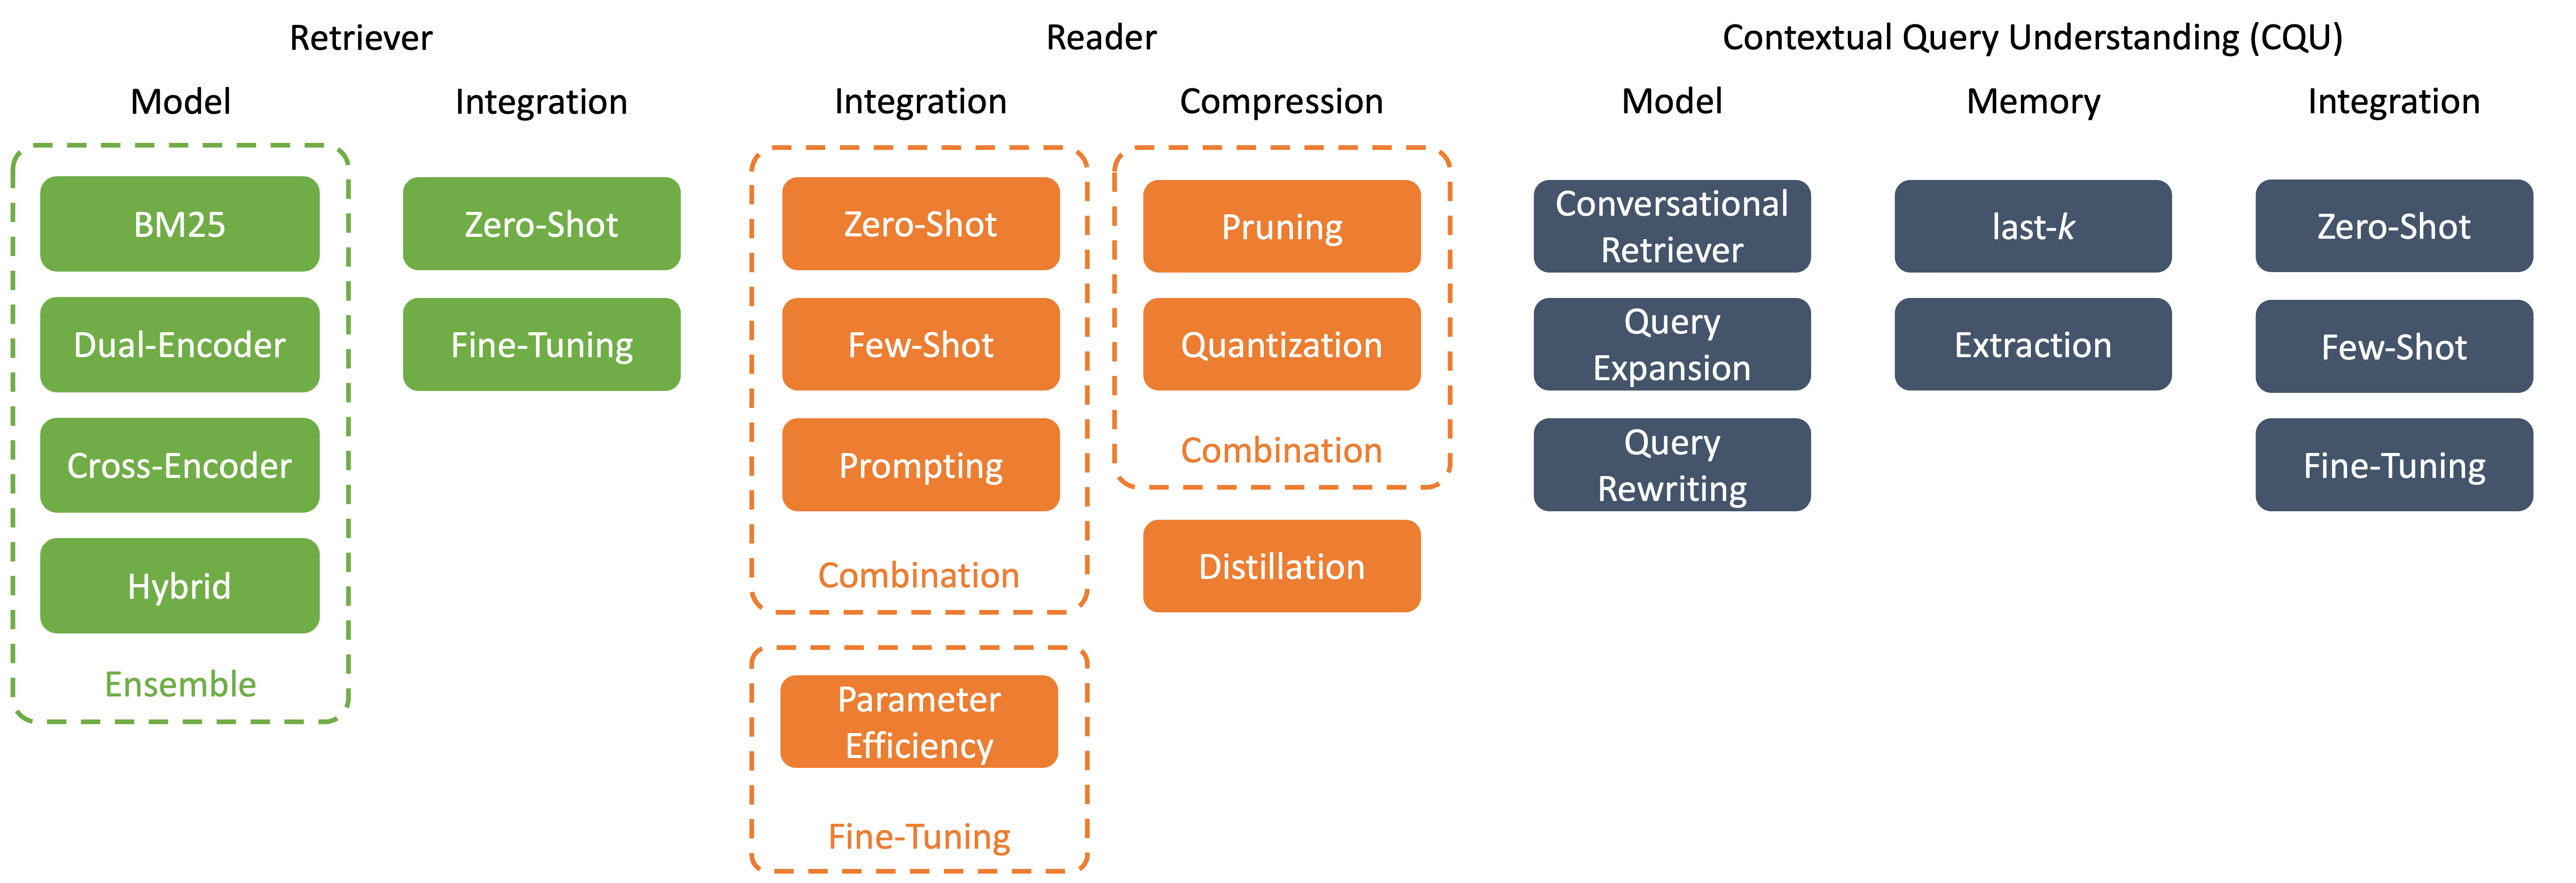
\includegraphics[width=\textwidth]{Grafiken/all_components_conrag.png}
%     \caption{Overview of all Modules of the Framework}
%     \label{fig:all_components_conrag}
% \end{figure}

% \begin{figure}
%     \centering
%     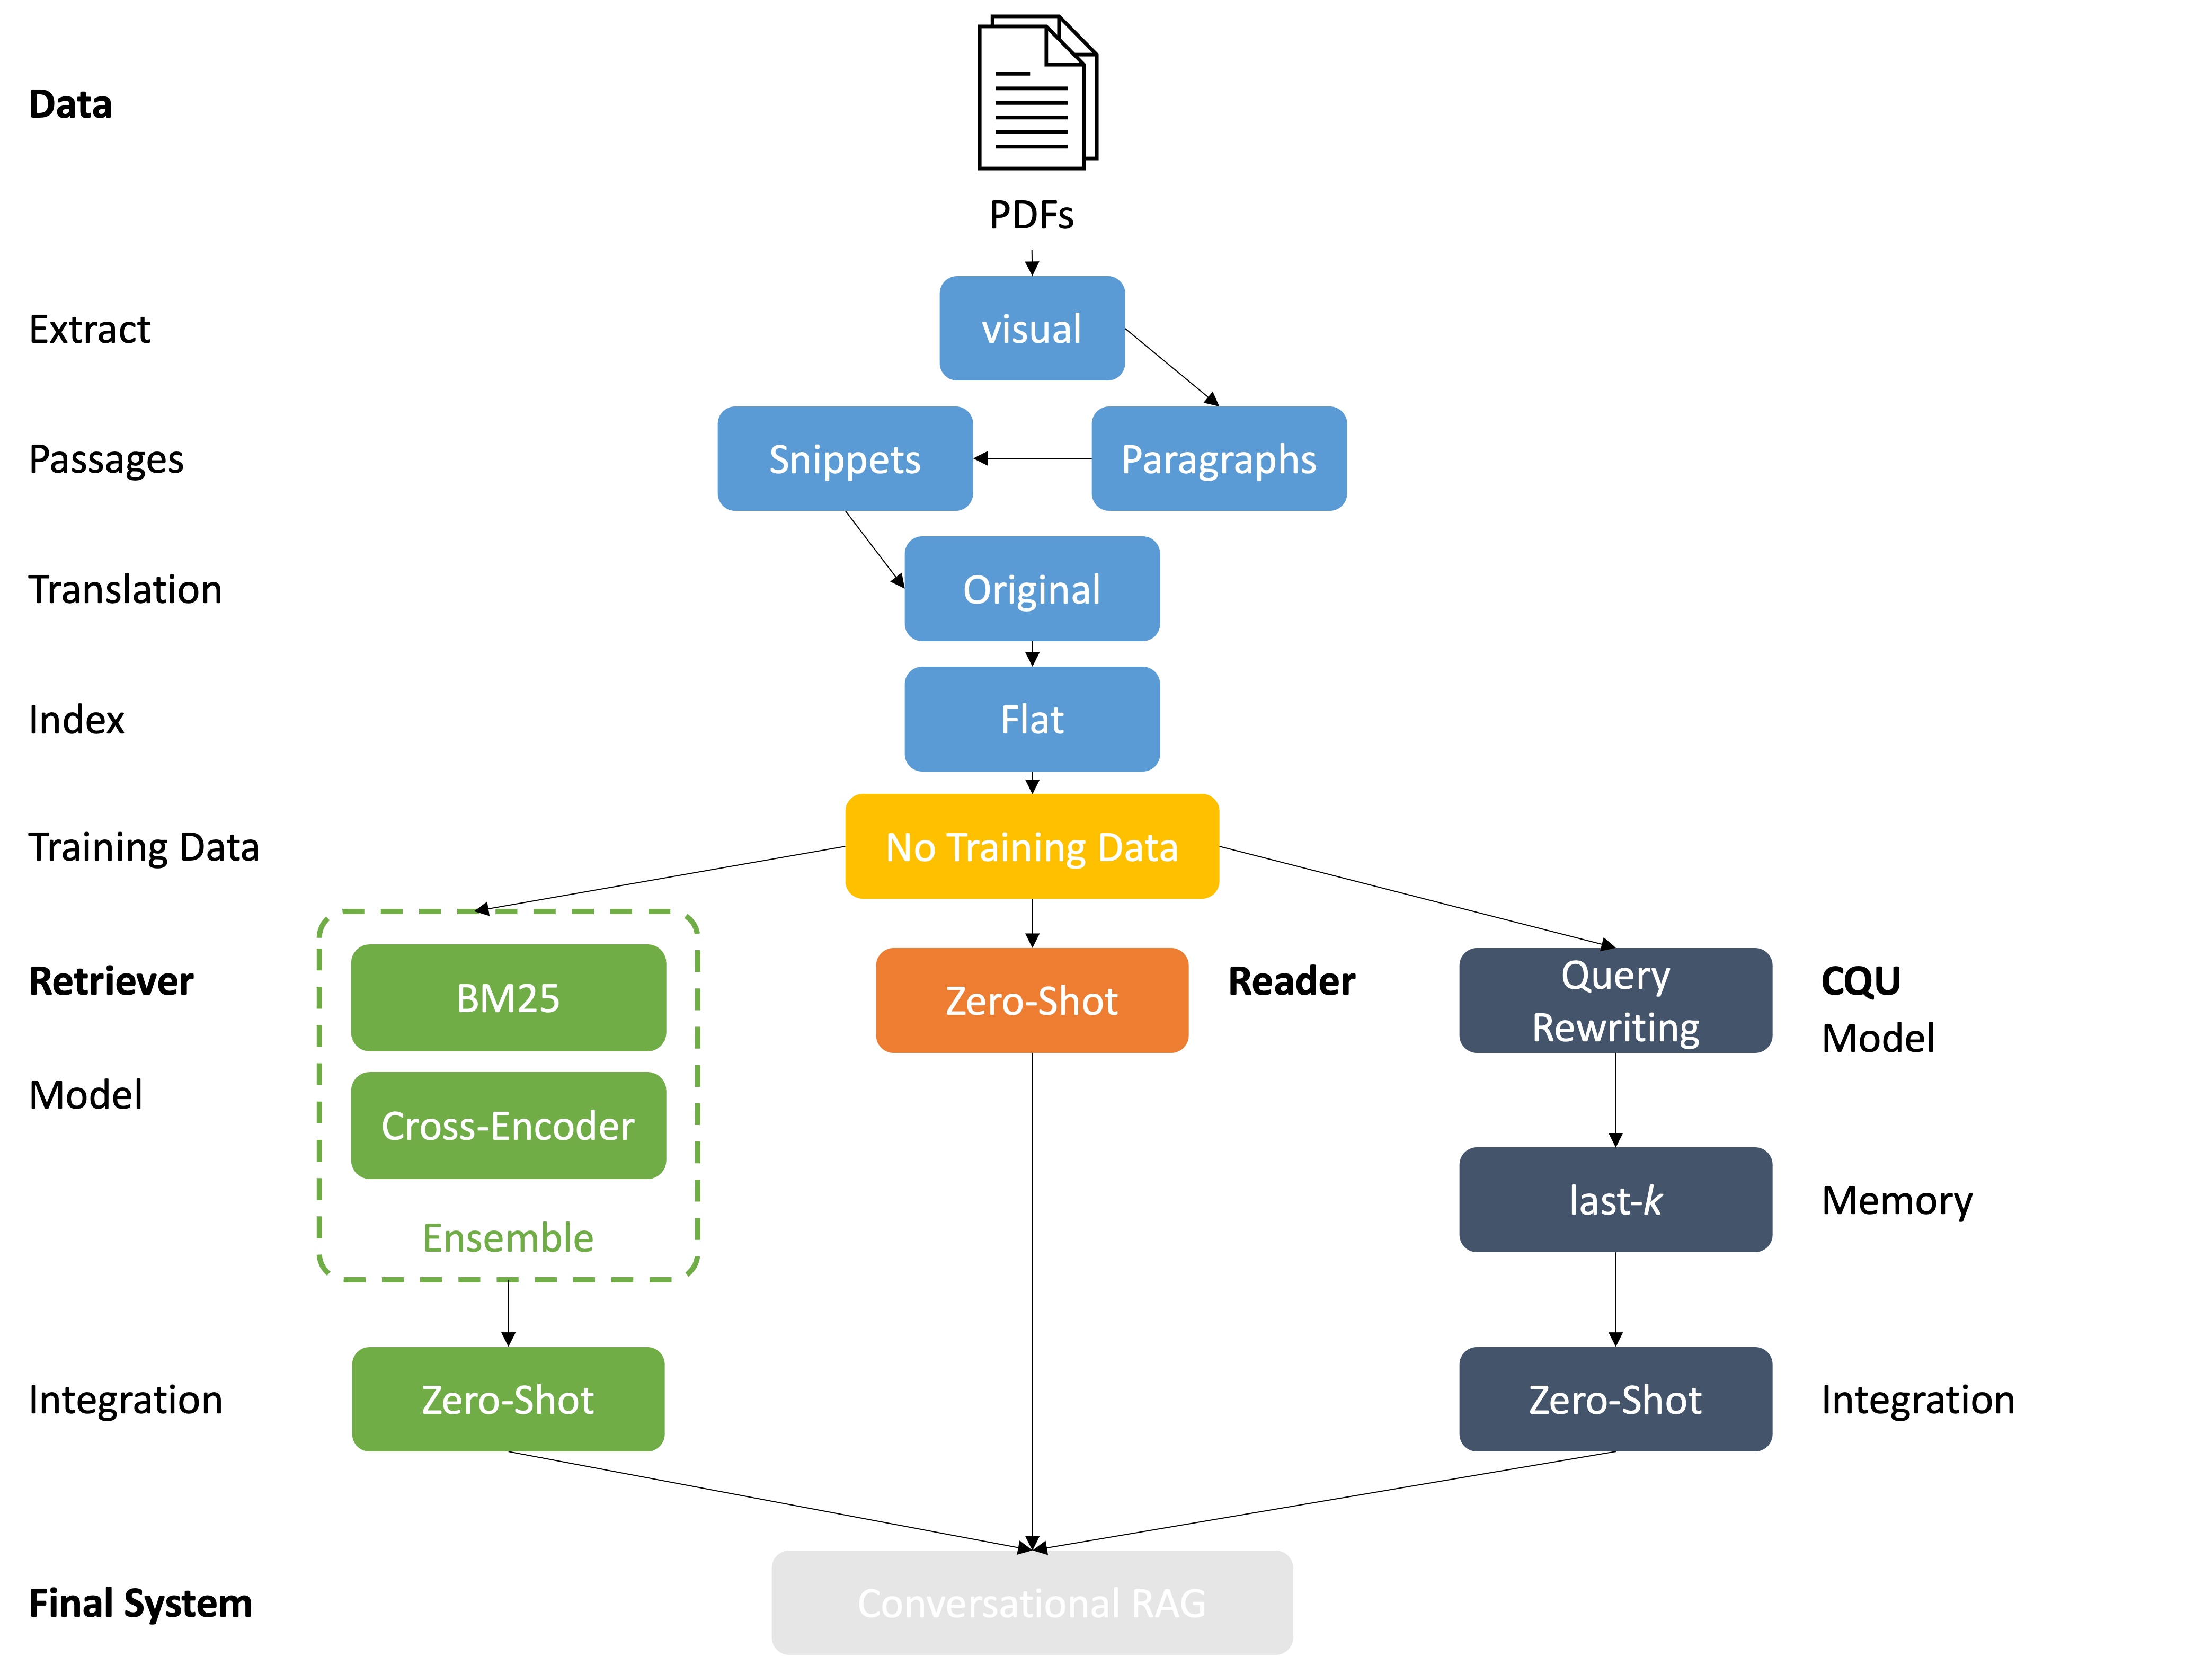
\includegraphics[width=\textwidth]{Grafiken/example_decission_tree.png}
%     \caption{Example of applying the Framework to a System Implementation}
%     \label{fig:example_decission_tree}
% \end{figure}



\subsection{extract}
\label{subsec:extract}

The sub-task of \textit{Inforamtion Extraction} was defined in the previous Section as sub-task (1) of the model $M$. Given a set of documents $D$, the knowledge source $P$ needs to be extracted using \textit{Information Extraction} techniques in combination with \textit{Passage Extraction} operations. As synthetic data generation is also part of the extraction component according to Section \ref{sec:overview}, it will also be discussed in this section. This is originally not part of the model $M$, but makes from a system architecture sense, to place these operations in this system component. Synthetic Data can be seen as an seperate task, which has nothing to do with the original task of \gls{convqa}, but is a necessary step in order to train components of the model $M$ or evaluate those.

\vspace{\baselineskip} % Add one line space

\textbf{Information Extraction:} When it comes to extracting text from any document $d$, there are many approaches to choose from. Some extract structures, metadata, or similar, which can be further utilized, while others extract unstructured text only. In any case, this extraction process highly depends on the source document type. An HTML website requires different approaches and tools compared to a PDF, for instance. An example tool for direct extraction of PDFs is Py2PDF \cite{noauthor_welcome_nodate}. Regardless of the source document and tool used to extract textual information $C_d$, there are two major possible outcomes given a set of documents $D$:

\begin{enumerate}
    \item \textit{Structured Extraction:} Denoted as $f_{StrucExt}(\cdot)$, in this extraction operation, $C_d$ can be extracted into logical segments directly: $f_{StrucExt}(d) = \{c_{d_i} \subseteq C_d : i \in \{1, 2, \ldots, n\}, C_d = \bigcup_{i=1}^{n} c_{d_i}\}$. If $f_StrucExt$ is applied to all documents $d$ in $D$, the resulting set $C$ contains all the outputs of $f_{StrucExt}$ for each document in $D$. Formally, $f_{StrucExt}(D) := C = \{C_{d_1}, C_{d_2}, \dots, C_{d_m}\}$, where each document $d$ is transformed into a set of logical segments $C_{d_i}$ representing its content.
    \item \textit{Unstructured Extraction:} Denoted as $f_{UnstExt}(\cdot)$, when applied to $D$, it results in a concatenated text corpus $C_d = \{c_d\} $ containing the textual content of a document $d$: $f_{UnstExt}(D) := C = \{C_{d_1}, C_{d_2}, \dots, C_{d_n}\}$, where each document $d$ is transformed into a single text snippet $c_d$ representing its content.
\end{enumerate}

In order to generate now snippets $p$ from $C$, \textit{Passage Extraction} has to be applied on $C$.

\vspace{\baselineskip} % Add one line space

\noindent\textbf{Passage Extraction:} The implementation of passage splitting depends on the nature of $C$ and the desired granularity of the output. In general, there are three operations for constructing passages $p$ based on a text snippet $c_d$:

\begin{enumerate}
    \item \textit{Paragraphs:} $f_p(\cdot)$ is an operation that transforms a collection $C_d$ of texts $c_d$ into a set of passages $P = \{p_1, p_2, \dots, p_n\}$. It operates similarly to $f_{StrucExt}(\cdot)$, but instead of $D$, it operates on $C_d$. The output of $f_p(\cdot)$ consists of passages $p$ that represent logical segments of the text corpus $c_d$. Usually, it operates in a \textit{rule-based} manner, meaning that a paragraph is defined by a token indicating a paragraph (e.g., \textit{<p/>} in HTML). The length $l$ of each $p_i$ is variable, and the number of paragraphs $|P|$ can also vary.
    \item \textit{Snippets:} $f_s(\cdot)$, when you have a fixed passage length $l$, divides the concatenated text $c_d$ into $|c_d|\bmod{l} + 1$ passages $p$ per $c_p$. Alternative approaches may involve specifying minimum and maximum lengths, denoted as $l_{\text{min}}$ and $l_{\text{max}}$. The exact point of division depends on whether a sentence ends within the specified window or not. If a sentence ending is found within the window, the snippet concludes at that point. Otherwise, it concludes at the end of the window. The individual length of the extracted passages $P = \{p_1, p_2, \ldots, p_n\}$ is not fixed in the case of syntactic snippets, as well as the number of paragraphs $|P|$.
    \item \textit{Sliding Windows:} $f_w(\cdot)$ utilizes a window size $l$, a concatenated text $c_d$, and a step size $s$. The window slides over the text $c_d$, and the text within the window is used as a passage $p$. This results in $\frac{|c_d| - l}{s}$ passages, denoted as $P = \{p_1, p_2, \ldots, p_n\}$.
\end{enumerate}

These operations can be combined in a pipeline fashion. For example, first $f_p(C_d) := P_{paragraphs} = \{p_{paragraphs,1}, p_{paragraphs,2}, \dots, p_{paragraphs,n}\}$ is constructed, and afterwards, on the logical paragraphs, $f_w(f_p(C_d)) := f_w(P_{paragraph}) = P_{window} = \{p_{window,1}, \allowbreak p_{window,2}, \allowbreak \dots, p_{window,i}\}$ is applied. The way these operations are combined is highly use-case specific and needs to be evaluated for each use-case individually. Another important factor influencing the decision regarding the parameters $l$ and, in general, the operation used, is the desired model for the \textit{Retriever} and \textit{Reader} as they may be trained on a specific token length as input or have a maximum length of tokens they accept as input or require a certain clarity of data points.


\vspace{\baselineskip} % Add one line space
\noindent\textbf{Synthetic Training Data Generation:} This can be interpreted as a knowledge distillation task. The main idea is to use a model $ED(\cdot)$ to generate a synthetic dataset for the sub-task and problem field of \textit{Passage Retrieval} and \textit{Response Generation}:

\begin{equation}
    \mathbf{ED(P) := (P, Q, I)}
    \label{eq:task}
\end{equation}

Where $P = \{p_1, p_2, \dots, p_n\}$ corresponds to a corpus of passages to retrieve from, $Q$ is a set of questions, and $I$ is the underlying search intent for a question $q \in Q$. If $I(q,p) = 1$, this means that the passage reflects the question's search intent. Given this task, there are several synthetic dataset types:

\begin{enumerate}
    \item \textit{Questions given Context} $ED_{qgp}(p,I) := q_s$: Given a passage $p$, generate a synthetic question $q_s$ that satisfies the desired search intent $I$. Applying $ED_{qgp}(P)$ to a set of passages will generate a set of questions $Q_s = \{q_1, q_2, \dots, q_n\}$, with one question for every passage, i.e., $|Q_s| = |P|$. $ED_{gpq}$ can also be applied multiple times with different $i \in I$ to generate multiple different questions $q_{j,s,1}, q_{j,s,2}, \dots , q_{j,s,i}$ for a single passage $p_j$.
    \item \textit{Question-Context-Answer Triples} $ED_{qpa}(p, I) := (q_s, p, a_s, I)$: Given a passage $p$, generate a synthetic question $q_s$ that satisfies the search intent $I$ and provides an answer $a_s$, where $I(q_s, a_s, p) = 1$. The result of applying $ED_{qpa}(P)$ to a set of passages is a set of question-passage-answer triples $QPA_s = \allowbreak \{(q_{1,s}, p_1, a_{1,s}, I), \allowbreak (q_{2,s}, p_2, a_{2,s}, I), \allowbreak \dots, (q_{n,s}, p_n, a_{n,s}, I)\}$, where $|QPA_s| = |P|$. $ED_{qpa}$ can also be applied multiple times with different $i \in I$ to generate multiple different questions $q_{j,s,1}, \allowbreak q_{j,s,2}, \dots , q_{j,s,i}$ and corresponding answers $a_{j,s,1}, \allowbreak a_{j,s,2}, \dots , a_{j,s,i}$ for a single passage $p_j$.
\end{enumerate}

While the previous two approaches focus on single tuples of either $(q,p)$ or triples of $(q,p,a)$, there is also a problem field of generating conversations based on passages $P = \{p_1, p_2, \dots, p_n\}$ from the same underlying document $d$. Therefore, the task given in Equation \ref{eq:task} is changed to:

\begin{equation}
    \mathbf{ED(P) := (H, P, I)}
    \label{eq:task_conversation}
\end{equation}

Where $H$ corresponds to a set of conversation histories $h$ containing multiple turns. The first turn is always a question $q_1$, followed by an answer $a_1$ based on a passage $p \in P$, also given a search intent $I$ over the whole history $h$. Synthetic datasets for this task can be generated in the following ways:

\begin{enumerate}
    \setcounter{enumi}{2} % Set the starting value to 3
    \item \textit{Conversational Question-Context-Answer Histories} $ED_{cqpa}(E, I) := H_s$: Given a subset of passages $E \subset P$, the task of the model $ED_{cqpa}$ is it to construct a realistic conversation with an intent $I$ over the corpus $E$. The result of applying $ED_{cqpa}(E,I)$ on a set of passages is a set of conversation histories $H_s = \{h_1, h_2, \dots, h_n\}$. $ED_{cqpa}$ can also be applied multiple times with different $i \in I$ in order to generate multiple different conversations $h_{j,s,1}, h_{j,s,2} \dots , h_{j,s,i}$ for a single subset of passages $E \subset P$.
\end{enumerate}

There are several ways to implemnt the models $ED_{qgp}$, $ED{qpa}$ or $ED_{cqpa}$. Implementations of those appraoches will be discussed in Chapter \ref{chap:eval}. 


% In this pipeline, the prompt-based \gls{qg} method known as PROMPTAGATOR \cite{dai_promptagator_2022} is used to generate a synthetic \gls{qa} dataset for ColBERTv2 \cite{santhanam_colbertv2_2022} based on $P$. The goal is to create triples of $(q, p^{+}, p^{-})$, similar to those found in datasets like MS MACRO \cite{bajaj_ms_2018}. For the task of $E_{qg}(p) := q$, a \gls{s2s} model, specifically a \gls{llm}, will be employed. This technique can be interpreted as knowledge distilation from the LLM to the later trained retriever. Similar to PROMPTAGATOR, there are two approaches to consider:

% \begin{enumerate}
%     \item \textit{Zero-Shot:} In this approach, a single prompt is executed to generate a question $q_i$ corresponding to a passage $p_i$, all without the need for any supervised dataset.
    
%     \item \textit{Few-Shot:} This approach uses $k$ supervised pairs $(q_j, p^{+}_{j})^{k}$ to generate a question $q_i$ corresponding to a passage $p_i \in P$.
% \end{enumerate}

% The prompt used for \textbf{zero-shot \gls{qg}}, where $p_i$ represents a passage from $P$, is:

% \verb|f'{p_i} Read the passage and generate a corresponding query.'|

% The prompt used for \textbf{few-shot \gls{qg}}, where $q_j$ represents a question, $p_j$ the corresponding passage, and $p$ the passage for which a question is being generated, is:

% \verb|f'Passage: {p_1} Question: {q_1} XXX Passage: {p_2} Question: {q_2}|

% \verb|XXX ... XXX Passage: {p} Question:'|

% The result of either of these approaches will be a synthetic training dataset of $(q_s, p^{+})$ tuples. This dataset can be used for fine-tuning the retriever.

% A major issue associated with this form of \textbf{\gls{qg}} is its strict limitation to extractive questions, where the evidence can be derived from a single passage only. This limitation significantly constrains this pipeline. However, it does not necessarily prevent the system from answering more complex questions, such as multi-hop questions. These can be addressed by the \textit{retriever} and \textit{reader} modules.


\subsection{Contextual Query Understanding}
\label{subsec:cqu}



\subsection{Retriever}
\label{subsec:retriever}

In Section \ref{sec:conrag}, we have divided the main task of a model $M$ for \gls{convqa} into multiple sub-tasks. The Retriever component handles the \textit{Passage Retrieval} task. The goal of this component is to identify relevant passages $p$ from the knowledge source $P$ given a contextualized question $q_c$. The contextualized question $q_c$ is generated by the \gls{cqu} unit (see Section \ref{subsec:cqu}). This identification includes a scoring of relevance for each passage $p$ given a question $q_c$. The scoring function $p_{\text{Ret}}(p|q_c)$ can be defined as follows:

\begin{equation}
    p_{\text{Ret}}(p|q_c) = \text{Score}(q_c,p)
    \label{eq:retriever}
\end{equation}

Here, $\text{Score}(q_c,p)$ is a value determining the relevance of a passage $p$, enabling the ranking of passages $p$ given a question $q_c$. Based on the score, the passages will be ordered in descending order, and the top-$k$ passages will be combined into an evidence set $E_{q_c}$. Within the evidence set $E_{q_c}$, a passage $p$ will be represented as a tuple $(p, \text{Score}(q_c,p))$. Concerning the evidence set $E_{q_c}$ in relation to the question $q$ and the underlying search intent $i$, the following cases exist:

\begin{equation}
    \forall q \in Q, \exists! E_{q_c} \subset P  := 
    \begin{cases}
        \begin{aligned}
            &1. \text{ } I(q,E_{q_c} = \emptyset) = 1 \\
            &2. \text{ } I(q,E_{q_c} = \{p\}) = 1 \\
            &3. \text{ } I(q,E_{q_c} = \{p_1, p_2, \dots, p_n\}) = 1
        \end{aligned}
    \end{cases}
    \label{eq:evidence_cases}
\end{equation}

For every question, there exists an evidence set. In order for intent $I(q,E_{q_c})$ to be 1, there are three cases: either the evidence set $E_{q_c}$ has to be empty, $E_{q_c}$ has to have exactly one element $p$, or $E_{q_c}$ has to have multiple passages $p$. To put it more simply, for a given question, the answer could be determined either by the evidence that there is no supporting passage $p$, or that there is exactly one passage $p$ containing the requested information, or that multiple passages $p$ contain the necessary information to answer the question $q$.

\vspace{\baselineskip}

\textbf{Retriever}: Depending on the chosen method for a Retriever, the Retriever component can either be trainable or have adjustable parameters:

\begin{align}
    r_{\text{Ret}, \theta} &= \text{Retriever}_\theta(q_c, P) \\
    r_{\text{Ret}, \Theta} &= \text{Retriever}_\Theta(q_c, P)
\end{align}

Here, $\theta$ is the set of trainable parameters, and $\Theta$ is a set of adjustable parameters. Examples of the first type of retriever include dense retrievers like \textit{\gls{dpr}}, as introduced in Section \ref{subsec:qa_retrieval}. Examples of the second type of retriever include sparse retrievers like \textit{BM25}, also introduced in the same section. Regardless of the type of retriever, the operation from Equation \ref{eq:retriever} is applied to each passage $p \in P$, and the top-$k$ passages are selected to form the evidence set $E_{q_c}$. As outlined in Equation \ref{eq:evidence_cases}, some questions may require no evidence to fulfill the search intent. However, with the proposed Retrievers, this is not possible. A retriever $r_{\text{Ret}}$ will always assign a $Score(q,p)$ to every passage given a question and its search intent. Filters could be applied to filter out passages with a low score, but this is not part of the retriever itself. The evaluation of the evidence in respect to the search intent and correctly identifying the case at hand will be handled by the Reader component (see Section \ref{subsec:reader}).

\vspace{\baselineskip}

\textbf{Mixture-of-Experts}: To enhance the quality of the evidence set $E_{q_c}$, state-of-the-art research and related work have emphasized the effectiveness of combining multiple retrievers (see Section \ref{sec:related_work}). This combination can be achieved in various ways, which can also be combined further:

\begin{itemize}
    \item \textbf{Re-Ranking}: This involves the combination of multiple retrievers in a pipeline fashion. In most cases, a fast but imprecise Retriever is used to retrieve a large evidence set, e.g., $r_{BM25}(q_c,P) = E_{q_c,1}$, where $|E_{q_c,1}| = 100$. Subsequently, a second, more accurate Retriever is employed to re-rank the evidence set $E_{q_c}$, e.g., $r_{CE}(q_c,E_{q_c,1}) = E_{q_c,2}$, where $|E_{q_c,2}| = 25$.
    
    \item \textbf{Ensemble}: This idea involves combining multiple retrievers into a single retriever. This can be accomplished by either concatenating the evidence sets $E_{q_c,j}$ or by aggregating the scores of the individual retrievers $r_j$ into a single score. Formally:
    
    \begin{align}
        \forall r \in R: E_{q_c} &= \bigcup_{j=1}^{|R|} r_j(q_c, P) \\
        \forall p \in P: \text{Score}(q_c, p) &= f(r_j(q_c, p))
    \end{align}
    
    Here, $f(\cdot)$ represents a function that combines the scores of the individual retrievers $r_j$, for example, using $max(\cdot)$, and $R$ is a set of retrievers $r$.
    
    \item \textbf{Weighting}: This approach involves running two retrievers in parallel and multiplying their scores for each passage $p$. It can be seen as a sub-case of Ensemble. Formally:
    
    \begin{equation}
        \forall p \in P: \text{Score}(q_c, p) = \prod_{j=1}^{|R|} \alpha_j \cdot r_j(q_c, p), \sum_{j=1}^{|R|} \alpha_j = 1
    \end{equation}
    
    Here, $R$ represents a set of retrievers $r_j$, and $\alpha_j$ is the weight assigned to each retriever $r_j$. These weights $\alpha_j$ can be either fixed or trainable.
\end{itemize}

\vspace{\baselineskip}

\textbf{Fine-Tuning:} Given a dataset of tuples $(q, p)$, as described in Section \ref{subsec:extract}, a retriever with trainable parameters $r_{\text{Ret}, \theta}$ can undergo fine-tuning. The first step involves creating the training data $\mathcal{TD} = \{\langle q_i, p_i^+, p_{i,1}^-, \dots, p_{i,n}^-\rangle\}_{i=1}^m$. In this dataset, we already have tuples that contain a question $q_i$ and a positive passage $p_i^+$. The primary objective is to sample $n$ negative passages $p_{i,j}^-$ for each positive passage $p_i^+$. Various methods can be employed \cite{karpukhin_dense_2020}:

\begin{enumerate}
    \item Randomly sampling passages from the knowledge source $P$, where $p_{i,j}^- \in P$ and $p_{i,j}^- \neq p_i^+$.
    \item Retrieving evidence passages using a high-performing \gls{ood} retriever $r_{\text{Ret},\text{OOD}}$ and sampling from the evidence set $p_{i,j}^- \in E_{q_i}$, ensuring $p_{i,j}^- \neq p_i^+$.
    \item Sampling passages from other tuples $(q_k,p_k)$ in the dataset, where $p_k \neq p_i^+$.
\end{enumerate}

Method (1) is the simplest but does not yield high-quality negative passages $p_{i,j}^-$. Method (2), while more complex, typically provides a higher-quality evidence set $E_{q_i}$ than method (1). Method (3) can also be applied in-batch, known as \textit{in-batch negatives}, during the training process. This means that given a batch $B$ of $|B|$-many $(q_i,p_i^+)$ tuples, the negative passages $p_{i,j}^-$ are derived from the positive passages of the other tuples in the same batch $B$. Consequently, this results in $|B| \times |B| - 1$ negative passages $p_{i,j}^-$ per batch $B$ per question $q_i$.

After construction of the training dataset $\mathcal{TD}$, the retriever $r_{\text{Ret}, \theta}$ can be trained straightforward. The forward pass is simply the score prediction of the retriever for every passage, positive and negatives, within a tuple of the $\mathcal{TD}$. Therefore the loss function can be defined as following:

\begin{equation}
    \mathcal{L}(q_i, p_i^+,p_{i,1}^-, \dots, p_{i,n}^-) = -\log \frac{e^{\text{Score}(q_i,p_i^+)}}{e^{\text{Score}(q_i,p_i^+)} + \sum_{j=1}^{n} e^{\text{Score}(q_i,p_{i,j}^-)}}
\end{equation}

The calculated loss will be used in backpropagation to update $\theta$.

The process of fine-tuning needs adaptation when using \textit{synthetically generated data} due to the potential quality issues of the synthetic dataset. To address this, the dataset must be iteratively filtered during the training process. Given a synthetic dataset $\mathcal{TD_s} = \{\langle q_i, p_i^+\rangle\}_{i=1}^m$, a retriever $r_{\text{Ret}, \theta}$ with trainable parameters $\theta$, and a high-performing out-of-domain (\gls{ood}) retriever $r_{\text{Ret},\text{OOD}}$, the following procedure is based on the proposed approach of PROMPTAGATOR \cite{dai_promptagator_2022}:

\begin{enumerate}
    \item Extend $\mathcal{TD_s}$ by adding $n$ negative passages $p_i^-$ for every tuple using Method (2) from above with $r_{\text{Ret},\text{OOD}}$.
    \item Train $r_{\text{Ret}, \theta}$ for $s$ iterations on $\mathcal{TD_s}$ while applying in-batch negatives, as described in Method (3) above.
    \item Filter $\mathcal{TD_s}$ using $r_{\text{Ret}, \theta}$ and $r_{\text{Ret}, \text{OOD}}$ by removing all tuples $(q_i, p_i^+)$ where $p_i^+$ is not in the Evidence set $E_i$, given a parameter $k$, for either $r_{\text{Ret}, \theta}$ or $r_{\text{Ret}, \text{OOD}}$.
\end{enumerate}

Figure \ref{fig:retriever-fine-tuning} illustrates the fine-tuning process with synthetic data. Steps (2) and (3) are repeated cyclically, with step (3) concluding each cycle. After $s$ epochs, $\mathcal{TD_s}$ is filtered once, retrained for $s$ epochs, refiltered, and finally trained again for $s$ epochs. This process may appear counterintuitive, as the retriever is trained on the dataset it's supposed to filter. However, experiments from related work \cite{dai_promptagator_2022} have demonstrated that this approach still yields favorable results.


\begin{figure}
   \centering
    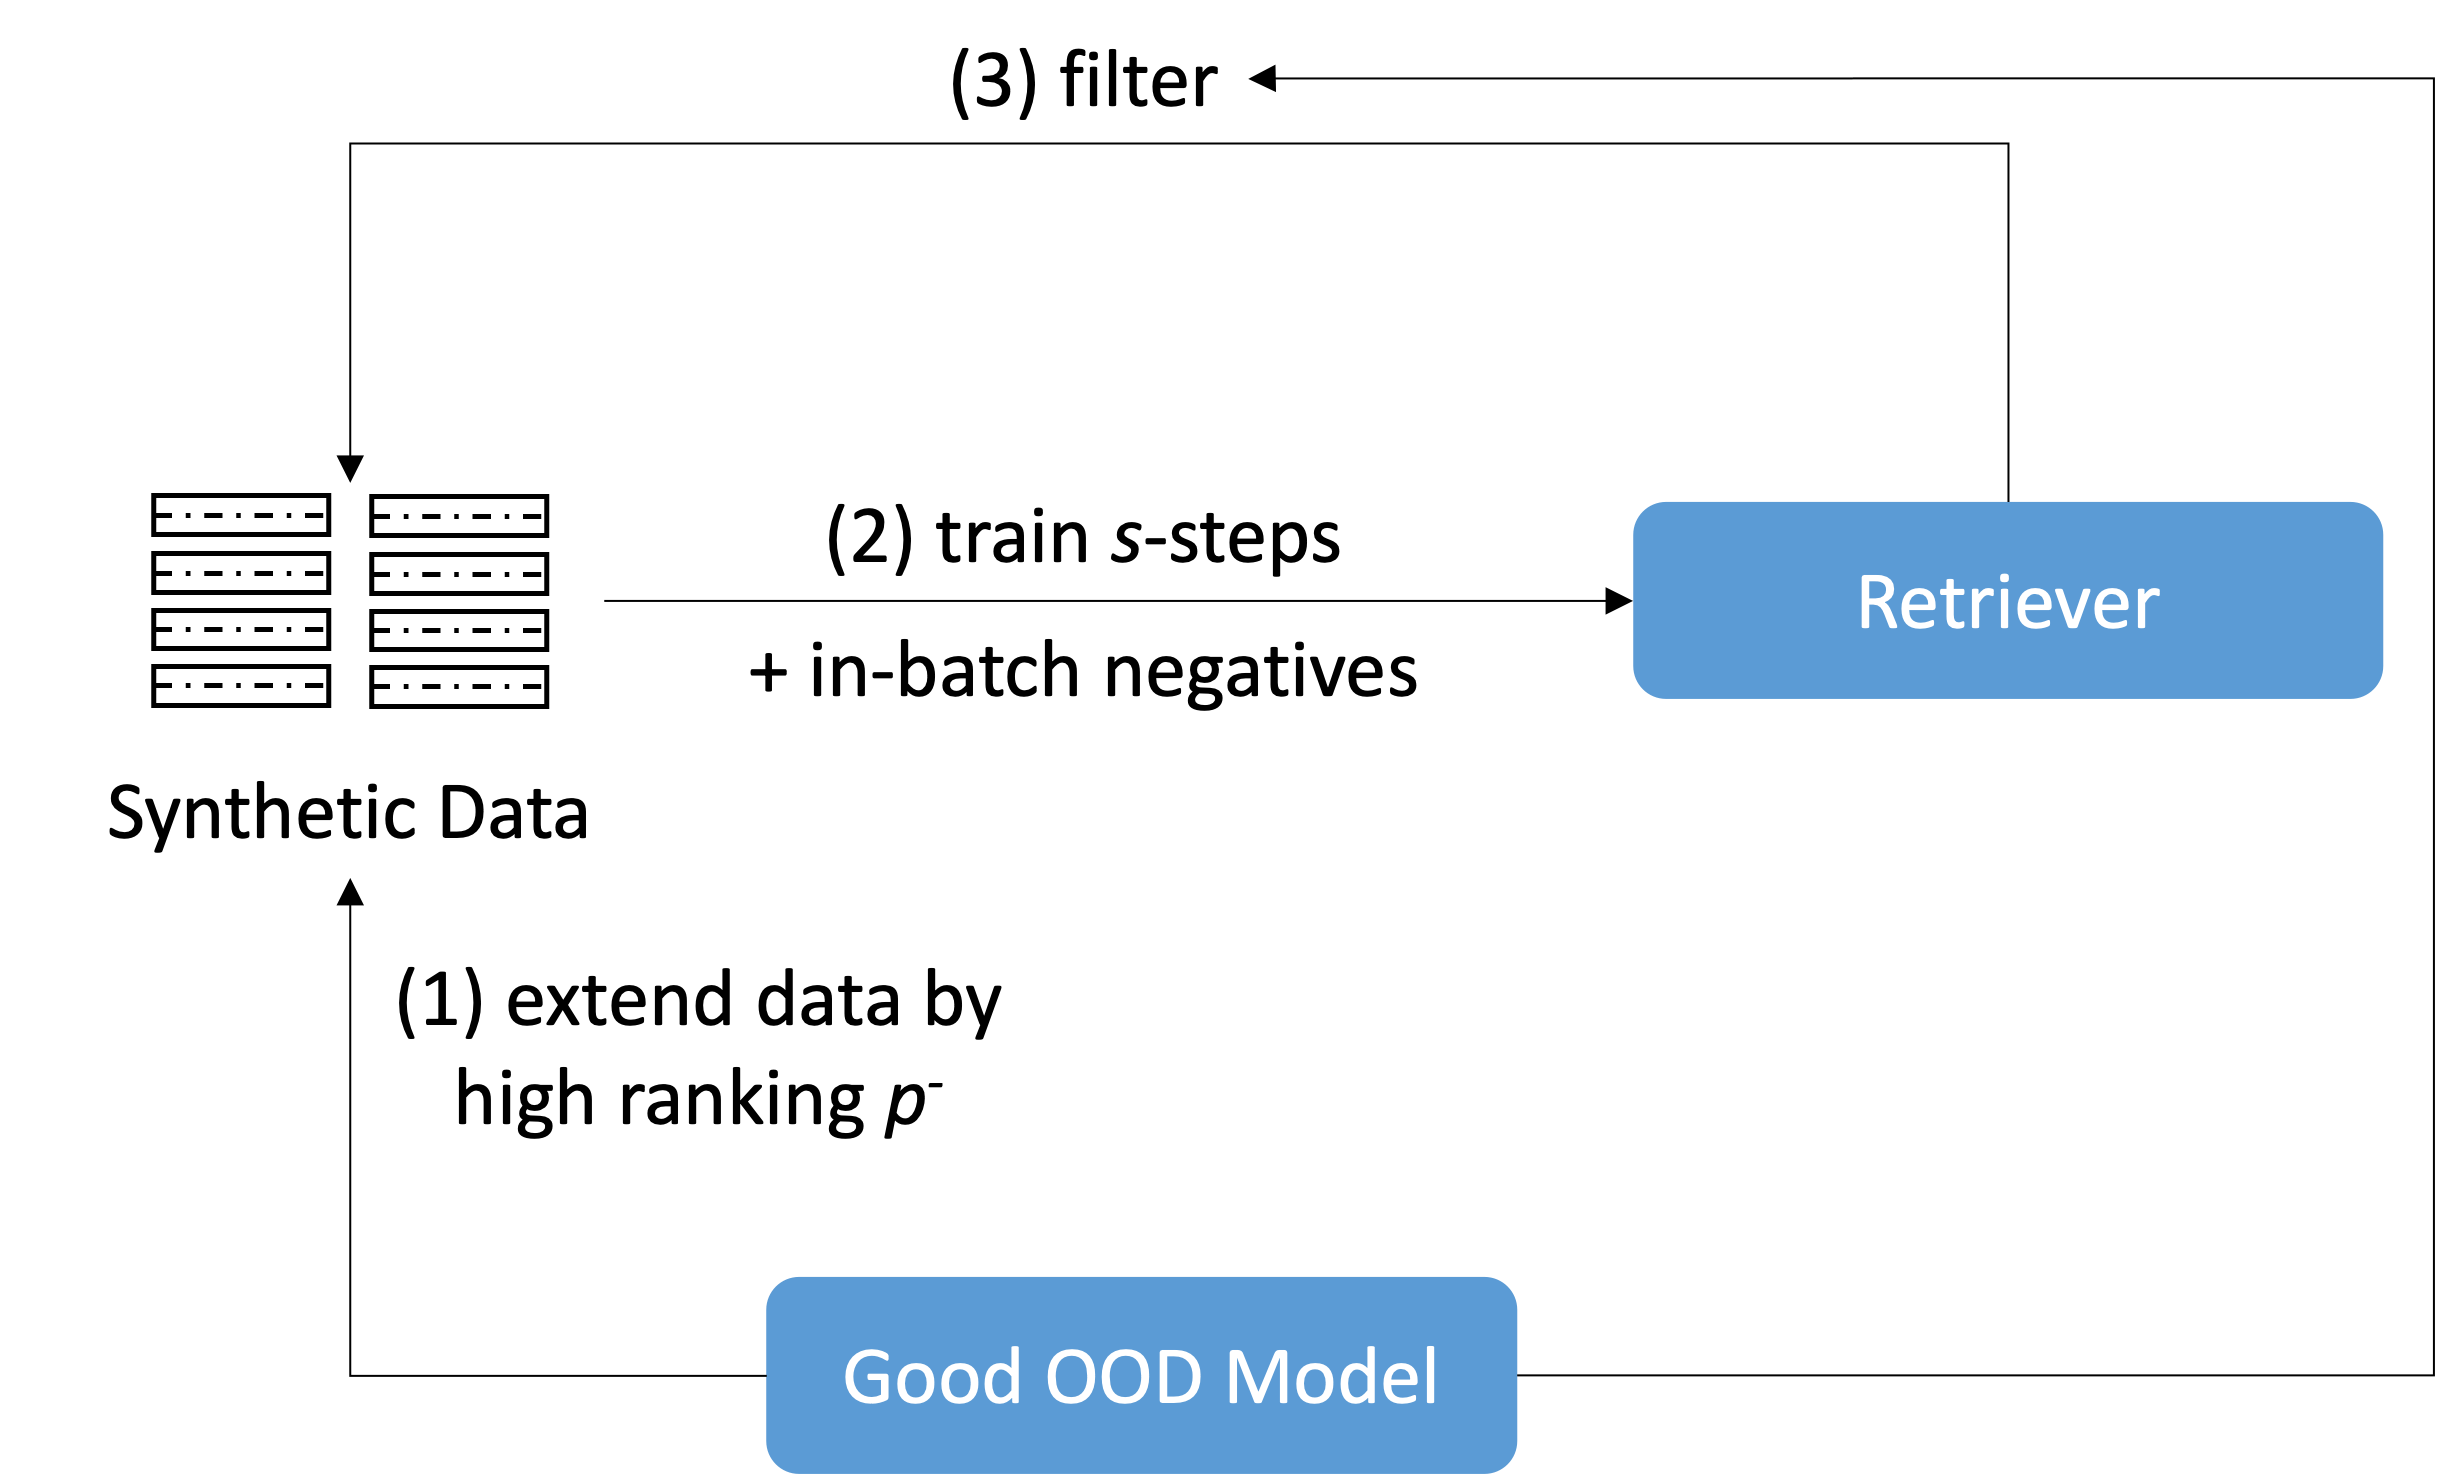
\includegraphics[width=0.8\textwidth]{Grafiken/Training.png}
    \caption{Fine-Tuning Process for Retriever}
    \label{fig:retriever-fine-tuning} 
\end{figure}




\subsection{Reader}
\label{subsec:reader}


% \section{Question Answering over PDFs}
% \label{sec:qa-over-pdfs}

% \begin{figure}
%     \centering
%     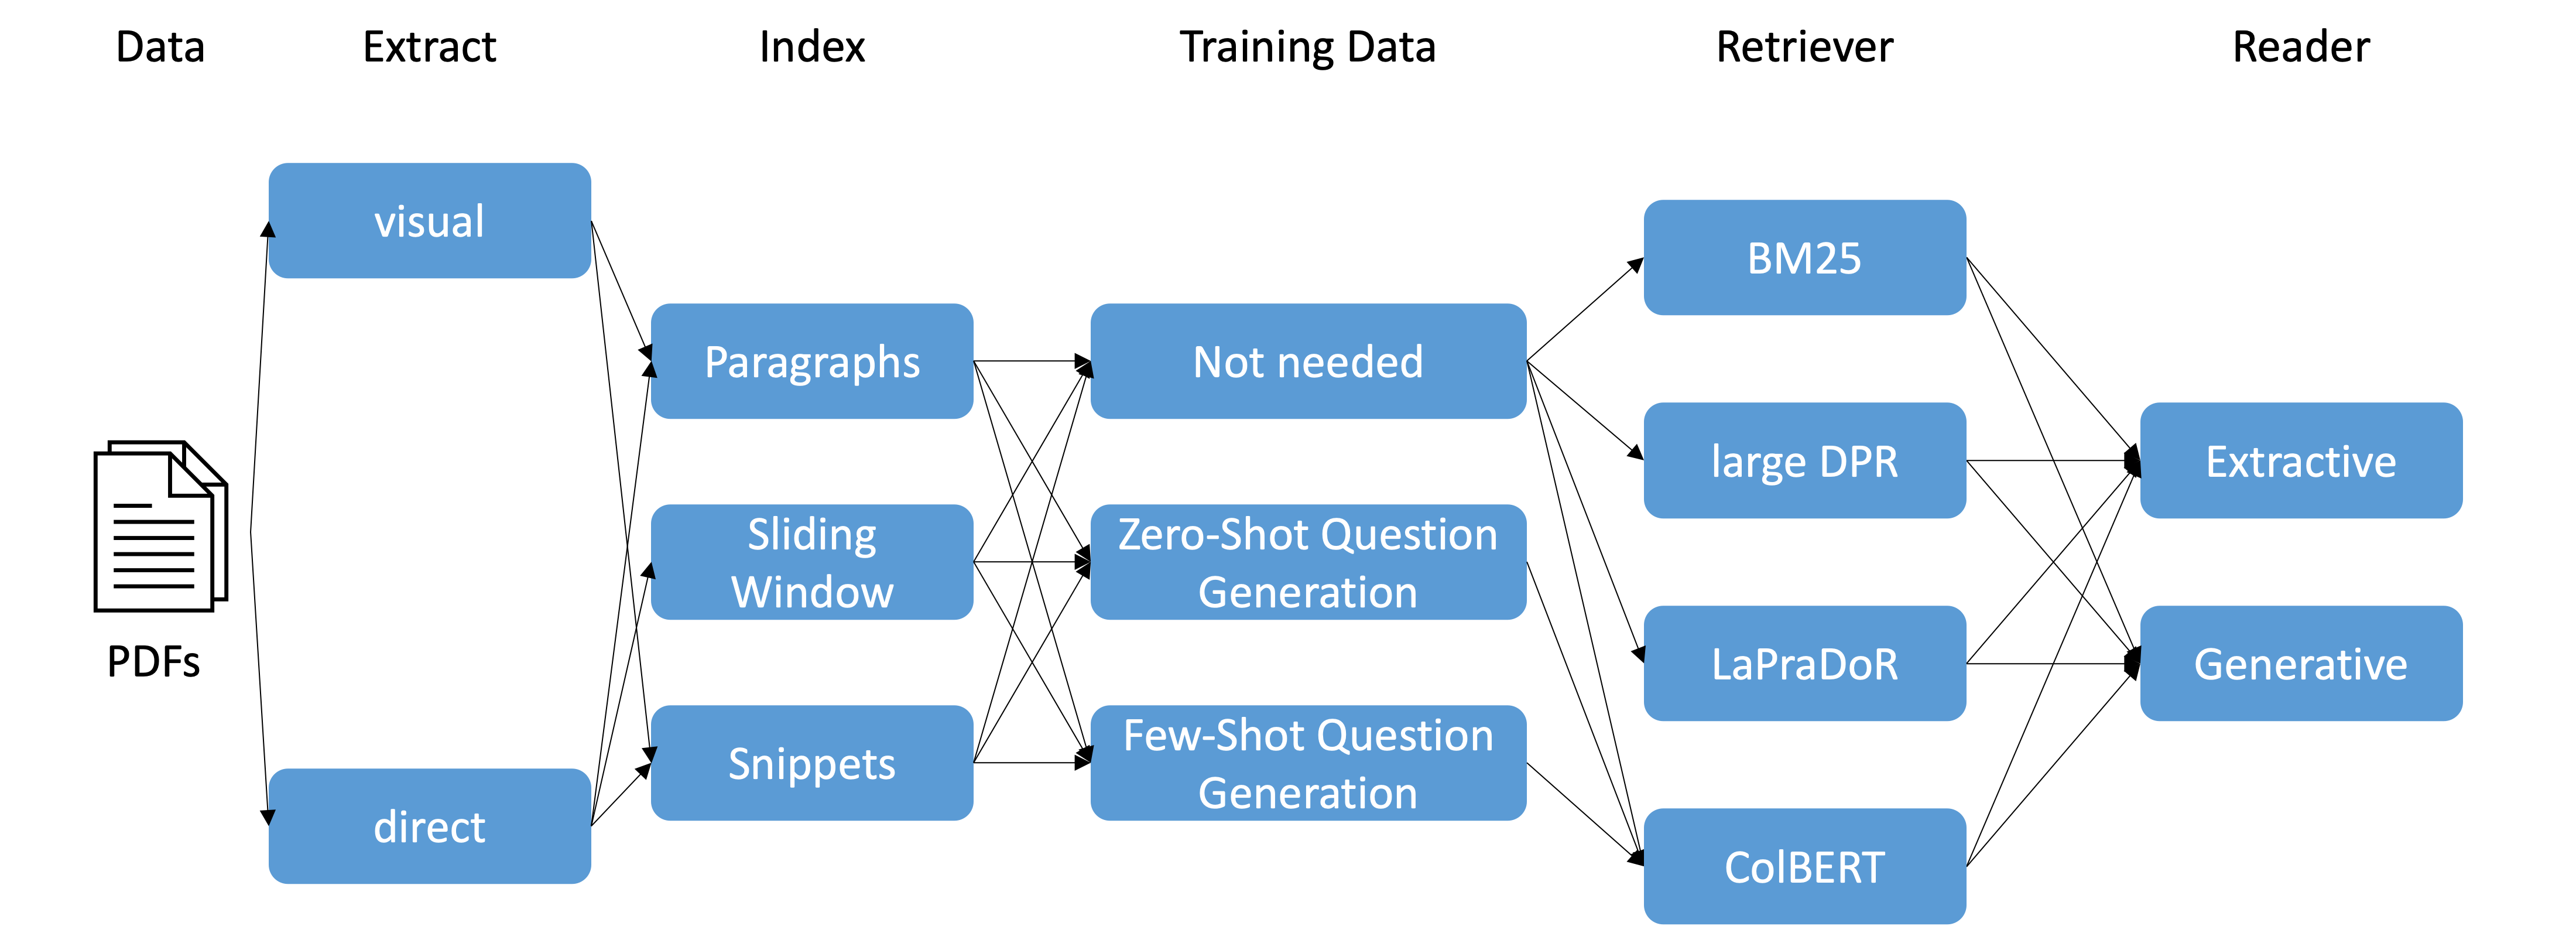
\includegraphics[width=0.8\textwidth]{Grafiken/Possible_Systems.png}
%     \caption{Possible Combinations of Modules to Create an Adapted QA-System}
%     \label{fig:qa-system-combinations}
% \end{figure}

% The possible combinations of modules to create an adapted \gls{qa}-System can be seen in Figure \ref{fig:qa-system-combinations}.


% \subsection{Extract}
% \label{subsec:extract}
% %%%%%

% \subsection{Retrieve}
% \label{subsec:retrieve}

% \textbf{Out-of-Domain Retrievers:} The easiest implementation is the out-of-domain usage of retrievers without fine-tuning and the need for generating a training dataset. Three major retrievers seem promising due to their performance on the BEIR \cite{thakur_beir_2021} out-of-domain benchmark for retrievers:

% \begin{enumerate}
%     \item \textit{BM25} is the standard Sparse Retriever based on lexical probabilistic matching between the query $q$ and passages $p$.
%     \item \textit{Large DPRs} are Dense Retrievers based on large encoders. They utilize typical dense retrieval paradigms and are a primary approach in open-source projects like \textit{Langchain} \cite{noauthor_langchain-ailangchain_nodate}.
%     \item \textit{LaPraDoR} is a hybrid retriever based on a broadly trained Representation-based Retriever, similar to (2), combined with lexical weighting (1).
% \end{enumerate}

% The \gls{laprador} utilizes the advantages of both lexical and semantic search. Given a question $q$ and a passage $p$, the semantic similarity $\text{sim}(q,d)$ is calculated using a \gls{dpr} model. In addition, the lexical similarity $\text{BM25}(q,d)$ is calculated. The final score $\text{score}(q,d)$ is computed as follows:

% \begin{equation}
%     \mathbf{score}(q, d) = \mathbf{sim}(q, d) \cdot \mathbf{BM25}(q, d)
% \end{equation}

% This approach achieves state-of-the-art performance on the BEIR benchmark without the need for fine-tuning. It serves as the ideal off-the-shelf component for the desired \gls{qa}-System.

% \noindent\textbf{Fine-Tuning Retrievers:} Fine-tuning is a challenging task in the absence of a supervised dataset, especially when dealing with a Representation-Interaction Retriever like ColBERTv2. Currently, there is no clear reference on how to fine-tune a Representation-Interaction Retriever like ColBERTv2 on synthetic data. To address this gap, this thesis proposes the approach depicted in Figure \ref{fig:retriever-fine-tuning}, which combines elements from the training processes of PROMPTAGATOR \cite{dai_promptagator_2022}, the original \gls{dpr} \cite{karpukhin_dense_2020}, and ColBERTv2 \cite{santhanam_colbertv2_2022}.

% \begin{figure}
%    \centering
%     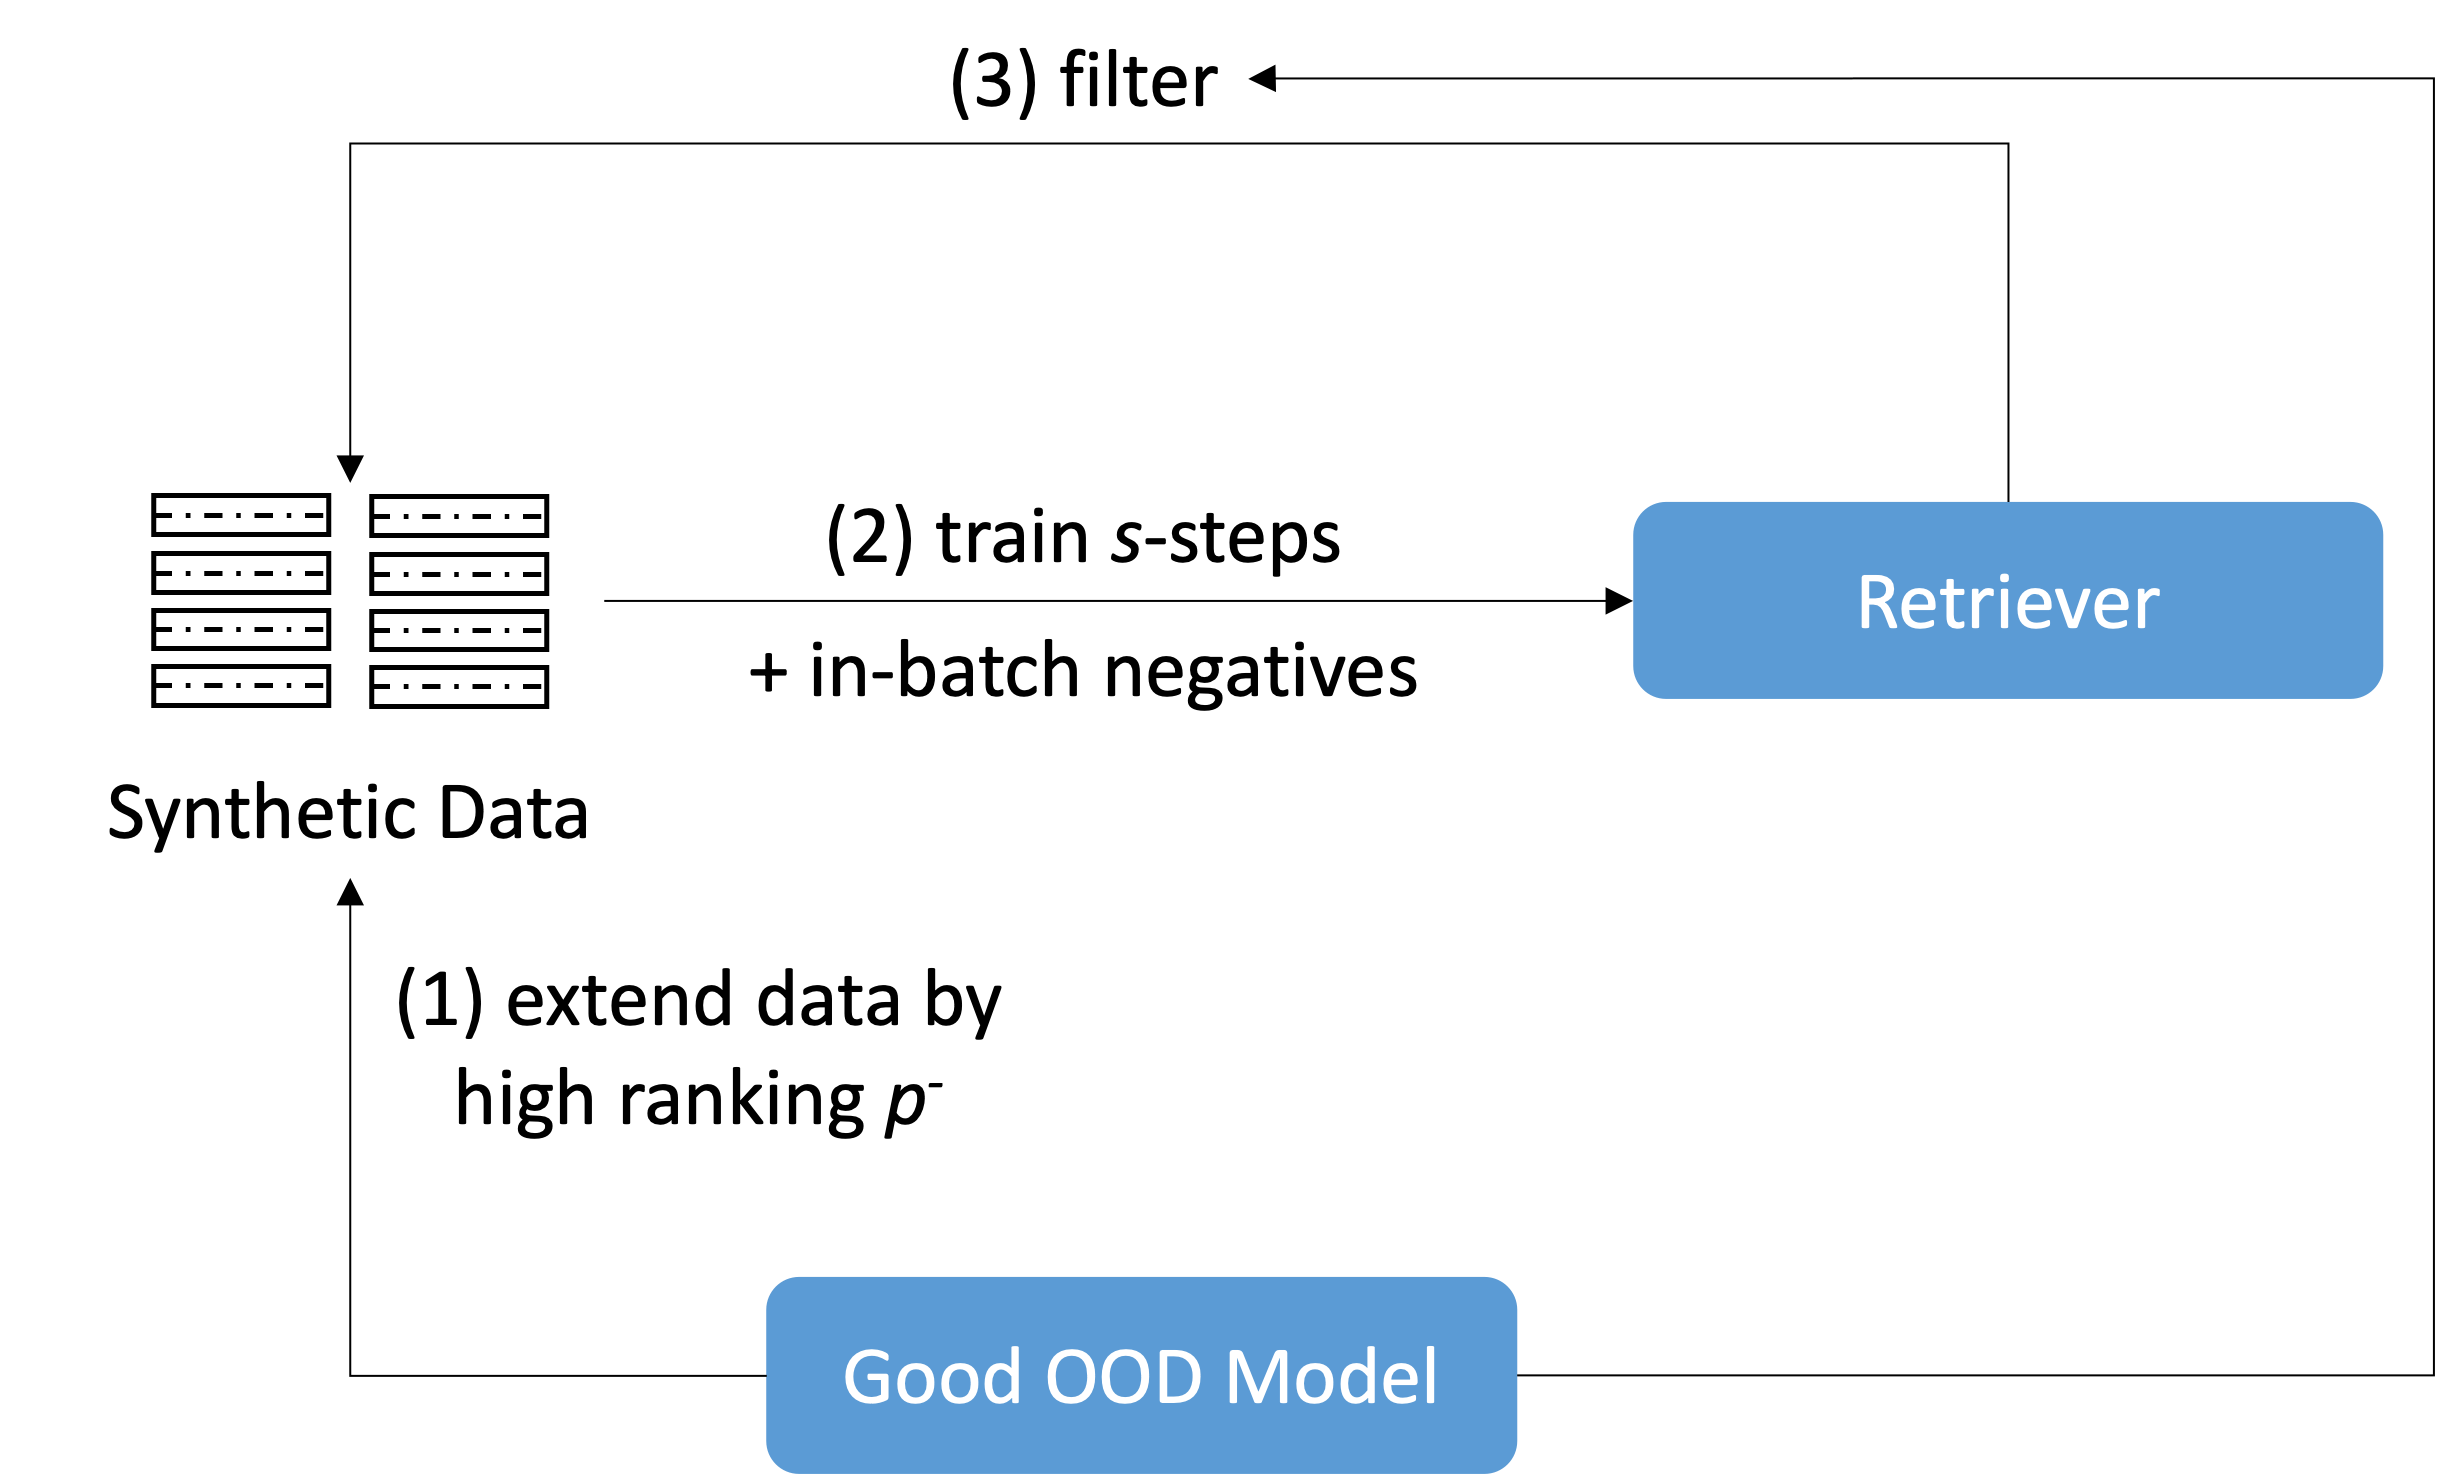
\includegraphics[width=0.8\textwidth]{Grafiken/Training.png}
%     \caption{Fine-Tuning Process for Retriever}
%     \label{fig:retriever-fine-tuning} 
% \end{figure}

% A crucial aspect of this fine-tuning approach is the utilization of an already well-performing out-of-domain retriever as a baseline. This baseline retriever can distill its knowledge into the retriever undergoing training. For example, \gls{dpr} used BM25, while ColBERTv2 employed MiniLM \cite{wang_multi-passage_2019}, a 22M-parameter Interaction-based retriever. A useful guideline for selecting the model is to consult the BEIR leaderboard.

% In the first step, the \gls{ood} model must retrieve the top $k$ passages, denoted as $p_i$, for each synthetic $(q_s,p^{+})$ pair. To generate numerous high-quality negative triples, denoted as $(q_s, p^{+}, p^{-})$, for every retrieved passage $p_i$ (where $p_i \neq p^{+}$), the triple $(q_s, p^{+}, p_i)$ is added to the training dataset.

% In the second step, the target retriever is trained for $s$ iterations. The loss function employed is the negative log likelihood, as defined in Section \ref{subsec:qa_retrieval}. During training, in-batch negatives are utilized. Let $Q$ and $P$ represent the $(B \times d)$ matrices of question and passage embeddings in a batch of size $B$. The matrix $S = Q P^{T}$ contains rows where each corresponds to a question paired with all other passages in the batch. The passages from all the other data points act as negatives for the question $q$.

% In the third step, the synthetic dataset is subjected to filtering. PROMPTAGATOR demonstrated promising results of filtering data by a network trained on the data. For this filtering process, retrieval is performed using both the newly trained model and the \gls{ood} model for a question $q_s$. If neither model retrieves the corresponding passage $p^{+}$ for the synthetic question within their top $k$, that question is removed from the dataset.

% Steps two and three are repeated once during fine-tuning.
% \subsection{Read}
% \label{subsec:read}

% \textbf{Out-of-Domain Readers:} There exists no benchmark for the application of zero-shot or \gls{ood} Readers. As Pereira et. al. \cite{pereira_visconde_2022} point out in their experimental results, the zero-shot performance of \gls{llm}s as Generative Readers is state-of-the-art and thus needs no fine-tuning and can even perform in a zero-shot setting. Luo et. al. \cite{luo_choose_2022} also pointed out, that the \gls{ood} performance of Extractive Readers is higher than the of Generative ones, when it comes to \gls{prlm}. Threfore a good \gls{ood} model choice is UnifiedQA-v2 \cite{khashabi_unifiedqa-v2_2022}, which is based on T5 \cite{raffel_exploring_2023} and was trained on 20 diverse datasets.

% \noindent\textbf{Fine-Tuning Readers:} Extractive Readers depend on datasets of the form $(q, c, a_span)$, whereas $q$ is a question, $c$ the context and $a_span$ an indication of which tokens of $c$ correspond to the desired answer. Similar for Generative Readers, which need $(q, c, a)$ datasets, whreas $a$ is just a text based answer to question $q$. The training process for the reader is easier and more straightforward as for the retriever. Given the already filtered synthetic trainings dataset, this can be used for training of the reader.

% \subsection{Orchestration}
% \label{subsec:qa_orchestration}

% Similar to \gls{r2d2}\cite{fajcik_r2-d2_2021} and LaPraDoR \cite{xu_laprador_2022} and others, an orchestration of retrievers and readers will be adopted in order to achieve highest \gls{ood} performance. This involves the following steps:

% \begin{enumerate}
%     \item \textit{Retrieval:} The $k$-top identified passages $P = \{p_1, p_2, \ldots, p_k\}$ are retrieved for a given question $q$ receive a similarity indication $\text{sim}(q,p_k)$ by the retriever. Next to this score, the BM25 score is calculated $BM25(q,p_k)$. The final score is calculated as the weighting of the similarity by BM25:     $score(q, d) = sim(q, d) \cdot BM25(q, d)$
%     \item \textit{Reader:} As for the Reader two readers will be executed at the same time: An extractive and one generative reader. Both 

% \end{enumerate}


% \section{Conversational Question Answering System}
% \label{sec:conv-qa-system}

%%%%%%%%%%%%%%%%%%%%%%%%%%%%%%%%%%%%%%%%%%%%%%%%%%%%%%%%%%%%
\newpage
%%%%%%%%%%%%%%%%%%%%%%%%%%%%%%%%%%%%%%%%%%%%%%%%%%%%%%%%%%%%

\chapter{Experimental Evaluation}
\label{chap:eval}

The previous chapter, Chapter \ref{chap:main}, layed out a holistic framework for \gls{convqa}. This chapter aims to evaluate the applicability of the established system in a real-world scenario. Section \ref{sec:data} describes the available data for the real-world scenario and delves into applied data augmentation techniques. Section \ref{sec:metrics} introduces the metrics used to evaluate the performance of the individual system components, as well as the complete \gls{convqa} system. These metrics are selected based on those used in related work. Section \ref{sec:setup} details the experimental setup, implementation specifics, and provides an implementation framework for similar use cases. Finally, Section \ref{sec:results} presents both quantitative and qualitative results from the experiments.

\section{Data}
\label{sec:data}

To evaluate the proposed system architecture and framework discussed in Chapter \ref{chap:main}, we will implement and assess its performance using the PDFs of the University of Heidelberg's examination regulations (\gls{er}). The university provides these regulations on two separate websites: one in German\footnote{\url{https://www.uni-heidelberg.de/de/studium/studienorganisation/downloadcenter/studien-und-pruefungsordnungen}} and the other in English\footnote{\url{https://www.uni-heidelberg.de/courses/download/examination_rules_regulations.html}}. It's important to note that only the German \gls{er} holds legal authority, and in cases of ambiguity between the English translation and the German original, the German \gls{er} version takes precedence.

Both websites offer structured access to the \gls{er} of nearly all faculties at the University of Heidelberg. However, it's worth mentioning that the German website is regularly updated, while the English version primarily contains outdated \gls{er}. Since there is no centralized source for accessing all English \gls{er}, the decission was made to utilize both the outdated English \gls{er} and the current German \gls{er} for this thesis. This decision aligns with the primary objective of this thesis, which is to demonstrate the \gls{poc} of the introduced framework. Obtaining the latest English \gls{er} of the University of Heidelberg is beyond the scope of this thesis.

As part of the experiments outlined in Section \ref{sec:setup}, the knowledge source of the German \gls{er} will be translated. Additional details on this process can be found in Section \ref{subsec:index}.

The two datasets (German/English) differ in their statistics. Therefore, Figure \ref{fig:er-german-stats} displays the number of documents per faculty regarding the German \gls{er}. Figure \ref{fig:er-english-stats} provides the same statistics for the English \gls{er} dataset. In general, the German dataset consists of 233 individual \gls{er}, while the English dataset contains only 151 individual \gls{er}. As observed, some faculties are overrepresented in both datasets, such as the philosophical faculty. The impact of the document distribution on the system will be discussed in Section \ref{sec:results}.

\begin{figure}
    \centering
    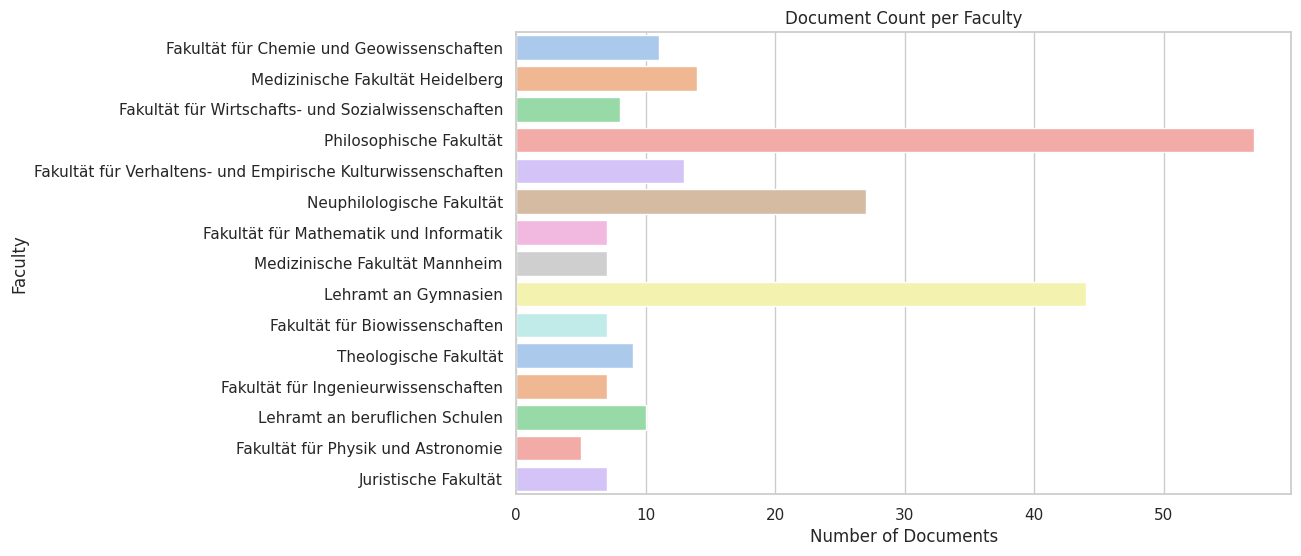
\includegraphics[width=\textwidth]{Grafiken/Statistiken/PO_german_Document Count per Faculty.png}
    \caption{Documents per Faculty of the German \gls{er} Dataset}
    \label{fig:er-german-stats}
\end{figure}

\begin{figure}
    \centering
    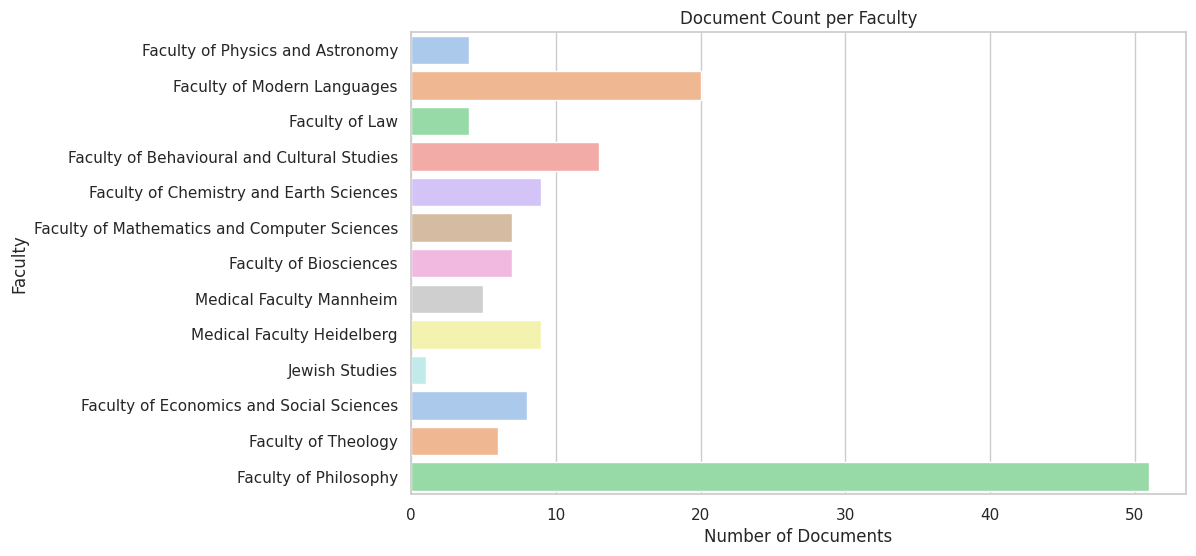
\includegraphics[width=\textwidth]{Grafiken/Statistiken/PO_english_Document Count per Faculty.png}
    \caption{Documents per Faculty of the English \gls{er} Dataset}
    \label{fig:er-english-stats}
\end{figure}

While the previous statistics described the underlying documents of the \gls{poc}, what's even more interesting are the statistics related to the final knowledge source of passages that will be used throughout the \gls{poc}. Details on how these passages have been extracted from the PDFs will be provided in Section \ref{subsec:index}. In this section, we will focus on the statistical analysis.

\begin{figure}
    \centering
    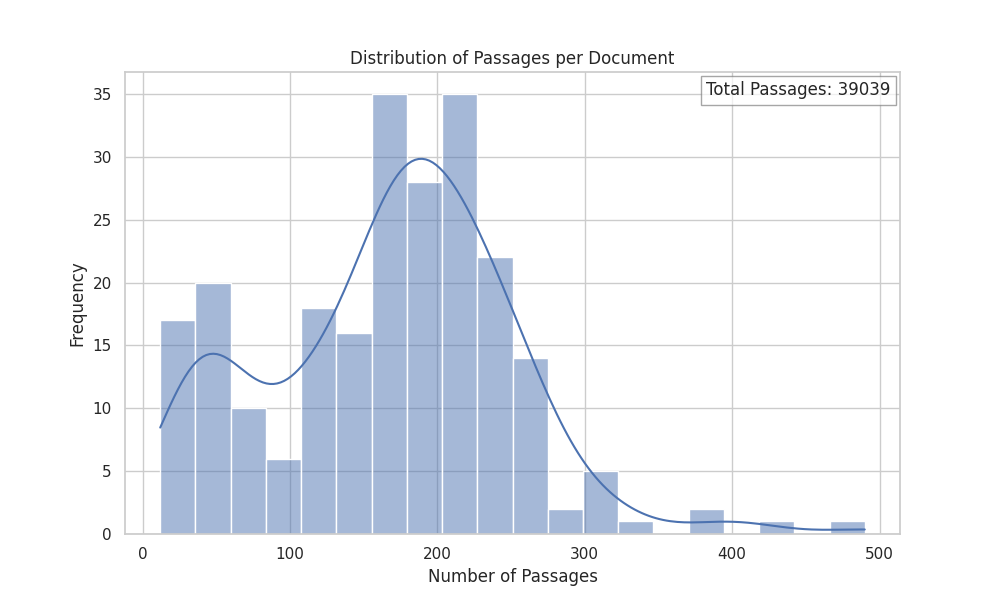
\includegraphics[width=\textwidth]{Grafiken/Statistiken/IndexGerman_Passages_Distribution.png}
    \caption{Passages per Document of the German \gls{er} Dataset}
    \label{fig:er-german-passage-document}
\end{figure}

\begin{figure}
    \centering
    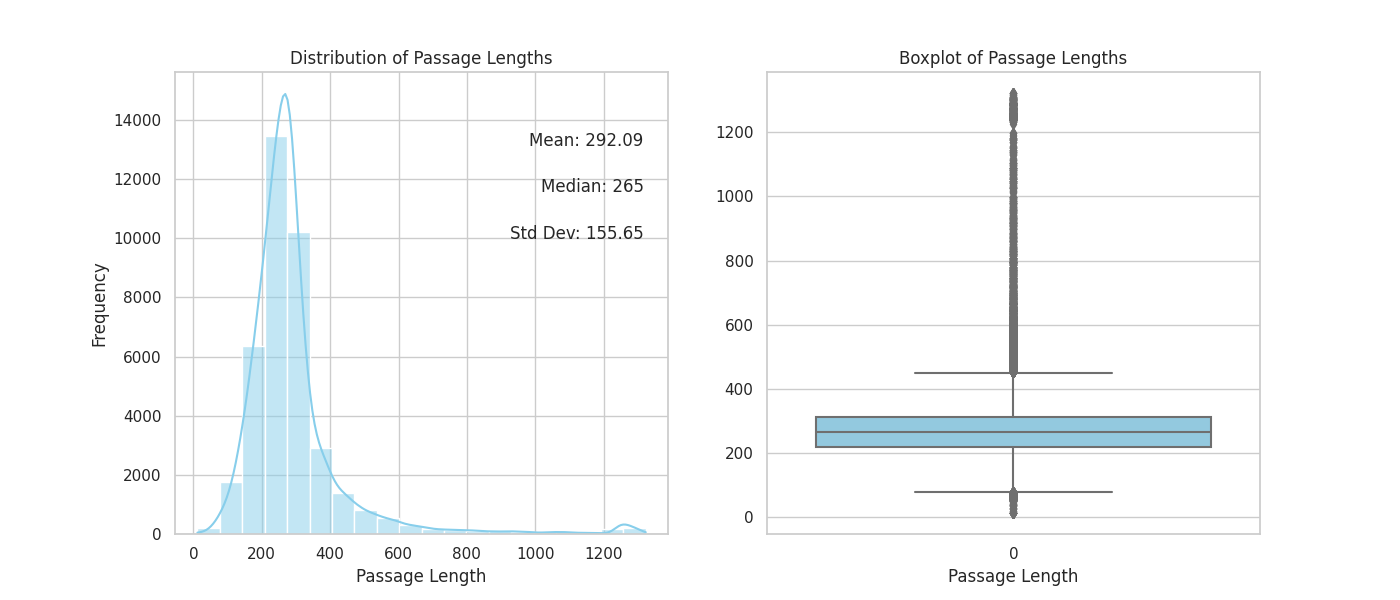
\includegraphics[width=\textwidth]{Grafiken/Statistiken/IndexGerman_Passage_Length_Statistics.png}
    \caption{Passage Length Distribution of the German \gls{er} Dataset}
    \label{fig:er-german-passage-length}
\end{figure}
Figure \ref{fig:er-german-passage-document} illustrates the distribution of passages across documents in the German dataset, offering insights into the diverse influence that documents can have on the knowledge source in terms of the number of passages. These differences in passages are mainly due to variations in the length of the examination regulations (\gls{er}). The total number of passages in the German dataset is 39,039, resulting in an average of 167.55 passages per document. In comparison, the English dataset has an average of 212.94 passages per document. The statistics for the translated dataset are similar to those of the German dataset. An apparent difference between these two datasets is that the distribution of German passages per document exhibits a slight camel-like shape with a local maximum, while the English distribution follows a clear Gaussian pattern. However, these distribution differences are not further evaluated, as we assume that they do not significantly impact the system's quality.

Figure \ref{fig:er-english-passage-document} presents the same statistics for the English dataset. As observed, the English knowledge source is smaller (31,659 vs. 38,642) than the German one, which is expected given that the English dataset contains only 151 \gls{er} compared to the 233 German \gls{er}. Still, the average number of passages per document is higher in the English dataset, as mentioned earlier. The total number of passages in the knowledge source indicates a highly closed-domain scenario. For comparison, MS MARCO \cite{bajaj2016ms}, an often-used dataset for open-domain \gls{qa}, has a knowledge source comprising 3.2 million passages, with an average length of 442 characters and passages ranging from 19 to 1,167 characters.

Figure \ref{fig:er-german-passage-length} depicts the distribution of passage lengths in the German dataset. It's evident that the majority of passages fall within the range of 200 to 350 characters. The same statistics for the English dataset are presented in Figure \ref{fig:er-english-passage-length}. As observed, they are quite similar. The shortest passage is 5 characters, as we applied a lower filter to the extracted passages. The longest passages are 1,300 characters long, also subjected to filtering. Considering statistics such as standard deviation, mean, and median, the English and German datasets do not significantly differ in terms of passage length.


\begin{figure}
    \centering
    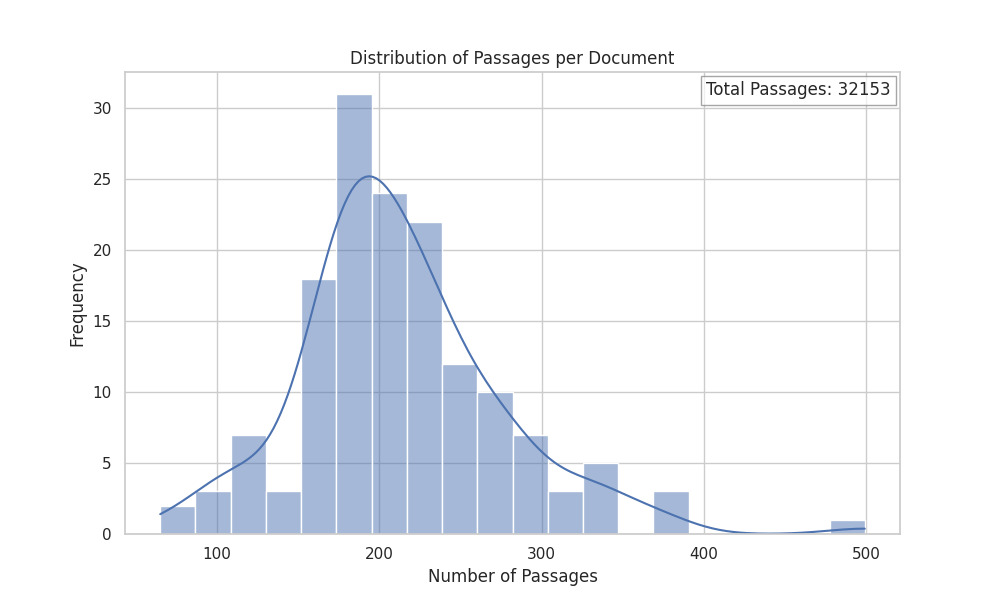
\includegraphics[width=\textwidth]{Grafiken/Statistiken/IndexEnglish_Passages_Distribution.png}
    \caption{Passages per Document of the English \gls{er} Dataset}
    \label{fig:er-english-passage-document}
\end{figure}

\begin{figure}
    \centering
    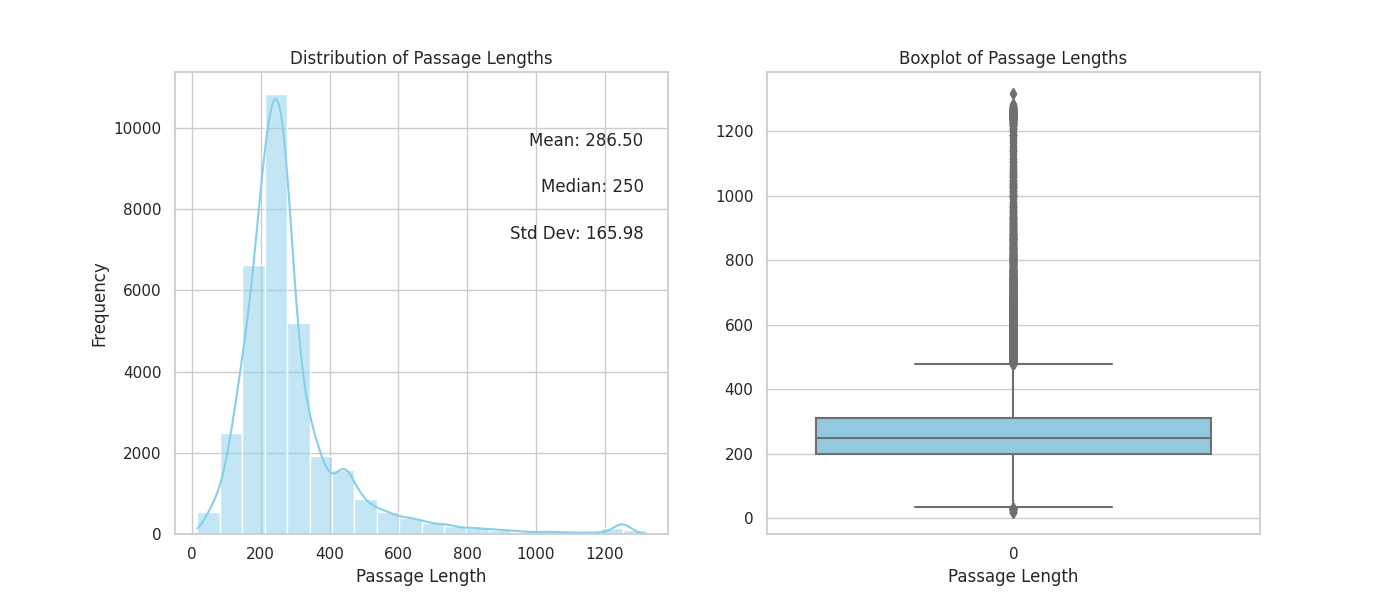
\includegraphics[width=\textwidth]{Grafiken/Statistiken/IndexEnglish_Passage_Length_Statistics.png}
    \caption{Passage Length Distribution of the English \gls{er} Dataset}
    \label{fig:er-english-passage-length}
\end{figure}


\section{Evaluation Metrics}
\label{sec:metrics}

When it comes to Evaluation Metrics, it's important to differentiate between the components or models being evaluated. For the evaluation, we will categorize the evaluation scopes as follows:

\begin{enumerate}
    \item Retrieval
    \item Reader
    \item Conversational Question Answering
\end{enumerate}

Evaluating the \gls{cqu} component is only possible with high quality human supervised datasets, therefore for the performance of the \gls{cqu} section \ref{subsec:cqu-impl} refers to previously by other works performed benchmarks of the used zero-shot models. The exact metrics and paradigms for each individual evaluation will be discussed in the following sections.

\subsection{Retrieval Evaluation}
\label{subsec:retrieval-eval}

Evaluating a Retriever largely depends on the use-case and the evaluation data available. Since the data introduced in Section \ref{sec:data} lacks a supervised dataset for $(question,\allowbreak passages)$ pairs, we will evaluate it using the synthetic dataset created, as also established in Section \ref{sec:data}. This dataset consists of $(question, passages)$ pairs, where for every question, there is an exact matching passage. Therefore, this dataset is essentially a binary task, where a passage is either the correct one or not. An alternative approach would be a graded relevance task, where each passage has a certain relevance score in relation to the question. However, for our use-case, we opted for the simpler metrics \gls{hr}@k and \gls{mrr}, instead of the Normalized Cumulative Gain (NDCG) used in benchmarks like BEIR \cite{thakur_beir_2021}. We chose these metrics because it's crucial for our system to retrieve the correct passage, and we don't have a relevance score for every passage in relation to every question.

Given a pair of $(q,\hat{p})$, where $\hat{p}$ corresponds to the correct passage and $\forall q, \exists ! \hat{p} \in P$ and a retriever model $p_\eta(p|q) = \text{Score}(q,p)$ (as defined in Definition \ref{def:retrieval}) that assigns a score to every passage $p \in P$ in relation to the question $q$ is used. We can rank all passages based on their relevance to $q$. Each passage receives a rank $r_q,p$ based on its score in relation to $q$. These passages are then ranked in descending order of $r_q,p$, and the top $k$ passages are added to the retrieved set $R_q$.

\begin{itemize}
    \item \textbf{\gls{hr}@k} This metric calculates the proportion of questions for which the correct passage is retrieved within the top $k$ retrieved passages.
    \begin{equation}
        \text{HR@k} = \frac{1}{|Q|} \sum_{q \in Q} 
        \begin{cases}
            1 & \text{if } \hat{p}_q \in R_{q,k} \\
            0 & \text{otherwise}
        \end{cases}
        \in [0,1]
    \end{equation}
    The \gls{hr}@k is a straightforward metric that provides a value between 0 and 1, with a higher value indicating the percentage of cases where the correct passage was retrieved within the top $k$ passages.
    \item \textbf{\gls{mrr}} This metric computes the mean reciprocal rank of the correct passage. It is similar to \gls{hr}@k but considers the position of the correct passage $\hat{p}q$ within the ranking $R_q$.
    \begin{equation}
        \text{MRR} = \frac{1}{|Q|} \sum_{q \in Q} \frac{1}{r_{q,\hat{p}_q}} \in [0,1]
    \end{equation}
    In an ideal system, the \gls{mrr} would be 1, indicating that the correct passage is always retrieved in the first position ($r_{q,\hat{p}} = 1$) for all $q \in Q$.
\end{itemize}

\subsection{Reader Evaluation}
\label{subsec:answer-generation-eval}

Evaluating the task of answer generation, particularly the \gls{mrc} aspect of the reader component, presents challenges similar to those discussed for the retrieval task evaluation in Section \ref{subsec:retrieval-eval}. For automatic and manual evaluation, we will utilize the synthetic dataset generated in Section \ref{sec:data}. This dataset comprises triples of $(\text{question}, \text{passages}, \text{answer})$, where \textit{answer} refers to a gold answer that has been syntactically generated.

In the context of a triple $(q, \hat{p}, \hat{a})$, where $\hat{p}$ corresponds to the correct passage and $\hat{a}$ corresponds to the correct answer in relation to a question $q$, we employ a reader model $p_\theta(a' \, | \, q, \hat{p}) := \hat{a}$ (as defined in Definition \ref{def:generation}) to predict the answer $\hat{a}$ given the question $q$ and the passage $\hat{p}$. The predicted answer $a'$ is then evaluated using the following metrics:

\begin{itemize}
    \item \textbf{BLUE-1:} This precision-oriented metric compares the occurrence of unigrams (words $w \in \hat{a}$) in the predicted answer $a'$ and the gold answer $\hat{a}$.
    \begin{equation}
        \text{BLUE-1} = \frac{\sum_{w \in a'} \min(\text{count}_{a'}(w), \text{count}_{\hat{a}}(w))}{\sum_{w \in a'} \text{count}_{a'}(w)} \in [0,1]
    \end{equation}
    Here, $\text{count}_{a'}(w)$ represents the number of occurrences of the word $w$ in the predicted answer $a'$. \gls{bleu} is particularly useful for evaluating extractive questions \cite{papineni_bleu_2002}.

    \item \textbf{ROUGE-L:} This recall-oriented metric, especially \gls{rogue}-L, compares the longest common subsequence ($LCS$) between the predicted answer $a'$ and the gold answer $\hat{a}$.
    \begin{align}
        R_{LCS} &= \frac{LCS(\hat{a}, a')}{|\hat{a}|} \\
        P_{LCS} &= \frac{LCS(\hat{a}, a')}{|a'|} \\
        \text{ROUGE-L} &= \frac{(1+\beta^2)R_{LCS}P_{LCS}}{R_{LCS}+\beta^2P_{LCS}} \in [0,1]
    \end{align}
    Here, $\beta$ is a parameter to balance between precision and recall. Rouge operates similarly to \gls{bleu} but focuses on lexical matching \cite{lin_rouge_2004}.

    \item \textbf{F1-BERTscore}: BERTscore is a \gls{s2s}-model-based evaluation metric for comparing two text fragments: $x$, which is the reference, and $\hat{x}$, which is the prediction. In this context, the predicted answer $a'$ is compared to the gold answer $\hat{a}$. Essentially, the score between two tokens, $a'_i$ and $\hat{a}_i$, is calculated as the inner product of their respective BERT embeddings: $\text{BERT}(a'_i)^T\text{BERT}(\hat{a}_i)$. For simplicity, we'll use the  $\text{BERT}(a'_i) \rightarrow a'_i$ in the following equations. The final scores of F1-BERTscore are weighted by the inverse document frequency (idf) of each word-piece token:

    \begin{align}
        P_{BERT} &= \frac{\sum_{a'_j\in a'} \text{idf}(a') \max_{\hat{a}_i \in \hat{a}} (\hat{a}_i^T a'_j)}{\sum_{a'_j\in a'} \text{idf}(a')} \\
        R_{BERT} &= \frac{\sum_{\hat{a}_i \in \hat{a}} \text{idf}(\hat{a}_i) \max_{a'_j \in a'} (\hat{a}_i^T a'_j)}{\sum_{\hat{a}_i \in \hat{a}} \text{idf}(\hat{a}_i)} \\
        F1_{BERT} &= \frac{2P_{BERT}R_{BERT}}{P_{BERT}+R_{BERT}}
    \end{align}
    
    The advantage of F1-BERTscore lies in its reliance on semantic matching between the gold answer $\hat{a}$ and the predicted answer $a'$ rather than mere lexical matching \cite{zhang_bertscore_2020}.
    

    \item \textbf{Accuracy} This metric calculates the proportion of questions for which the predicted answer $a'$ matches the gold answer $\hat{a}$. 
    \begin{equation}
        \text{Accuracy} = \frac{1}{|Q|} \sum_{q \in Q} 
        \begin{cases}
            1 & \text{if } a' = \hat{a} \\
            0 & \text{otherwise}
        \end{cases}
        \in [0,1]
    \end{equation}
    This metric is useful for evaluating question, answer realtions, where there is only one correct answer. In order to define if an answer is correct or not, the following approaches will be used:
    \begin{itemize}
        \item \textbf{LLM-based:} A \gls{llm} can be prompted to determine a binary value (0 or 1) indicating whether the underlying message of $a'$ and $\hat{a}$ matches. The prompt used is based on the work of \cite{kamalloo_evaluating_2023}:
        \begin{quote}
            \texttt{Question:} q \\
            \texttt{Gold Answer:} $\hat{a}$ \\
            \texttt{Predicted Answer:} a' \\
            \texttt{Is the predicted answer correct?} Yes/No
        \end{quote}
        This appraoch is especially useful for evaluating generative questions, as it allows for semantic matching.
        \item \textbf{Human-based:} A human evaluator is asked to assign a binary value of 0 or 1 to indicate whether there is a match in the underlying message of $a'$ and $\hat{a}$. 1 if the answer $a'$ covers the information from $\hat{a}$, and 0 if it does not. The evaluator is provided with the question $q$, the important passage $\hat{p}$, the gold answer $\hat{a}$, and the generated answer $a'$. This approach is particularly useful for evaluating generative questions and closely resembles real-world applications. For this thesis two evaluaters will receive the same 100 randomly sampled answers and will be asked to assign a binary value to each answer. The inter-rater agreement will be calculated using Cohen's Kappa \cite{cohen_coefficient_1960}. 
    \end{itemize}
\end{itemize}
    
\subsection{Conversational Question Answering Evaluation}
\label{subsec:convqa-eval}

The most challenging aspect of evaluation within the context of the system developed here is assessing \gls{convqa} as a holistic system. Instead of presenting evaluation metrics in this section, we will explore the approaches for evaluating \gls{convqa}, and as final metrics, we will use those introduced in Sections \ref{subsec:answer-generation-eval} and \ref{subsec:retrieval-eval}. Generally, two approaches can be considered: 

The first approach, known as \textbf{Manual Human Evaluation (\gls{mahueval})}, operates as follows:

\begin{enumerate}
    \item A human evaluator initiates a conversation with a question, either based on their own intuition or using provided questions from the supervised dataset. Evaluators are encouraged to pose context-dependent questions.
    \item The evaluator continues the conversation, asking follow-up questions or engaging in a general discussion with the \gls{convqa}-System for 8-10 turns.
    \item After the conversation, the evaluator has access to the retrieved passages $p$ for each turn and all other passages $P$ in the index. The evaluator assesses the answer provided by the system and the relevance of the retrieved passages $p$. They are required to provide the following information:
        \begin{itemize}
            \item \textit{Question Intent:} The evaluator specifies the intent of the question, which can be categorized as either \textit{extractive}, \textit{abstractive}, or \textit{boolean}.
            \item \textit{Answer:} The evaluator assigns a binary value (0 or 1) to the system's answer. A score of 1 indicates a correct answer, while 0 represents an incorrect answer.
            \item \textit{Passage:} The evaluator assigns a binary value (0 or 1) to the relevance of the retrieved passages $p$. A score of 1 indicates that the passages are relevant for generating the correct answer, while 0 indicates irrelevance.
        \end{itemize}
    \item Based on the provided scores, metrics for the retriever and reader will be calculated for each turn, the entire conversation history, and the entire dataset. \textit{Accuracy} will be computed for answers, and \textit{HR@k} will be computed for passages. All results will be grouped by turn, enabling deeper insights into the performance and errors of the system.
\end{enumerate}

To mitigate bias, human manual evaluations are conducted by two different evaluators. Each evaluator conducts 10 conversations with the system in the first round. In the second round, the evaluators initiate conversations with the first question from the 10 conversations of the other evaluator. This results in a total of 40 conversations and, ideally, 20 overlapping conversations that can be used to calculate inter-rater agreement \cite{cohen_coefficient_1960}.

The second approach, \textbf{\gls{auev}}, operates as follows. In this approach, a synthetic dataset is provided, consisting of lists of triples $(q, \hat{p}, \hat{a})$, where each triple corresponds to one turn, and a list represents a conversation history $h \in H$:

\begin{enumerate}
    \item Initially, the system is presented with the first question $q_1$ from the conversation history. The response $a'_1$ is evaluated using the \textit{F1-BERTscore} in comparison to the gold answer $\hat{a}$ of the history $h$. This score is computed for each turn, assessing the system's response against the gold answer for that turn.
    \item Subsequently, to mitigate the impact of an incorrect system response on the ongoing conversation, the following question (e.g., $q_2$) is augmented with the gold answer $\hat{a}_1$. This augmentation helps address missing information or coreference problems caused by an erroneous response. This method, originally introduced by Li et al. \cite{li_ditch_2022}, improves the automatic evaluation of \gls{convqa} systems. The model used to resolve the relationship between the gold answer and the question is the standard CQU model. Additionally, within the \gls{convqa} history, the answer $a'_1$ is replaced by the gold answer $\hat{a}_1$ for the CQU unit.
    \item After enhancing the question, the system is tasked with generating a response $a'_2$ to the augmented question $q'_2$. Once again, the response $a'_2$ is evaluated using the \textit{F1-BERTscore} against the gold answer $\hat{a}_2$ from the history $h$.
    \item Steps (2) and (3) are repeated until the end of the conversation history $h$.
    \item All scores will be groupable by turn depth, enabling deeper insights into the performance and errors of the system.
\end{enumerate}

Both \gls{mahueval} and \gls{auev} will be employed to evaluate the \gls{convqa} system, and the results will be reported separately.

\section{Experimental Setup and Implementation}
\label{sec:setup}

This section outlines the experimental setup and provides details on the implementation of the System Architecture and Framework introduced in Chapter \ref{chap:main}. First and foremost, we apply the theoretically outlined model ($M$) to create an implementation decision map. Figure \ref{fig:extract-pipeline-implementation-grid} illustrates a decision tree showcasing the possible implementations of the \textit{Extract} pipeline. Figure \ref{fig:all-components-conrag-grid} displays the main components, namely the \textit{Retriever}, \textit{Reader}, and \textit{\gls{cqu}}, in a similar decision matrix, where each column represents a decision to be made during implementation. Opting not to make a decision is also a valid choice. Developing an implementation can then be easily achieved using a decision tree, as shown in Figure \ref{fig:example-implementation-tree}. For the implementation and benchmarking, ressources of the BwUniCluster\footnote{\url{https://wiki.bwhpc.de/e/BwUniCluster2.0}} have been used.

\begin{figure}
    \centering
    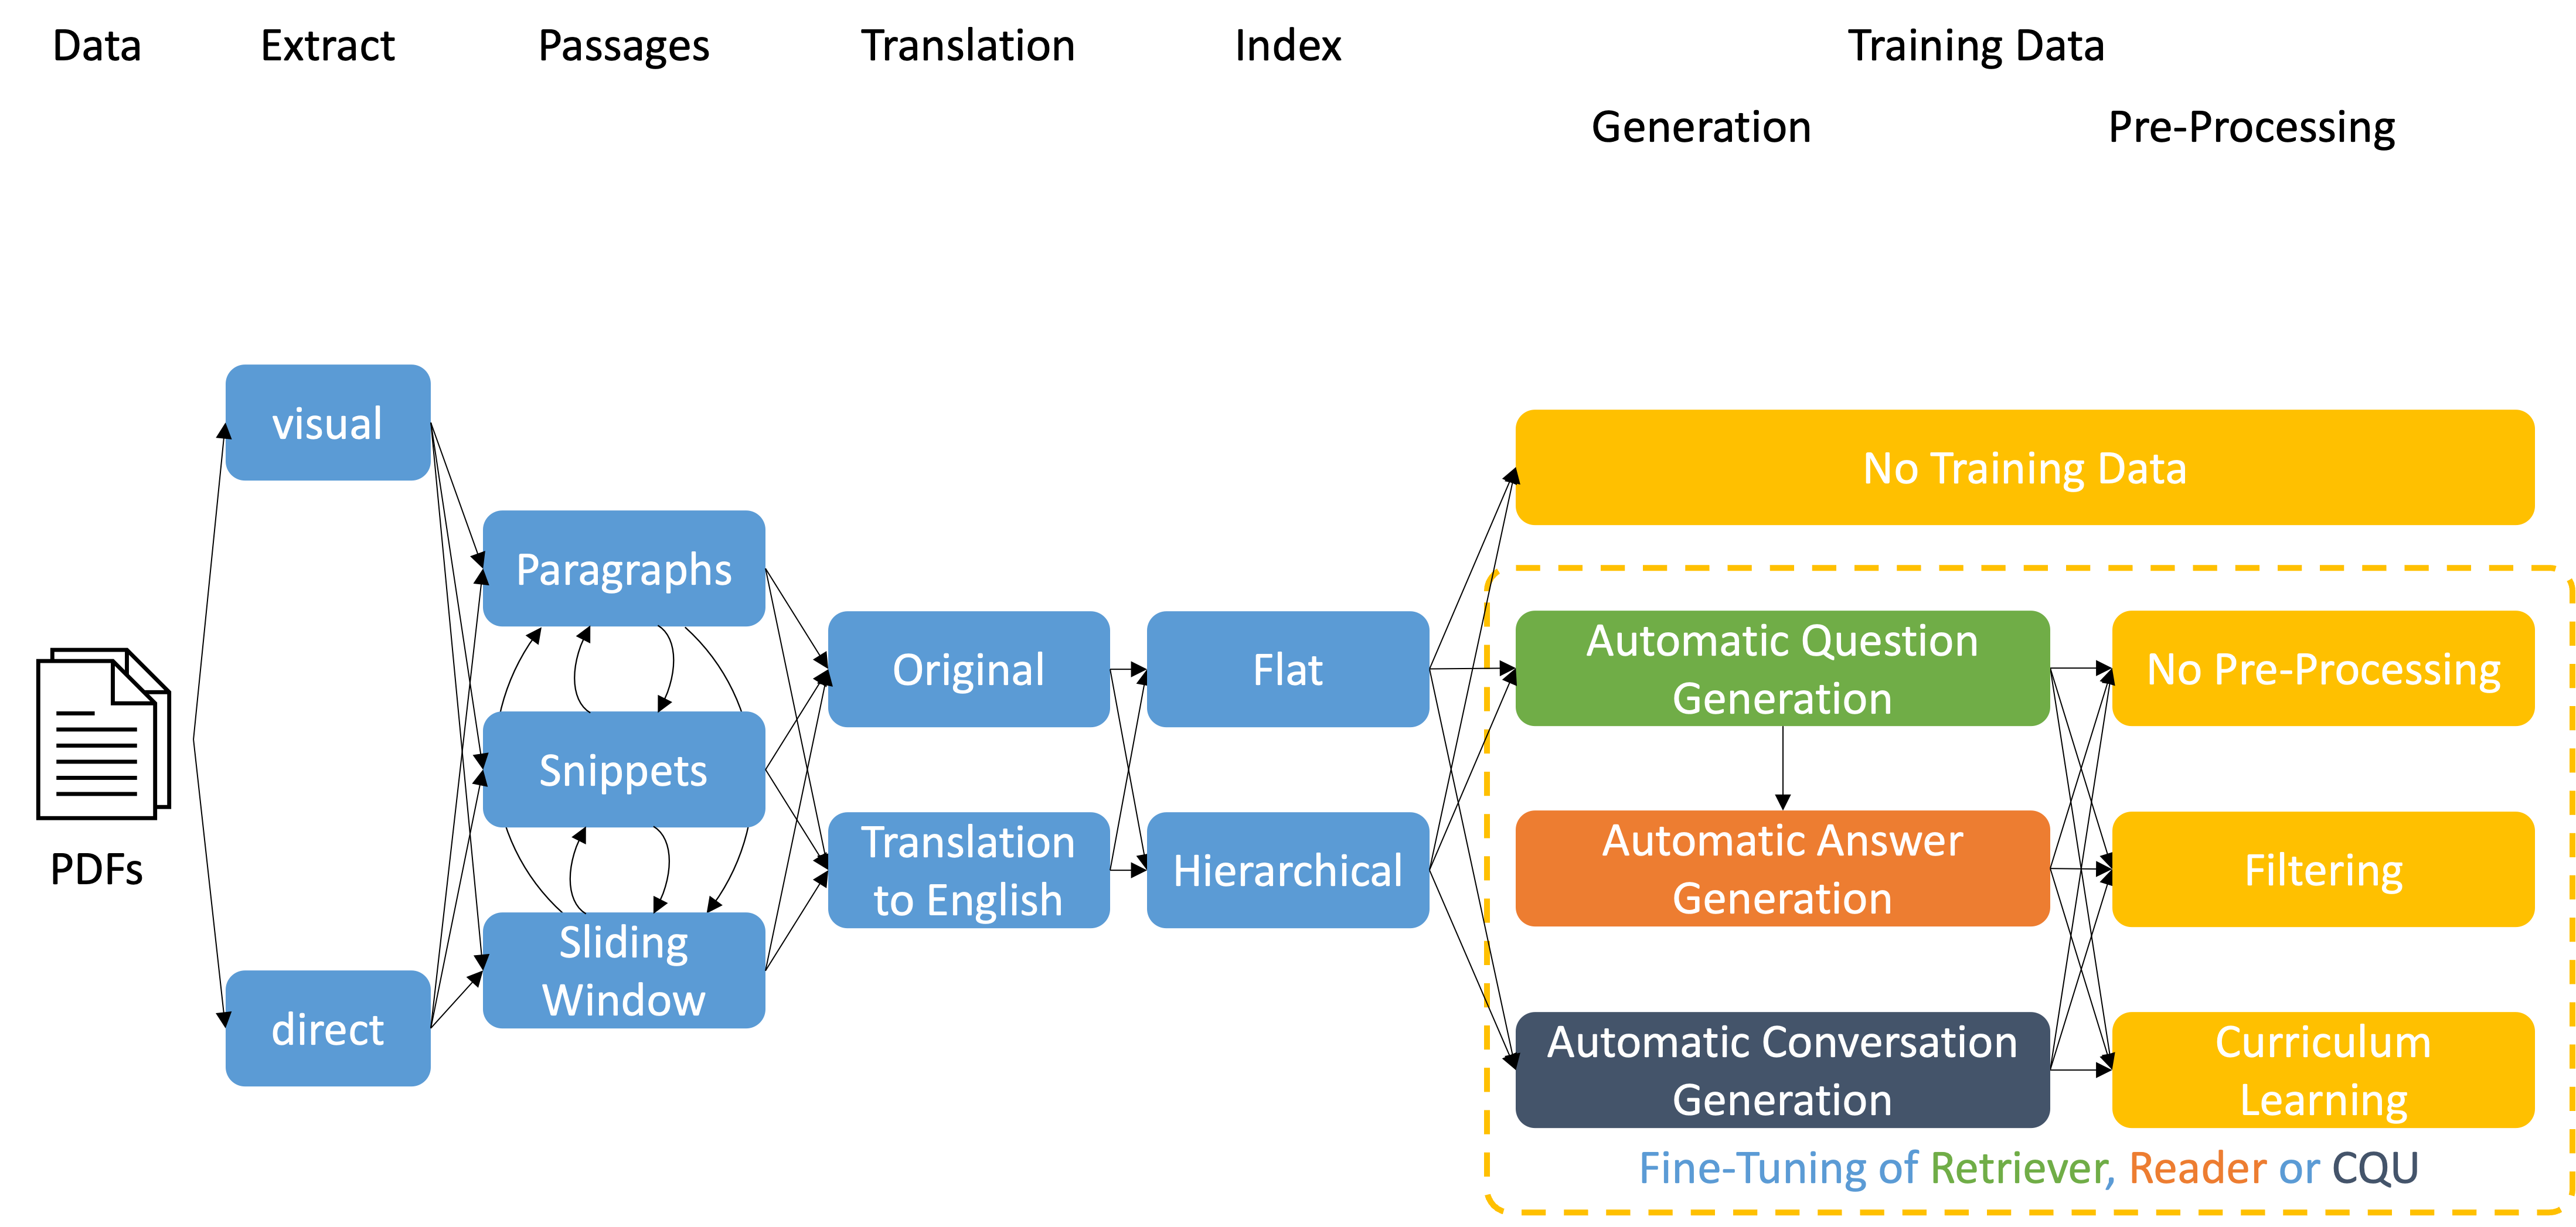
\includegraphics[width=\textwidth]{Grafiken/extract_pipeline.png}
    \caption{Possible Implementations of the Extract Pipeline}
    \label{fig:extract-pipeline-implementation-grid}
\end{figure}

\begin{figure}
    \centering
    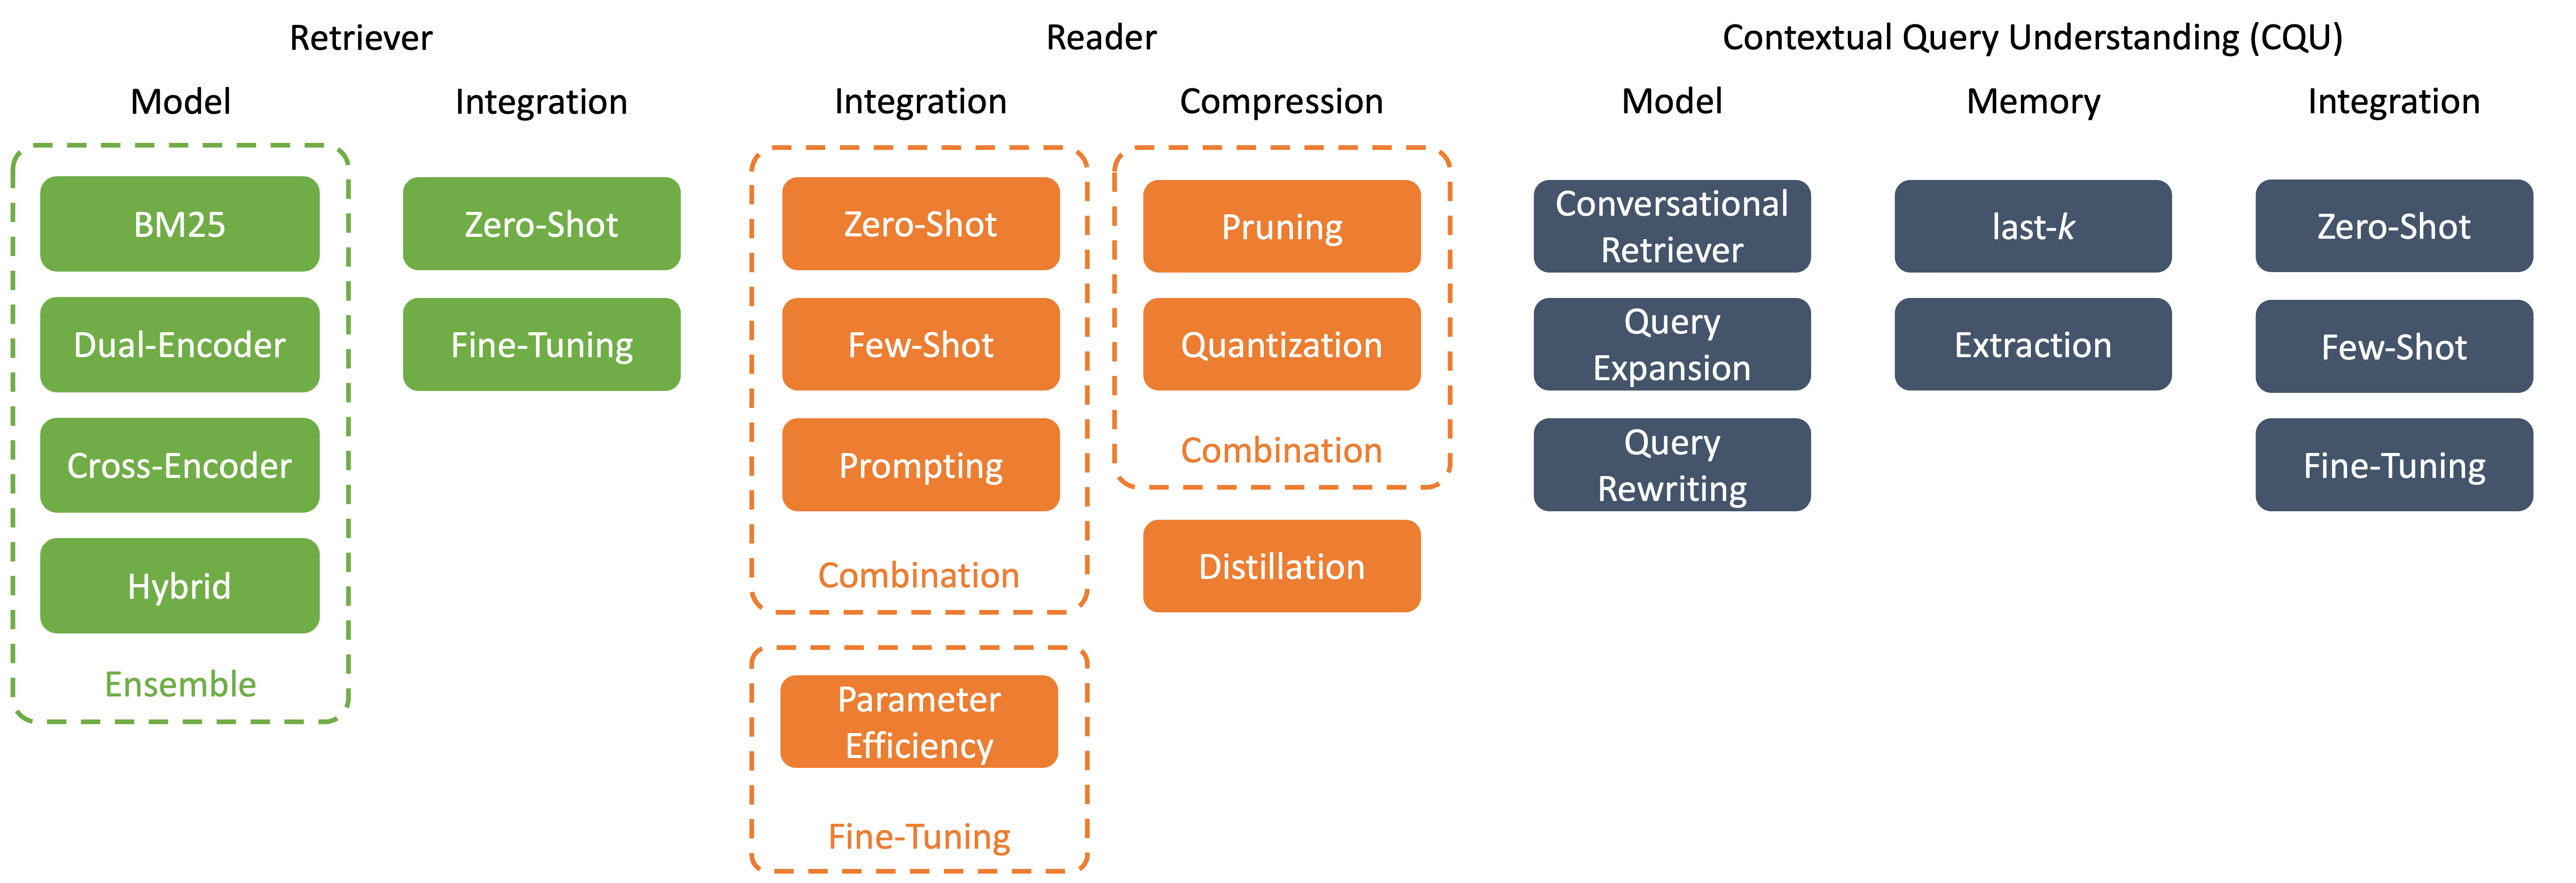
\includegraphics[width=\textwidth]{Grafiken/all_components_conrag.png}
    \caption{All Components of the System Architecture}
    \label{fig:all-components-conrag-grid}
\end{figure}

\subsection{Extraction}
\label{subsec:index}

Figure \ref{fig:extract-pipeline-implementation} illustrates the extraction pipeline implemented for this thesis' \gls{poc}, resulting in the creation of the \textit{document model} of the passages forming the knowledge source. This pipeline comprises the following steps:

\begin{figure}
    \centering
    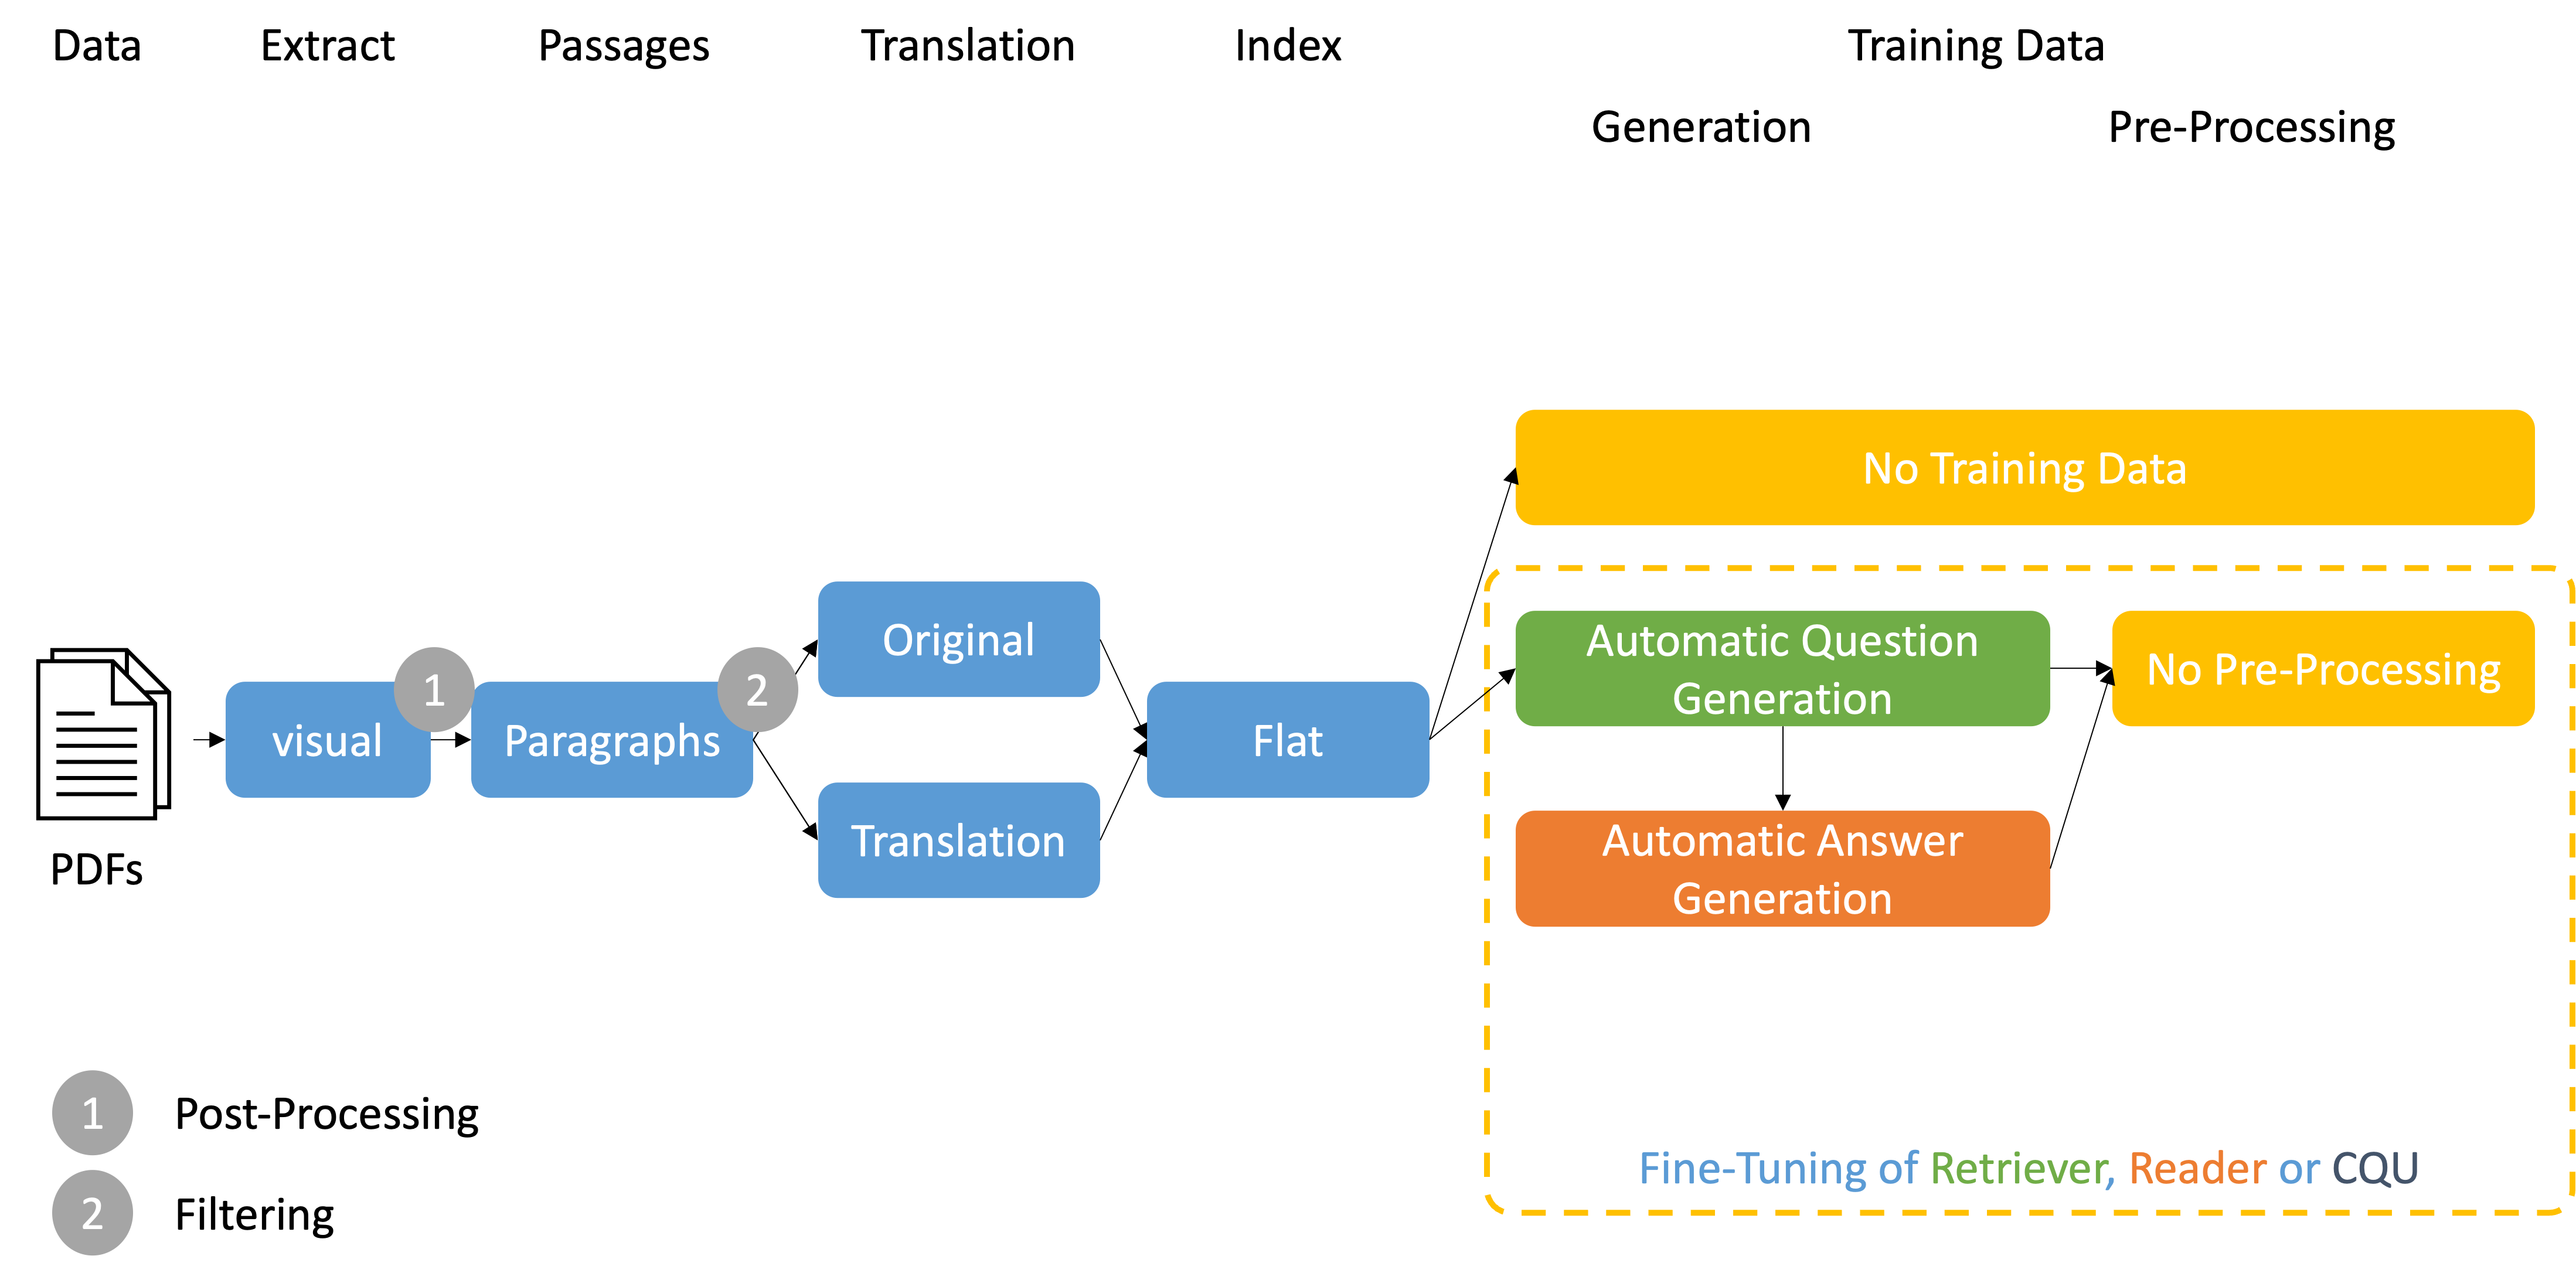
\includegraphics[width=\textwidth]{Grafiken/Evaluation/extract_implemented.png}
    \caption{Implemented Extraction Pipeline}
    \label{fig:extract-pipeline-implementation}
\end{figure}

\begin{enumerate}
    \item \textit{Extract:} Visual extraction using the Google Cloud Vision API for PDF OCR\footnote{\url{https://cloud.google.com/vision/docs/pdf}}, followed by post-processing.
    \item \textit{Passages:} Extraction of paragraphs using the NLTK tokenizer-based Text Splitter by Langchain\footnote{\url{https://python.langchain.com/docs/modules/data\_connection/document\_transformers/text\_splitters/split\_by\_token\#nltk}}, followed by filtering.
    \item \textit{Translation:} Retaining the original data and providing translations from German to English and English to German using the Google Cloud Translation API\footnote{\url{https://cloud.google.com/translate/docs/overview}}.
    \item \textit{Index:} A flat index, with each passage extended to include the title of the document.
    \item \textit{Training Data:} Application of Automatic Question Generation, Automatic Answer Generation, and Automatic Conversation Generation using the Llama2-7b-chat and LeoLama-7b models quantized using GPTQ.
\end{enumerate}

\textbf{Extraction Pipeline:} In step (1), when given a PDF, the textual content of every page is extracted as plain text using OCR without paragraph awareness. This choice was made after simple qualitative experiments, which revealed that using direct methods leads to an unclean text corpus for the given PDFs. In the OCR, line breaks are detected and inserted as characters like \texttt{\textbackslash n}. The textual content of separate pages is concatenated using a linebreak character \texttt{\textbackslash n}. For post-processing, all \texttt{\textbackslash n} characters will be replaced by spaces \texttt{" "}. This process results in a fully concatenated text corpus for every PDF.

In step (2), the NLTK-based Text Splitter receives a text corpus and identifies sentences in a first step based on punctuation. This list of sentences is then combined recursively to ensure it does not exceed the desired maximum length of 240 tokens. This choice of token length was made based on reference works and their chosen token lengths (see Section \ref{sec:related_work}). It's also important to consider the input token sizes of the later-implemented Reader components. If an identified sentence itself has more than 240 tokens, e.g., 400, it will still be kept as a 400-token-long passage. Misidentifying sentences can occur quickly, e.g. text originally corresponding to a table, which cannot be easily split into sentences:

\begin{quote}
    \texttt{Coding reference Appendix 1: Semester 1 30 CPS A03-16-3 Semester 2 30 CP Semester 3 30 CPS Key qualifications: Patient Orientation, Consultation, Moderation / Presentation, English, Interdisciplinary Collaboration 4 CP 2 CP 4 CP Scientific Writing 1 Thematic Area I: Scientific Principles and Methods Scientific Writing ...}
\end{quote}

To ensure that passages do not exceed a maximum character length, identified passages will be truncated at the next empty space after reaching 1300 characters. For comparison and to understand the impact of this filtering on the knowledge source, Figure \ref{fig:er-german-passage-length-old} displays the distribution of passage lengths before filtering, compared to the distribution after filtering in Figure \ref{fig:er-german-passage-length}, which illustrates the influence of filtering. The filtering process removes outliers at 1300 characters, a decision that aligns with the later components of the system.

\begin{figure}
    \centering
    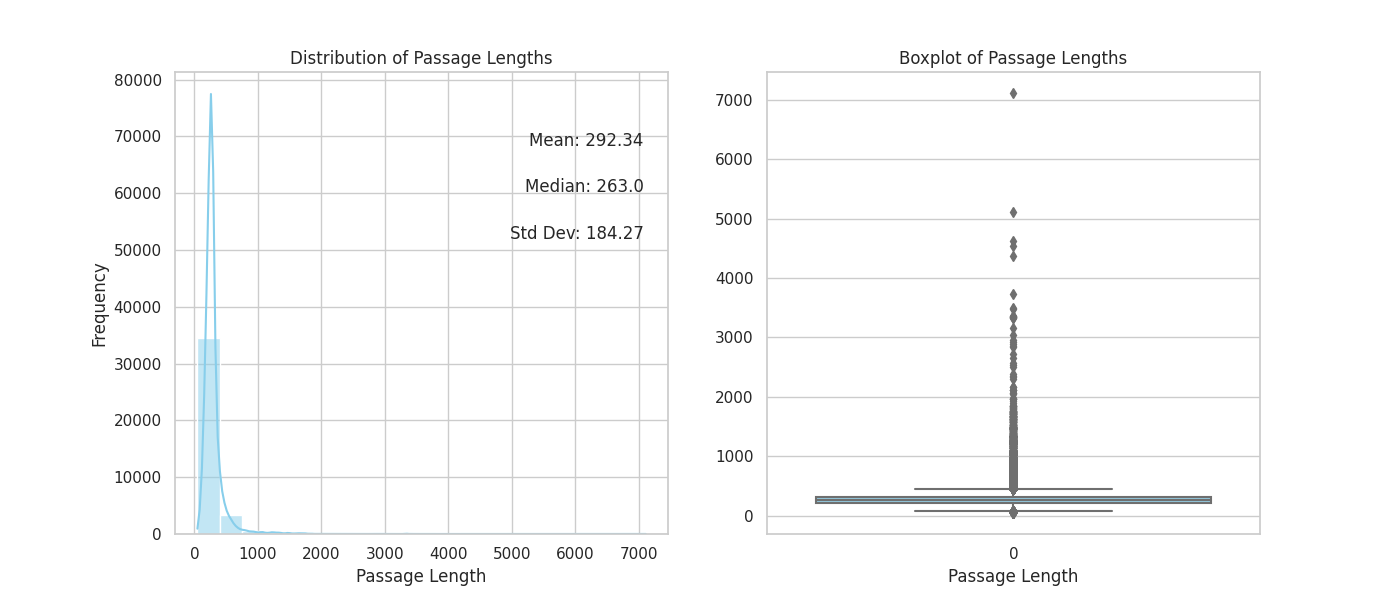
\includegraphics[width=\textwidth]{Grafiken/Statistiken/IndexGerman_Passage_Length_Statistics_old.png}
    \caption{Passage Length Distribution of the German \gls{er} Dataset before Filtering}
    \label{fig:er-german-passage-length-old}
\end{figure}

In Step (3), every passage and all in Step (5) generated questions of the German and English \gls{er} dataset are translated using the Google Translate API. This creates a two more dataset in addition to the existing two, which are directly based on the document's language.

The final Step (4) toward the \textit{knowledge source} is the index creation. To simplify the later \gls{rag} system, the decision was made not to use a hierarchical index structure. However, this could lead to problems when users need to find specific information within one document and want to perform metadata-filtering. To address this, all passages have the title of the document from which they were extracted concatenated to them in the following way:

\begin{quotation}
    \{passage\} + \texttt{ - } + \{documentName\}
\end{quotation}

This approach enables the retriever and reader to identify passages and their corresponding documents in a single step, as opposed to hierarchical index implementations that necessitate multiple steps and potentially multiple databases for embeddings and metadata of the passages. This method has been chosen because, in this use-case, the only utilized and easy extractable metadata of a document is a documents title (e.g., \textit{Examination Regulation for the Master Data and Computer Science}, with some even including the date). Other use-cases may require more complicated appraoches. For the translated datasets, the document name will be translated, as described in Step (3).

\textbf{Data Augmentation:} Step (5) of the extraction pipeline involves data augmentation. For \textit{Question Generation} based on a given passage, the few-shot approach from \textit{PROMPTAGATOR} \cite{dai_promptagator_2022} has been employed. For the English \gls{er} dataset, the following prompt is used to generate a question, given a passage and $i$ examples:

\begin{quote}
   \texttt{System Prompt:}\\
    \texttt{You are an assistant generating one question given a context. Please start your generated question with the indicator 'Generated Question:' Here are some examples:} \\
   \{i\}\texttt{-Example:} \\
   \texttt{Context:} \{passage\} \\
    \texttt{Generated Question:} \{question\} \\ \\
    \texttt{User:} \\
    \texttt{Generate the question based on the following context:}\\
    \{passage\}
    \label{prompt:system-prompt-data-generation}
\end{quote}

The snippet in the System Prompt is looped four times to accommodate the number of examples. The examples represent different question types, which themeself indicate different answer types, in order to add some variety to the generated data. The used examples can be found in the appendix \ref{ref:appendixA-data-augmentation-few-shot-prompt}. The Prompt is generally designed to be used with a chat fine-tuned model, as it showed better results in a qualitative evaluation. For English question generation, the \textit{Llama2-7B-Chat-GPTQ}\footnote{\url{https://huggingface.co/TheBloke/Llama-2-7b-Chat-GPTQ}} is employed. It's a quantized version of the original Llama2-7B-Chat Model by Meta \cite{touvron_llama_2023}. For the German \gls{er}, the same prompt translated to English is used. For the German tasks, the \textit{Leo-Hessianai-7B-Chat-GPTQ}\footnote{\url{https://huggingface.co/TheBloke/leo-hessianai-7B-chat-GPTQ}} model is used, which is a quantized version of a German language fine-tuned Llama2-7B-Chat Model \cite{pluster_leolm_2023}.

It's worth noting that the English Llama2-7B-Chat was capable of directly understanding the system prompt and generating questions with the indicator \texttt{Generated Question}, which made using the generated text easier. However, the German \gls{llm} struggled with this Few-Shot task and often generated multiple responses that didn't start with the indicator \texttt{Generierte Frage}. Additionally, the model sometimes included answers after the questions. To extract the single question from the generated text in the German \gls{llm} output, the text is cropped after a \texttt{:} and \texttt{?}, so the string enclosed by these characters is used as the question for a given passage. 

The choice of Llama2-based models was based on their new state-of-the-art results in multiple benchmarks, as demonstrated by these models in the open-source \gls{llm} niche \cite{touvron_llama_2023}. Additionally, the work of Plüster et al. \cite{pluster_leolm_2023} on LeoLama opens the opportunity to compare the performance of German and English \gls{llm}s from the same family.

For \textit{Answer Generation} the previously generated questions per passage are being used. In order to provide high quality answers, the choice was made to use gpt-3.5-turbo

\subsection{Retriever}
\label{subsec:retriever-impl}

The implemented retrievers can be found in Figure \ref{fig:retriever-implementation}. Given the limited availability of (synthetic) data suitable for fine-tuning, the decision was made to exclusively utilize top-performing \gls{ood} zero-shot retrievers. Fine-tuning a model on such a small dataset could lead to a high risk of overfitting. To assess retriever performance, the synthetic dataset will be used for benchmarking. Among the top-performing retrievers from the BEIR benchmarks, the following three retrievers have been choosen:

\begin{enumerate}
    \item \textbf{BM25:} This employs the standard lexical-based best match algorithm with hyperparameters $k_1=1.5$, $b=0.75$, and $\epsilon=0.25$. It is implemented using the open-source project \textit{rank-bm25} \footnote{\url{https://github.com/dorianbrown/rank_bm25}}.
    \item \textbf{BM25 + CE:} This uses a BM25 retriever in combination with a Cross-Encoder re-ranker, which serves as the baseline established in BEIR \cite{thakur_beir_2021}. This combination continues to perform as the state-of-the-art. The Cross-Encoder utilized is the same as the one in the BEIR baseline implementation: \textit{ms-marco-MiniLM-L-6-v2} \cite{wang_minilm_2020}, specifically the implementation provided on Hugging Face \footnote{\url{https://huggingface.co/cross-encoder/ms-marco-MiniLM-L-6-v2}}. For German indices, a German version of \textit{ms-marco-MiniLM-L-6} is used: \textit{ms-marco-MiniLM-L-6-en-de-v1} \footnote{\url{https://huggingface.co/cross-encoder/msmarco-MiniLM-L6-en-de-v1}}.
    \item \textbf{Large DPR:} For the large \gls{dpr}, the embedding model from OpenAI, \textit{text-embedding-ada-002} \footnote{\url{https://platform.openai.com/docs/models/embeddings}}, is employed. The parameter size of this model is estimated to be around 350 million parameters\cite{muennighoff_sgpt_2022}\footnote{As OpenAI does not publicly provide information on their model specs, there exists only estimates}.
\end{enumerate}

These retrievers have been implemented and evaluated based on the synthetic data, and the results are presented in Section \ref{sec:results}.

\begin{figure}
    \centering
    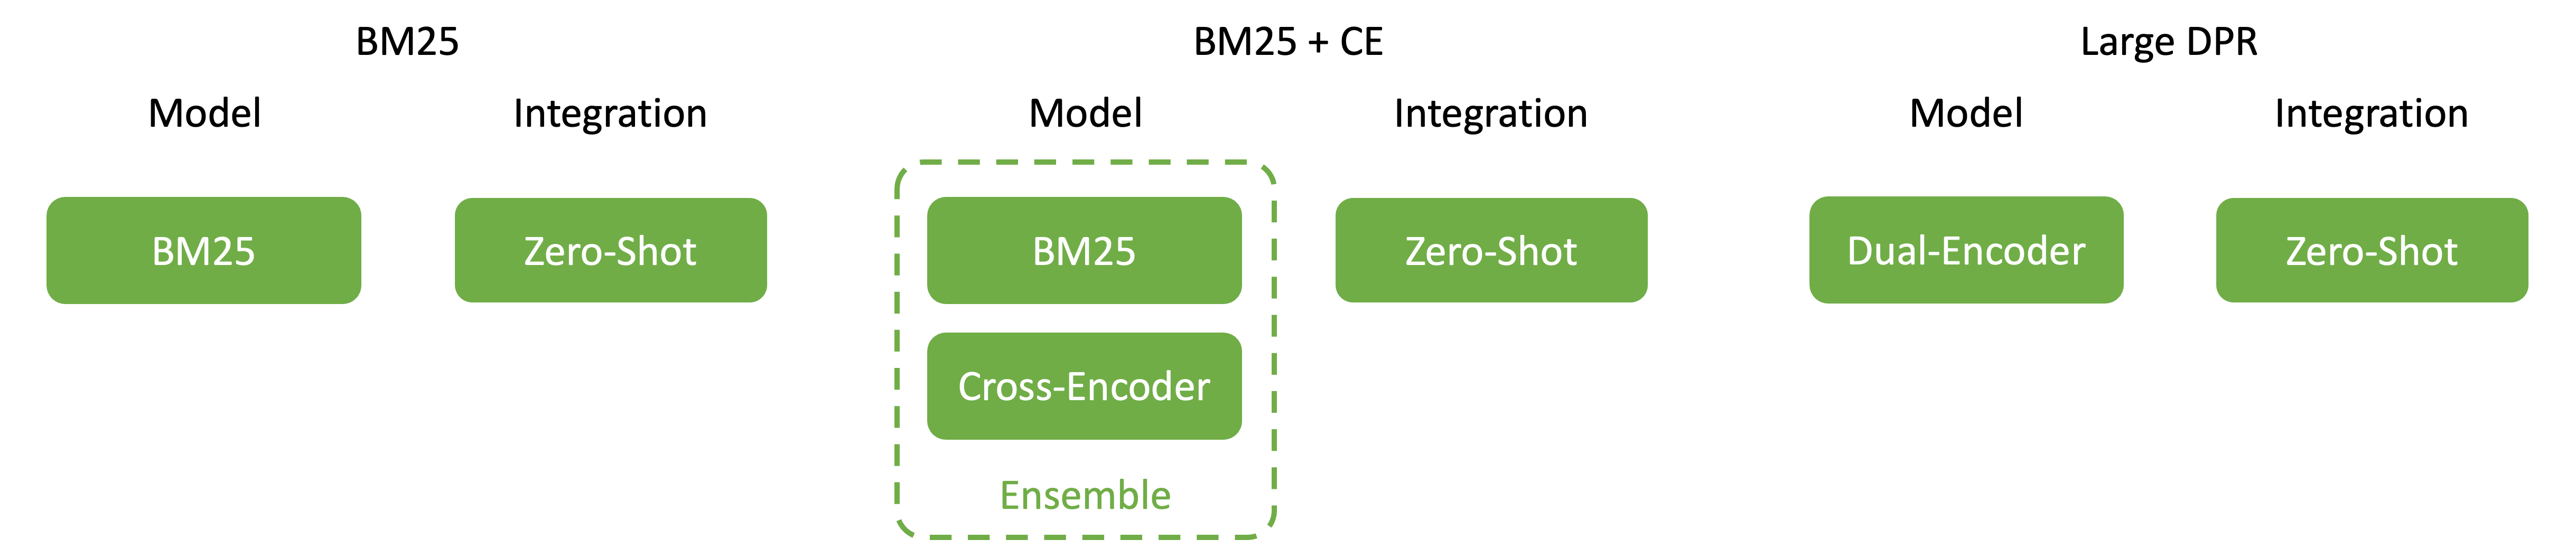
\includegraphics[width=\textwidth]{Grafiken/Evaluation/retriever_implemented.png}    
    \caption{Implemented Retrievers}
    \label{fig:retriever-implementation}
\end{figure}

\subsection{Reader}
\label{subsec:reader-impl}

The implemented readers can be found in Figure \ref{fig:reader-implementation}. Due to the limited hardware resources and high-quality data, the decision was made to only use zero-shot pre-trained \glspl{llm}s for the reader component and not fine-tune any. The following readers have been chosen:

\begin{enumerate}
    \item \textbf{gpt-3.5-turbo:} GPT 3.5 Turbo is part of the OpenAI chat completion family\footnote{\url{https://platform.openai.com/docs/models/gpt-3-5}}. Details on the parameters are not available. However, the latest published research by OpenAI indicates 175B parameters for the model on which GPT 3.5 Turbo was built. In general, the model is an \gls{llm} trained using human feedback on chat-like completion tasks \cite{ouyang_training_2022}. It accepts up to 4,096 tokens as input.
    \item \textbf{Llama2-7B-Chat-GPTQ:} This is a quantized version of the original Llama2-7B-Chat Model by Meta \cite{touvron_llama_2023}. The model is an \gls{llm} trained on chat-instruction datasets \cite{ouyang_training_2022}. The model is available on Hugging Face\footnote{\url{https://huggingface.co/TheBloke/Llama-2-7b-Chat-GPTQ}}. The model is quantized using GPTQ \cite{muennighoff_sgpt_2022}. However, the provider did not report any benchmarks indicating the accuracy drop of the GPTQ version compared to the original. It accepts up to 4,096 tokens as input.
    \item \textbf{leo-hessianai-7B-chat-GPTQ:} \textit{Linguistisch Erweitertes Offenes Language Model} (LeoLM) is a German tasks fine-tuned version of the original Llama2-7B-Chat model. The original Llama2 is fine-tuned on a large corpus of German language texts, and multiple adjustments are applied to overcome the problem of forgetting. This results in a maximum input token length of 8,000 tokens. In addition to original German chat instruction-based datasets, automatic translated English benchmark datasets are used as well. Benchmarking results indicate an increase in German language capabilities while maintaining English language task performance \cite{pluster_leolm_nodate}.
\end{enumerate}

Generally, \textbf{gpt-3.5-turbo} acts as a higher-end benchmark. It is a state-of-the-art \gls{llm} with high popularity in the media and developer community. \textbf{Llama2-7B-Chat-GPTQ} should be a hardware resource-efficient alternative pre-trained model, especially the quantized version that can run on consumer hardware. \textbf{leo-hessianai-7B-chat-GPTQ} is representative of a German native model, providing further insights into language dependencies and the performance of \gls{llm}s, as the use case involves multiple indices in German and English.

Further approaches such as evaluating different fine-tuning approaches have been excluded, as they would open a huge problem field itself and can't be covered in an appropriate manner in this thesis. Therefore this thesis rather focuses on a holistic \gls{poc} to show and evaluate one possible implementation approach of the in Section \ref{chap:main} introduced framework using the mentioned \gls{llm}s.

\begin{figure}
    \centering
    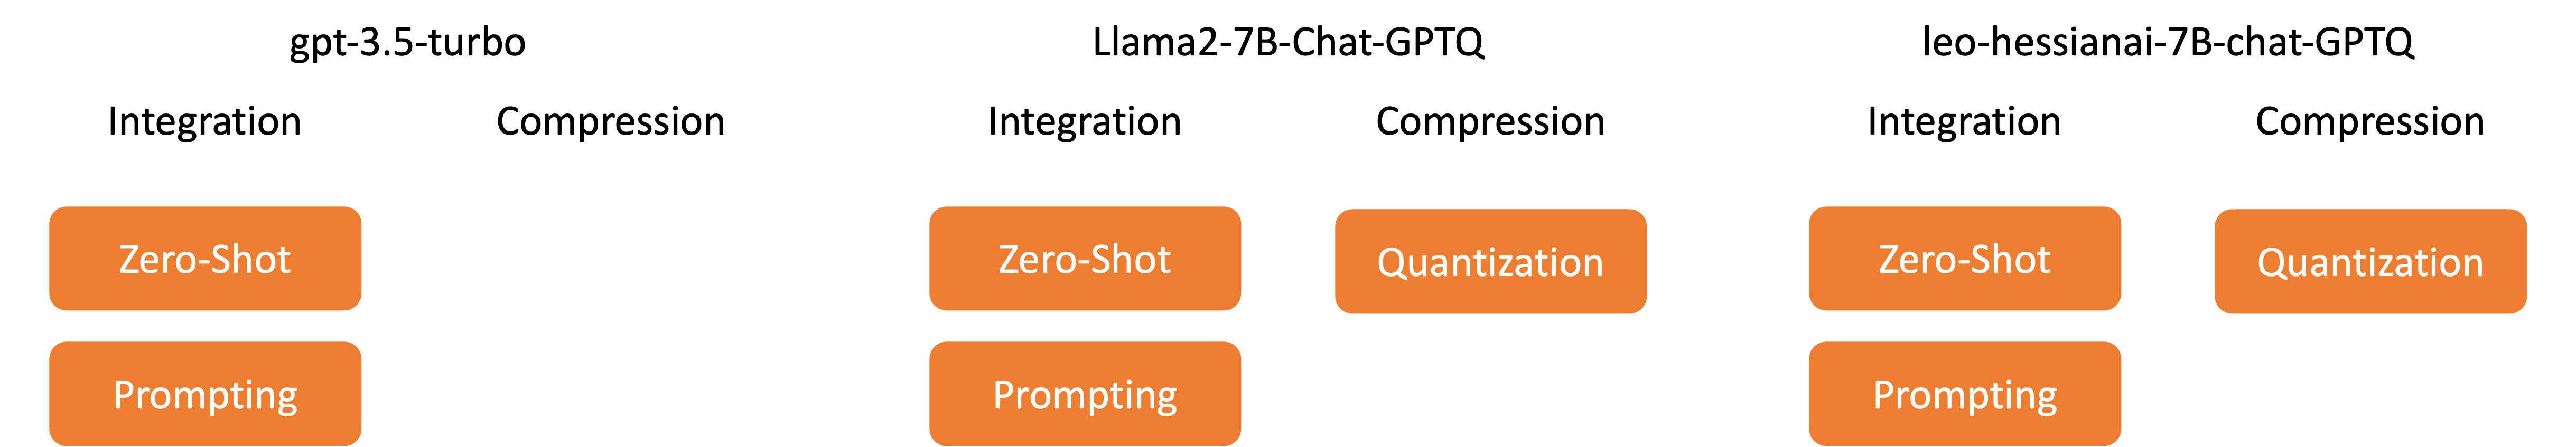
\includegraphics[width=\textwidth]{Grafiken/Evaluation/reader_implemented.png}
    \caption{Implemented Readers}
    \label{fig:reader-implementation}
\end{figure}

\subsection{CQU}
\label{subsec:cqu-impl}

\section{Experimental Results}
\label{sec:results}

This section evaluates the implemented system and the introduced framework, using metrics introduced in Section \ref{sec:metrics}. The evaluation covers the following components: \textit{Extraction}, especially synthetic data generation (Section \ref{subsec:data-augmentation-quality}), \textit{Retriever} (Section \ref{subsec:retrieval-results}), \textit{Reader} (Section \ref{subsec:reader-results}), and the complete \gls{convqa} system (Section \ref{subsec:convqa-results}). The evaluation is based on the synthetic dataset described in Section \ref{subsec:index}, generated from the dataset introduced in Section \ref{sec:data}.

\subsection{Data Augmentation Quality}
\label{subsec:data-augmentation-quality}

\begin{figure}
    \centering
    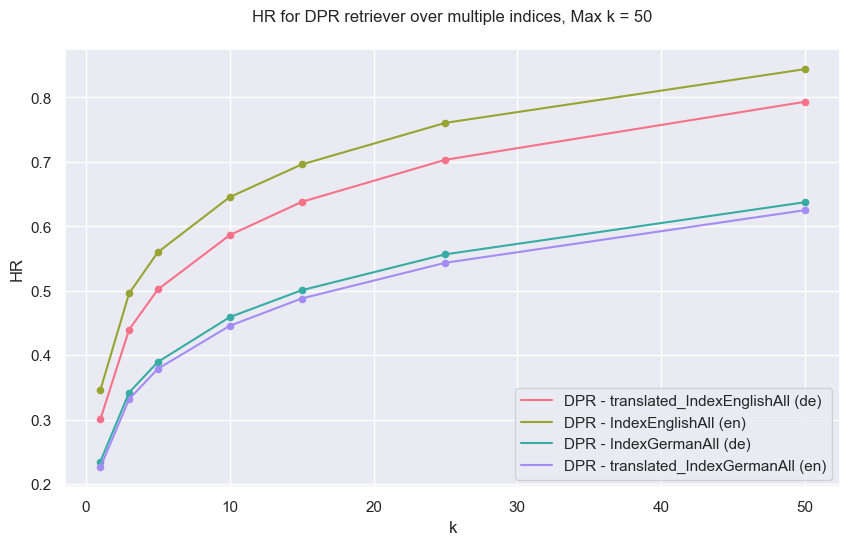
\includegraphics[width=\textwidth]{Grafiken/Evaluation/Data_Generation/hr_dpr_all_400.png}
    \caption{Retriever performance comparison over all datasets}
    \label{fig:synthetic-data-generation-performance-comparison}
\end{figure}

As detailed in Section \ref{subsec:index}, the two main indices, namely \textit{indexEnglish} and \textit{indexGerman}, are based on the corresponding \gls{er}s. During the generation of the question-context datasets, qualitative issues arose when using \textit{leo-hessianai-7B-chat-GPTQ}. As indicated by System Prompt \ref{prompt:system-prompt-data-generation}, the model was prompted to start the generated answer after a defined indication text. In multiple cases, the German model \textit{leo-hessianai-7B-chat-GPTQ} was unable to fulfill this request, necessitating post-processing as described in Section \ref{subsec:index}. This issue was not present when using the English model \textit{Llama2-7B-Chat-GPTQ}. 

In addition to this qualitative issue, a quantitative evaluation is possible when comparing the retrieval performance on both datasets and their translated versions: \textit{translated-indexEnglish} and \textit{translated-indexGerman}. The performance results of the large \gls{dpr} retriever are shown in Figure \ref{fig:synthetic-data-generation-performance-comparison}. They indicate, despite a small language performance gap, a significant difference in performance between the two indices \textit{indexEnglish} and \textit{indexGerman} and their corresponding translated versions. This suggests poorer question generation quality for \textit{indexGerman}, as observed in the following example:

\begin{quote}
% \begin{lstlisting}[breaklines, escapeinside={(*@}{@*)}]
\begin{verbatim}
Generierte Antwort:
Was ist der Wert von $(4+5) \\times {(4+5) \\div {2 \\div {1 \\
times {2}}}}$, wobei die mündliche Prüfung von einer Person 
abgenommen wird, die nicht prüft?

Gegebener Kontext:
Das Ergebnis ist der zu prüfenden Person im Anschluss an die münd-
liche Prüfung bekannt zu geben.\n\n(4) (5) Mündliche Prüfungen 
werden vor einer prüfenden Person in Gegenwart einer beisitzen-
den Person gem. 6 Abs.\n\n4 abgelegt. - Prüfungsordnung Mathematik 
MA (2022-10-05)
\end{verbatim}
% \end{lstlisting}
\end{quote}


\subsection{Retrieval Results}
\label{subsec:retrieval-results}

\subsection{Reader Results}
\label{subsec:reader-results}

\subsection{Conversational Question Answering Results}
\label{subsec:convqa-results}

%%%%%%%%%%%%%%%%%%%%%%%%%%%%%%%%%%%%%%%%%%%%%%%%%%%%%%%%%%%%%
\newpage
%%%%%%%%%%%%%%%%%%%%%%%%%%%%%%%%%%%%%%%%%%%%%%%%%%%%%%%%%%%%

\chapter{Conclusions and Future Work}
\label{chap:concl}

This thesis serves as an introduction guide for developing conversational question-answering systems tailored to specific use cases. Beginning with an extensive overview of the field in Section \ref{chap:grundlagen}, we delve into the essential algorithms and concepts necessary for constructing such systems.

Focusing on practical implementations, Section \ref{chap:main} narrows down the implementation landscape by focusing on conversational retrieval-augmented generators for question-answering. We outline a system comprising four distinct components: Extract, CQU, Retriever, and Reader. Each component addresses its own well-defined problem domain, shedding light on the major challenges associated with them. Notable contributions include the detailed breakdown of the often-overlooked Extract component into various operations and the identification of challenges faced by the Retriever component, both with the knowledge base and the evidence set for the Reader. Additionally, we dissect the tasks of the Reader component into smaller challenges and propose multiple existing and novel solutions to tackle them. Ultimately, the main contribution lies in providing a decision map for constructing a conversational question-answering system, based on the diverse components and implementation possibilities.

To validate the feasibility of the decision map, Section \ref{chap:eval} presents the construction and evaluation of a default system primarily based on zero-shot components. Various evaluation approaches are introduced, implemented, and tested within this framework. Notably, the component-wise evaluation using synthetic data yields insights into the feasibility of synthetic datasets for metric-based component evaluation. Challenges such as complex or abstract questions pose difficulties in using synthetic datasets containing tuples of question-answer pairs and evidence, particularly applicable for factoid questions. Furthermore, the performance of two smaller \gls{llm}s, \textit{leo-hessian-7B-chat} and \textit{Llama2-7B-chat}, is compared against \textit{gpt-3.5-turbo}. Performance issues in applications of the smaller \gls{llm}s are identified, necessitating considerations when utilizing them in conversational question-answering systems. These issues primarily revolve around consistency in text generation quality and the suitability of the \gls{llm}s for the role of a Reader in the conversational setting, attributed to their inferior capabilities compared to larger \gls{llm}s in identifying pertinent information from the evidence set.

In Section \ref{subsec:data-augmentation-quality}, we discuss the identified limitations of the chosen approaches, which is necessary reading for anyone interested in building their own conversational question-answering system and how to evaluate it.

\vspace{\baselineskip}
\noindent We recommend any reader interested in building their own conversational question-answering system to start with this thesis as a foundational guide. They can then proceed to build a basic system similar to Section \ref{sec:setup} and evaluate it in an end-to-end manner as described in Section \ref{subsec:rag-eval}. This approach provides the quickest way to understand the specific challenges of their use case and how to further iterate and improve their system.

\vspace{\baselineskip}
\noindent Regarding future work, we propose the following directions for research:
\begin{itemize}
    \item \textbf{Practical Feasibility of Conversational Question Answering Systems:} Evaluate the costs and user experience associated with implementing conversational question-answering systems, particularly considering the significant expenses linked with utilizing \gls{llm}s. This evaluation should delve into whether it is financially viable to construct a search system relying on \gls{llm}s, especially given the escalating costs associated with the growing complexity of utilized approaches and the increasing number of \gls{llm} inference runs required. 

    \item \textbf{Constrained System Design:} Develop a search system that strikes a balance between resource utilization and search result quality. This endeavor may entail amalgamating multiple system components, implementing post-processing techniques on the evidence set, and orchestrating a series of reader components to create a system capable of addressing diverse question types while maintaining efficient resource usage. Relying solely on \gls{llm}-based approaches, such as \gls{rag}, may not always be the optimal solution for all use cases and setups. It might be more resource-efficient to employ a combination of smaller \gls{llm}s for different subtasks, or to explore techniques like quantization and incorporating extractive readers as post-processing steps, among others.

    \item \textbf{Improving the Retriever Component:} Enhance the performance of the retriever component, specifically focusing on its ability to locate all relevant contexts within the evidence set. This endeavor could entail investigating novel methodologies, such as employing agent-like retrievers or capitalizing on the structural elements of documents to direct the extraction and retrieval process. E.g. aligning the retrieval process with the search strategies employed by humans, who often hierarchically navigate through documents to pinpoint relevant passages, may offer valuable insights for enhancing retriever performance.

    \item \textbf{PDF Data Extraction:} Develop a universal solution for extracting textual or multimodal information from PDFs. This includes addressing the challenges of existing extraction operations, which yield different document models and may produce inconsistent passages. 
\end{itemize}

% References (Literaturverzeichnis):
% a) Style (with abbreviations: use alpha):
% see
% https://de.wikibooks.org/wiki/LaTeX-W%C3%B6rterbuch:_bibliographystyle
% for the different formats and styles

% \bibliographystyle{apalike}
\bibliographystyle{unsrt}
% b) The File:
\bibliography{references}

\end{document}